% =====================================================================
%  CHAPITRE 5 — PRÉSENTATION DES RÉSULTATS
%  Mémoire : Analyse et Modélisation du Risque d'Insécurité Alimentaire
%            des Ménages au Bénin (données AGVSAN 2017)
%  Auteur  : DAHOUI Pinel Baudelaire T. — Master SAV, CIPMA / Chaire UNESCO
%
%  Packages requis dans le préambule du document maître :
%    \usepackage{graphicx}   % figures
%    \usepackage{booktabs}   % filets de tableaux (\toprule, \midrule, \bottomrule)
%    \usepackage{float}      % placement [H]
%    \usepackage{amsmath}    % mathématiques
%  Les figures sont lues depuis le dossier outputs/ du pipeline Python :
%    \graphicspath{{outputs/}{./outputs/}}
%  Ce fichier s'insère par : % =====================================================================
%  CHAPITRE 5 — PRÉSENTATION DES RÉSULTATS
%  Mémoire : Analyse et Modélisation du Risque d'Insécurité Alimentaire
%            des Ménages au Bénin (données AGVSAN 2017)
%  Auteur  : DAHOUI Pinel Baudelaire T. — Master SAV, CIPMA / Chaire UNESCO
%
%  Packages requis dans le préambule du document maître :
%    \usepackage{graphicx}   % figures
%    \usepackage{booktabs}   % filets de tableaux (\toprule, \midrule, \bottomrule)
%    \usepackage{float}      % placement [H]
%    \usepackage{amsmath}    % mathématiques
%  Les figures sont lues depuis le dossier outputs/ du pipeline Python :
%    \graphicspath{{outputs/}{./outputs/}}
%  Ce fichier s'insère par : % =====================================================================
%  CHAPITRE 5 — PRÉSENTATION DES RÉSULTATS
%  Mémoire : Analyse et Modélisation du Risque d'Insécurité Alimentaire
%            des Ménages au Bénin (données AGVSAN 2017)
%  Auteur  : DAHOUI Pinel Baudelaire T. — Master SAV, CIPMA / Chaire UNESCO
%
%  Packages requis dans le préambule du document maître :
%    \usepackage{graphicx}   % figures
%    \usepackage{booktabs}   % filets de tableaux (\toprule, \midrule, \bottomrule)
%    \usepackage{float}      % placement [H]
%    \usepackage{amsmath}    % mathématiques
%  Les figures sont lues depuis le dossier outputs/ du pipeline Python :
%    \graphicspath{{outputs/}{./outputs/}}
%  Ce fichier s'insère par : % =====================================================================
%  CHAPITRE 5 — PRÉSENTATION DES RÉSULTATS
%  Mémoire : Analyse et Modélisation du Risque d'Insécurité Alimentaire
%            des Ménages au Bénin (données AGVSAN 2017)
%  Auteur  : DAHOUI Pinel Baudelaire T. — Master SAV, CIPMA / Chaire UNESCO
%
%  Packages requis dans le préambule du document maître :
%    \usepackage{graphicx}   % figures
%    \usepackage{booktabs}   % filets de tableaux (\toprule, \midrule, \bottomrule)
%    \usepackage{float}      % placement [H]
%    \usepackage{amsmath}    % mathématiques
%  Les figures sont lues depuis le dossier outputs/ du pipeline Python :
%    \graphicspath{{outputs/}{./outputs/}}
%  Ce fichier s'insère par : \input{Chapitre_5_Resultats}
% =====================================================================

\section{Présentation des résultats}
\label{sec:resultats}

Ce chapitre présente les résultats produits par le pipeline analytique décrit au
chapitre~4, exécuté sous \texttt{Python}~3.11 (\emph{notebook}
\texttt{Pipeline\_Insecurite\_Alimentaire\_Benin.ipynb}, graine aléatoire
\texttt{RANDOM\_STATE = 42}). La présentation suit la progression logique des
objectifs spécifiques : constitution et validation de la variable dépendante
(Section~\ref{ssec:res-echantillon}), analyse descriptive univariée et bivariée
(Sections~\ref{ssec:res-univarie} à~\ref{ssec:res-bivarie}), identification des
déterminants — OS1 (Section~\ref{ssec:res-os1}), comparaison des modèles
prédictifs — OS2 (Section~\ref{ssec:res-os2}), interprétabilité \textsc{shap}
(Section~\ref{ssec:res-shap}), cartographie communale du risque — OS3
(Section~\ref{ssec:res-os3}) et produits opérationnels pour l'outil d'aide à la
décision — OS4 (Section~\ref{ssec:res-os4}). Une synthèse confronte enfin les
résultats aux hypothèses de recherche (Section~\ref{ssec:res-hypotheses}).

% ---------------------------------------------------------------------
\subsection{Constitution de l'échantillon analytique et validation de la variable dépendante}
\label{ssec:res-echantillon}

\subsubsection{Échantillon analytique et prévalence de l'insécurité alimentaire}

La base AGVSAN 2017 compte 14\,952 ménages et 1\,406 variables. La variable
\texttt{Round\_INDICE\_SECAL} est renseignée pour la totalité des ménages :
aucune observation n'a été exclue et l'échantillon analytique est de
$n = 14\,952$. La Table~\ref{tab:res-repartition-y} présente la répartition des
quatre classes \textsc{cari} et les prévalences associées aux trois définitions
de la variable dépendante.

\begin{table}[H]
\centering
\caption{Répartition des classes \textsc{cari} et prévalence de $Y$ selon les trois définitions}
\label{tab:res-repartition-y}
\small\setlength{\tabcolsep}{4pt}
\begin{tabular}{lrr}
\toprule
\textbf{Classe \textsc{cari}} & \textbf{Effectif} & \textbf{\%} \\
\midrule
1 — Sécurité alimentaire          & 6\,998 & 46,80 \\
2 — Sécurité alimentaire limite   & 6\,452 & 43,15 \\
3 — Insécurité modérée            & 1\,378 &  9,22 \\
4 — Insécurité sévère             &    124 &  0,83 \\
\midrule
\textbf{Définition de $Y$}        & \textbf{Prévalence brute} & \textbf{Prévalence pondérée} \\
\midrule
Référence $\{3,4\}$               & 10,05\,\% & 9,66\,\% \\
Stricte $\{4\}$                   &  0,83\,\% & --- \\
Élargie $\{2,3,4\}$               & 53,20\,\% & --- \\
\bottomrule
\end{tabular}
\end{table}

Selon la définition de référence, 1\,502 ménages (10,05\,\% ; 9,66\,\% après
pondération par les poids d'enquête \texttt{weight\_agvsa}) sont en insécurité
alimentaire. Ce fort déséquilibre de classes justifie \emph{a posteriori} la
stratégie de \emph{class weighting} retenue au chapitre~4 (Section~4.5.2). La
prévalence pondérée est nettement différenciée selon le milieu de résidence :
13,03\,\% en milieu rural contre 6,19\,\% en milieu urbain (et 1,52\,\%
seulement à Cotonou), premier indice de la dimension territoriale du phénomène.

\subsubsection{Validation croisée de la classification officielle}

Conformément à la Section~4.2.4, le \textsc{sca} a été reconstruit de manière
indépendante à partir des 18~items bruts de consommation alimentaire
(moyenne~=~49,8 ; médiane~=~50,5 ; étendue 0--112). Sa répartition selon les
seuils standard du \textsc{pam} est : pauvre ($<28$) 1\,435 ménages (9,6\,\%),
limite (28--42) 3\,387 (22,7\,\%), acceptable ($>42$) 10\,130 (67,7\,\%). La
concordance entre le \textsc{sca} reconstruit dichotomisé
($\textsc{sca} \leq 42$) et la classification officielle dichotomisée s'établit
à \textbf{76,1\,\% d'accord global} avec un \textbf{Kappa de Cohen de 0,333},
et la corrélation ordinale entre le \textsc{sca} et la classe \textsc{cari} est
négative et hautement significative (Spearman $\rho = -0{,}371$ ;
$p < 0{,}001$), dans le sens attendu (un \textsc{sca} plus faible correspond à
une classe plus sévère). Cette concordance modérée est conforme à la
littérature : la classification \textsc{cari} officielle combine le \textsc{sca}
avec le \textsc{rcsi} et la part des dépenses alimentaires, de sorte qu'une
concordance parfaite avec le seul \textsc{sca} n'est pas attendue.

La validation par l'indice de stratégies de survie confirme la cohérence de la
variable dépendante : le \textsc{rcsi} moyen est de 18,96 chez les ménages en
insécurité contre 10,79 chez les ménages en sécurité (test unilatéral de
Mann-Whitney, $p = 2{,}2 \times 10^{-66}$).

\paragraph{Limite relative au \textsc{hfias}.} Le score \textsc{hfias} prévu
comme second indicateur de validation (Section~4.2.5) s'est révélé
\textbf{indisponible} dans la base ménage transmise (la colonne \texttt{Q\_9\_05}
du fichier correspond à un autre champ du questionnaire). La validation croisée
repose donc sur le seul \textsc{rcsi}, limite qui sera discutée au chapitre
suivant.

% ---------------------------------------------------------------------
\subsection{Analyse univariée des variables focales}
\label{ssec:res-univarie}

\subsubsection{Situation alimentaire des ménages}

Au niveau national, 89,95\,\% des ménages sont en sécurité alimentaire et
10,05\,\% en insécurité (90,34\,\% et 9,66\,\% après pondération ;
Figure~\ref{fig:res-y-national}). La stratification par département
(Figure~\ref{fig:res-y-departement}) révèle de fortes disparités : la
prévalence brute varie de 1,52\,\% dans le Littoral à \textbf{22,80\,\% dans
l'Atacora}, suivi du Couffo (16,40\,\%), des Collines (15,74\,\%) et du Zou
(11,63\,\%), tous au-dessus de la moyenne nationale. Cette hétérogénéité
géographique, déjà visible au stade descriptif, annonce les résultats de la
cartographie prédictive (Section~\ref{ssec:res-os3}).

\begin{figure}[H]
\centering
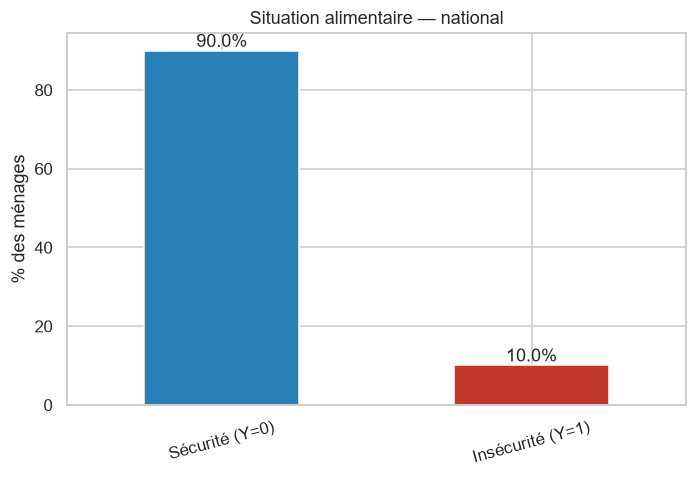
\includegraphics[width=0.62\textwidth]{outputs/univarie_Y_national.png}
\caption{Répartition nationale des ménages selon la situation alimentaire ($Y$)}
\label{fig:res-y-national}
\end{figure}

\begin{figure}[H]
\centering
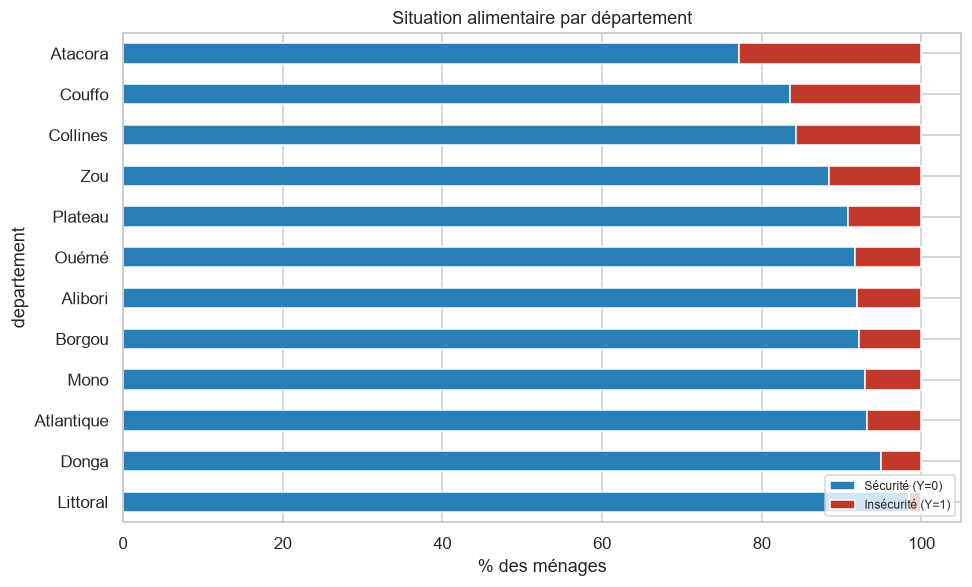
\includegraphics[width=0.85\textwidth]{outputs/univarie_Y_departement.png}
\caption{Situation alimentaire des ménages par département (barres empilées, \% en ligne)}
\label{fig:res-y-departement}
\end{figure}

\subsubsection{Taille des ménages}

La taille moyenne des ménages est de 6,83 personnes (médiane~=~6 ;
écart-type~=~4,57 ; CV~=~66,9\,\%), avec une distribution asymétrique à droite
(skewness~=~2,88) s'étirant jusqu'à 86 personnes
(Figure~\ref{fig:res-taille-hist}). Les ménages ruraux sont en moyenne plus
grands que les ménages urbains (7,2 contre 6,4 personnes ;
Figure~\ref{fig:res-taille-box}), les percentiles extrêmes confirmant cet écart
($P_{90}$ de 13 en milieu rural contre 11 en milieu urbain).

\begin{figure}[H]
\centering
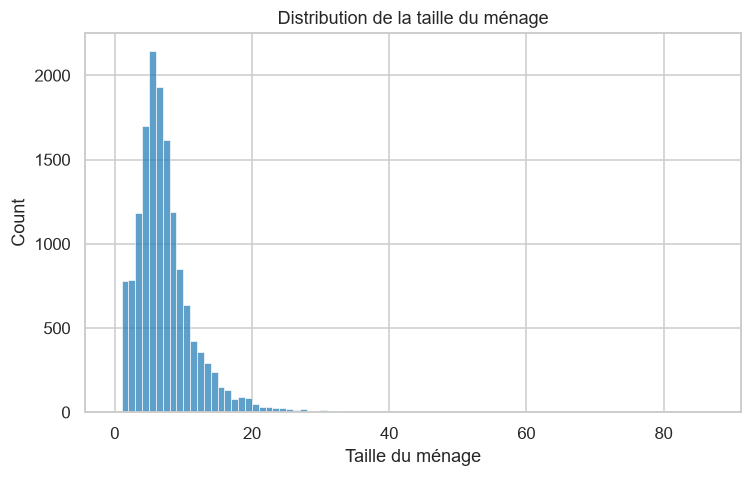
\includegraphics[width=0.62\textwidth]{outputs/univarie_taille_hist.png}
\caption{Distribution de la taille des ménages}
\label{fig:res-taille-hist}
\end{figure}

\begin{figure}[H]
\centering
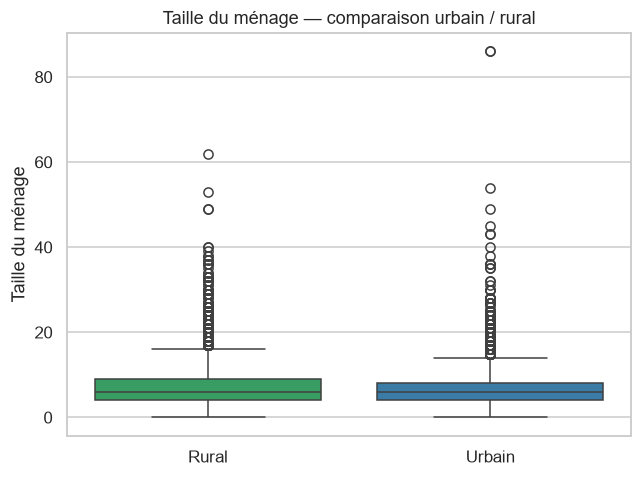
\includegraphics[width=0.55\textwidth]{outputs/univarie_taille_boxplot.png}
\caption{Taille des ménages : comparaison urbain / rural (boîtes à moustaches)}
\label{fig:res-taille-box}
\end{figure}

\subsubsection{Revenu mensuel}

Le revenu mensuel déclaré présente l'asymétrie extrême caractéristique des
données de revenu : moyenne de 68\,105 \textsc{fcfa} pour une médiane de
15\,000 \textsc{fcfa}, écart-type de 217\,941 \textsc{fcfa}
(CV~=~320\,\%), skewness de 11,06 et kurtosis de 181,8
(Figure~\ref{fig:res-revenu-brut}). La transformation logarithmique
$\ln(\text{revenu}+1)$ retenue pour la modélisation (Section~4.3.3) ramène la
skewness à $-0{,}06$, soit une distribution quasi symétrique
(Figure~\ref{fig:res-revenu-log}), ce qui valide empiriquement ce choix
méthodologique.

\begin{figure}[H]
\centering
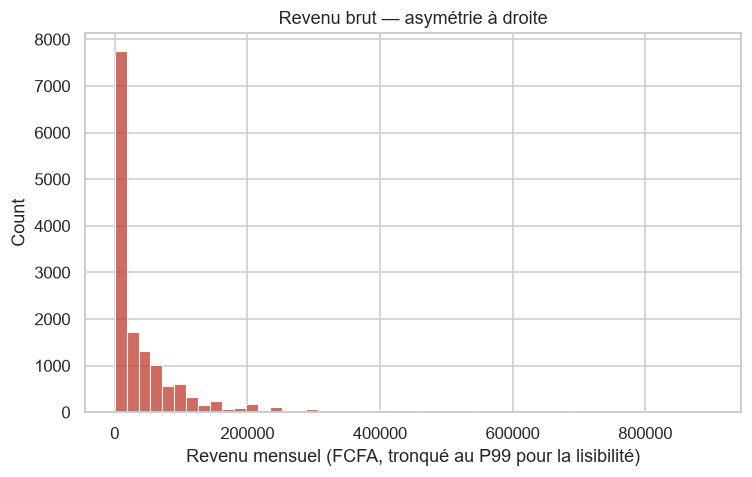
\includegraphics[width=0.62\textwidth]{outputs/univarie_revenu_brut.png}
\caption{Distribution du revenu mensuel brut (\textsc{fcfa}, tronqué au $P_{99}$)}
\label{fig:res-revenu-brut}
\end{figure}

\begin{figure}[H]
\centering
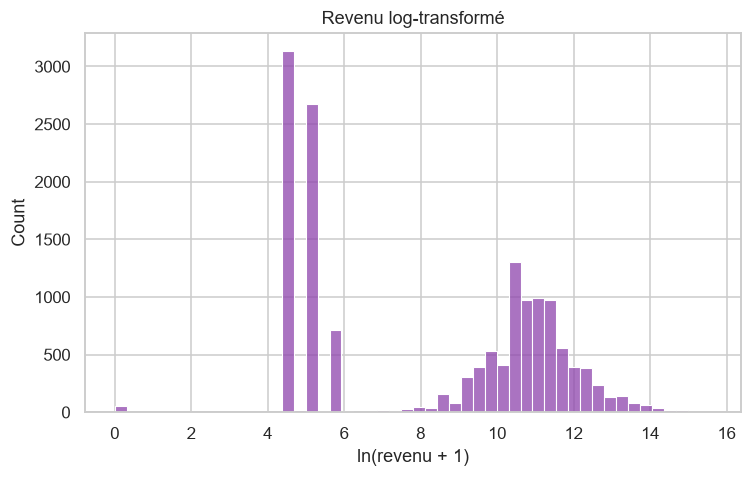
\includegraphics[width=0.62\textwidth]{outputs/univarie_revenu_log.png}
\caption{Distribution du revenu log-transformé $\ln(\text{revenu}+1)$}
\label{fig:res-revenu-log}
\end{figure}

\subsubsection{Âge du chef de ménage}

L'âge moyen du chef de ménage est de 47,1 ans (médiane~=~45 ;
écart-type~=~15,0 ; étendue 16--100 ans), avec une asymétrie modérée
(skewness~=~0,70 ; Figure~\ref{fig:res-age}). La répartition par tranches
usuelles est la suivante : moins de 30~ans, 8,94\,\% ; 30--44~ans, 37,22\,\% ;
45--59~ans, 32,30\,\% ; 60~ans et plus, 21,54\,\%.

\begin{figure}[H]
\centering
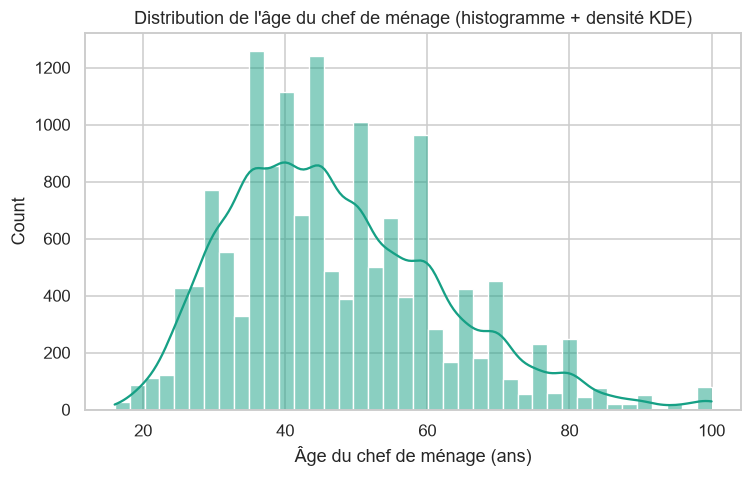
\includegraphics[width=0.62\textwidth]{outputs/univarie_age.png}
\caption{Distribution de l'âge du chef de ménage (histogramme et densité à noyau)}
\label{fig:res-age}
\end{figure}

\subsubsection{Niveau d'instruction du chef de ménage}

Plus de la moitié des chefs de ménage (51,22\,\%) n'ont aucune instruction
formelle ; viennent ensuite le primaire (22,59\,\%), le secondaire (17,04\,\%),
le supérieur (4,47\,\%), l'alphabétisation (3,36\,\%), l'école coranique
(1,17\,\%) et le cursus arabe (0,06\,\%) (Figure~\ref{fig:res-instruction}).
Après recodage en trois niveaux (Table~5 du chapitre~4), la répartition est :
\emph{Aucun/informel} 55,89\,\%, \emph{Primaire} 22,59\,\%,
\emph{Secondaire et plus} 21,52\,\%.

\begin{figure}[H]
\centering
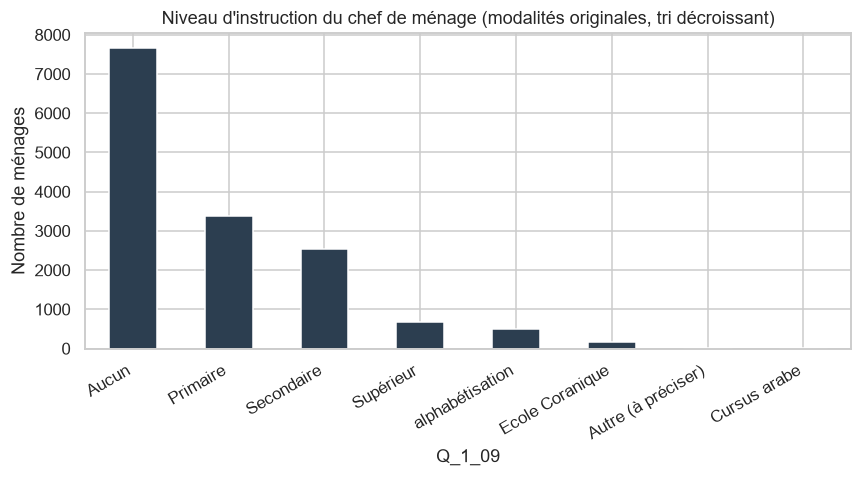
\includegraphics[width=0.72\textwidth]{outputs/univarie_instruction.png}
\caption{Niveau d'instruction du chef de ménage (modalités originales, tri décroissant)}
\label{fig:res-instruction}
\end{figure}

\subsubsection{Accès au crédit}

Un peu plus du quart des ménages (25,79\,\% ; 26,26\,\% pondéré) a contracté un
emprunt au cours des douze derniers mois. L'accès au crédit est légèrement plus
fréquent en milieu rural (27,31\,\%) qu'en milieu urbain (23,99\,\%)
(Figure~\ref{fig:res-credit-univ}).

\begin{figure}[H]
\centering
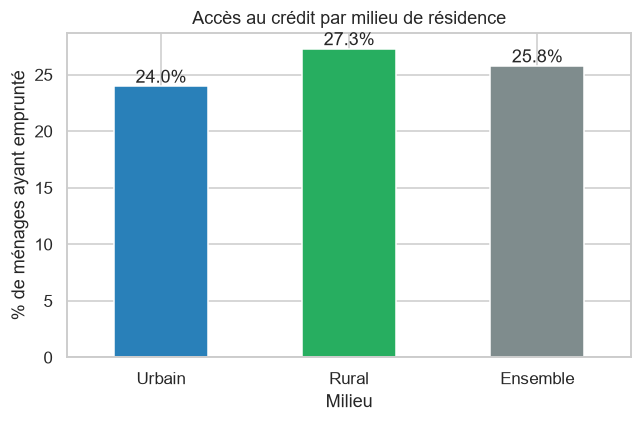
\includegraphics[width=0.55\textwidth]{outputs/univarie_credit.png}
\caption{Proportion de ménages ayant accès au crédit, par milieu de résidence}
\label{fig:res-credit-univ}
\end{figure}

% ---------------------------------------------------------------------
\subsection{Tests de normalité des variables continues}
\label{ssec:res-normalite}

La Table~\ref{tab:res-normalite} rapporte les tests de normalité prévus à la
Section~4.4.3. Pour les quatre variables continues focales, l'hypothèse de
normalité est rejetée par le test de Kolmogorov-Smirnov comme par celui de
Shapiro-Wilk ($p < 0{,}001$ dans tous les cas), conclusion corroborée par les
coefficients de forme et par les QQ-plots
(Figures~\ref{fig:res-qq-taille} et~\ref{fig:res-qq-age}). Conformément à la
règle de décision du chapitre~4 — et en tenant compte de la puissance très
élevée de ces tests avec $n \approx 15\,000$ — l'analyse bivariée recourt
systématiquement au test non paramétrique de Mann-Whitney pour les variables
continues.

\begin{table}[H]
\centering
\caption{Tests de normalité des variables continues focales ($n = 14\,952$)}
\label{tab:res-normalite}
\small\setlength{\tabcolsep}{4pt}
\begin{tabular}{lrrrrrl}
\toprule
\textbf{Variable} & \textbf{KS $D_n$} & \textbf{KS $p$} & \textbf{Shapiro $W$} & \textbf{Skew.} & \textbf{Kurt.} & \textbf{Conclusion} \\
\midrule
Taille du ménage        & 0,164 & $<0{,}001$ & 0,813 &  2,88 & 22,24  & Normalité rejetée \\
Revenu brut (\textsc{fcfa}) & 0,377 & $<0{,}001$ & 0,267 & 11,06 & 181,85 & Normalité rejetée \\
$\ln(\text{revenu}+1)$  & 0,239 & $<0{,}001$ & 0,848 & $-0{,}06$ & $-1{,}54$ & Normalité rejetée \\
Âge du chef de ménage   & 0,092 & $<0{,}001$ & 0,969 &  0,70 & 0,33   & Normalité rejetée \\
\bottomrule
\end{tabular}
\end{table}

\begin{figure}[H]
\centering
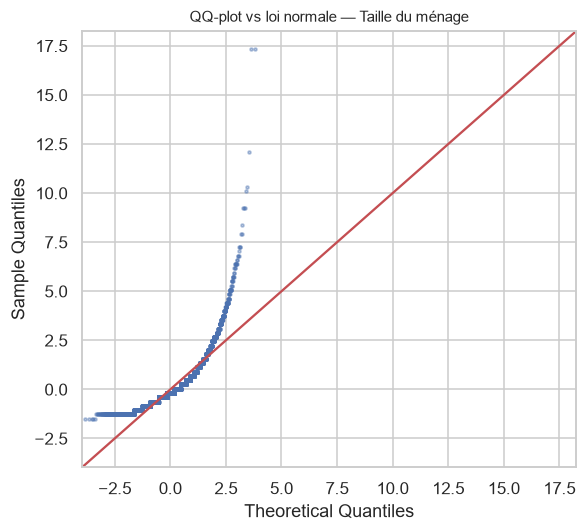
\includegraphics[width=0.48\textwidth]{outputs/normalite_qq_taille.png}
\caption{QQ-plot de la taille du ménage contre la loi normale standard}
\label{fig:res-qq-taille}
\end{figure}

\begin{figure}[H]
\centering
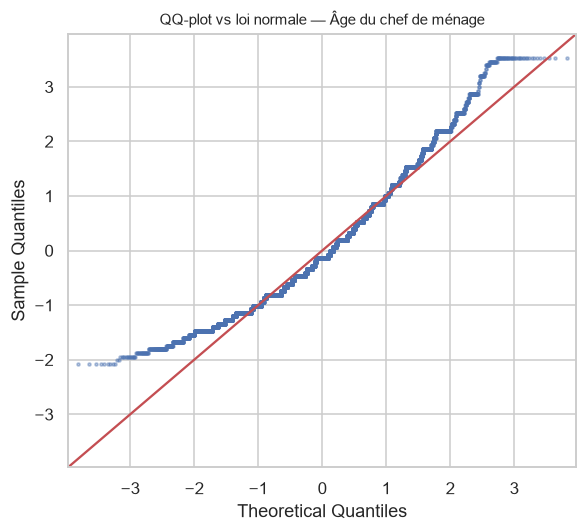
\includegraphics[width=0.48\textwidth]{outputs/normalite_qq_age.png}
\caption{QQ-plot de l'âge du chef de ménage contre la loi normale standard}
\label{fig:res-qq-age}
\end{figure}

% ---------------------------------------------------------------------
\subsection{Analyse bivariée et tests pré-estimation}
\label{ssec:res-bivarie}

\subsubsection{Variables focales croisées avec la situation alimentaire}

La Table~\ref{tab:res-bivarie-focales} synthétise les tests bivariés conduits
selon le canevas de la Section~4.4.4 (le test de Levene ayant orienté, avec le
rejet de la normalité, vers le test de Mann-Whitney pour les continues).

\begin{table}[H]
\centering
\caption{Analyse bivariée des variables focales $\times$ situation alimentaire ($Y$)}
\label{tab:res-bivarie-focales}
\small\setlength{\tabcolsep}{3.5pt}
\begin{tabular}{lllrl}
\toprule
\textbf{Variable} & \textbf{Test} & \textbf{Statistique} & \textbf{$p$-valeur} & \textbf{Conclusion} \\
\midrule
Taille du ménage        & Mann-Whitney & $U = 9\,667\,365{,}5$  & 0,006                 & Significatif \\
$\ln(\text{revenu}+1)$  & Mann-Whitney & $U = 8\,119\,697{,}0$  & $2{,}7\times10^{-36}$ & Significatif \\
Âge du chef de ménage   & Mann-Whitney & $U = 10\,613\,702{,}0$ & 0,001                 & Significatif \\
Niveau d'instruction    & $\chi^2$ (ddl = 2) & $\chi^2 = 226{,}06$ ; $V = 0{,}123$ & $8{,}2\times10^{-50}$ & Significatif \\
Accès au crédit         & $\chi^2$ (2$\times$2) & $\chi^2 = 0{,}013$ ; OR = 0,991 & 0,908 & \textbf{Non significatif} \\
\bottomrule
\end{tabular}
\end{table}

Quatre enseignements ressortent de cette analyse.

\textbf{(i) Le revenu est le facteur focal le plus discriminant.} Le revenu
log-transformé des ménages en insécurité est très inférieur à celui des ménages
en sécurité (médianes de 5,70 contre 9,63 sur l'échelle log, soit environ 297
contre 15\,198 \textsc{fcfa} sur l'échelle brute ;
$p = 2{,}7\times10^{-36}$ ; Figure~\ref{fig:res-box-revenu}), résultat cohérent
avec l'approche des pièges à pauvreté discutée au chapitre~3.

\textbf{(ii) Le gradient d'instruction est net et monotone.} La prévalence de
l'insécurité décroît régulièrement avec le niveau d'instruction du chef de
ménage : 13,17\,\% (\emph{Aucun/informel}), 7,73\,\% (\emph{Primaire}),
4,35\,\% (\emph{Secondaire et plus}) ($\chi^2(2) = 226{,}06$ ;
$V$ de Cramér~=~0,123 ; Figure~\ref{fig:res-biv-instruction}), conformément à
la littérature.

\textbf{(iii) Deux résultats vont à rebours de l'intuition.} D'une part, les
ménages en insécurité sont en moyenne légèrement \emph{plus petits} que les
ménages en sécurité (6,54 contre 6,87 personnes ; $p = 0{,}006$ ;
Figure~\ref{fig:res-box-taille}). D'autre part, la relation entre l'âge du chef
de ménage et l'insécurité est en U : la prévalence est plus élevée aux deux
extrémités de la distribution (11,23\,\% avant 30~ans et 12,79\,\% à 60~ans et
plus, contre 8,97\,\% et 9,13\,\% pour les tranches intermédiaires), les
moyennes différant significativement (48,69 contre 46,93 ans ; $p = 0{,}001$ ;
Figure~\ref{fig:res-box-age}).

\textbf{(iv) L'accès au crédit n'est pas associé au statut alimentaire.} La
prévalence de l'insécurité est quasi identique chez les ménages emprunteurs
(9,98\,\%) et non emprunteurs (10,07\,\%), et l'odds ratio brut est nul au sens
statistique (OR~=~0,991 ; IC à 95\,\% $[0{,}877\,;\,1{,}120]$ ; $p = 0{,}908$ ;
Figure~\ref{fig:res-biv-credit}). Ce résultat nul, contraire à l'hypothèse
d'un rôle protecteur du crédit, sera repris dans la discussion.

\begin{figure}[H]
\centering
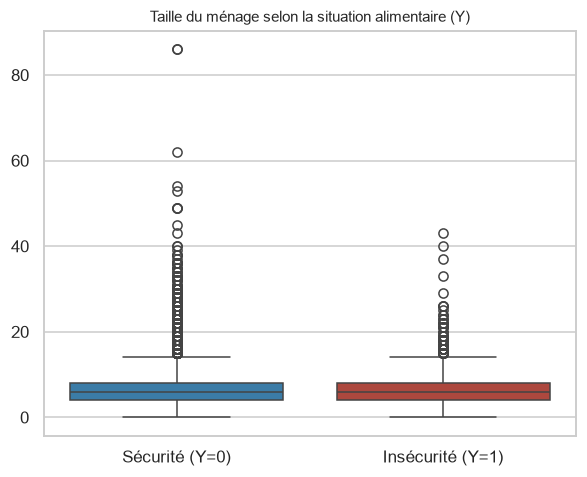
\includegraphics[width=0.5\textwidth]{outputs/bivarie_boxplot_taille.png}
\caption{Taille du ménage selon la situation alimentaire}
\label{fig:res-box-taille}
\end{figure}

\begin{figure}[H]
\centering
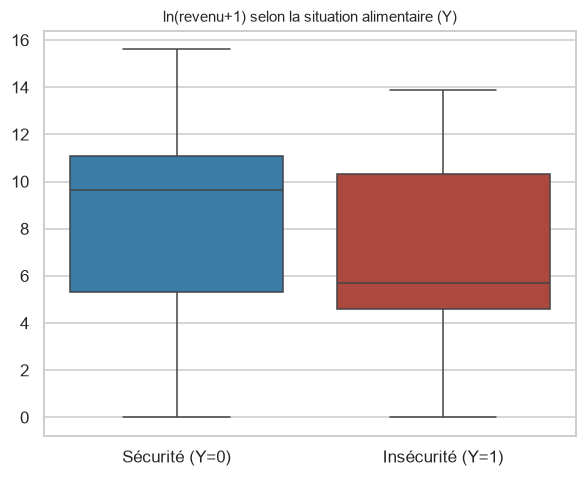
\includegraphics[width=0.5\textwidth]{outputs/bivarie_boxplot_revenu.png}
\caption{Revenu log-transformé selon la situation alimentaire}
\label{fig:res-box-revenu}
\end{figure}

\begin{figure}[H]
\centering
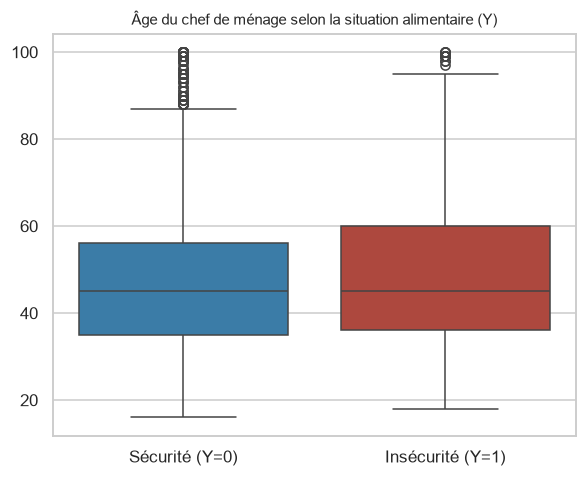
\includegraphics[width=0.5\textwidth]{outputs/bivarie_boxplot_age.png}
\caption{Âge du chef de ménage selon la situation alimentaire}
\label{fig:res-box-age}
\end{figure}

\begin{figure}[H]
\centering
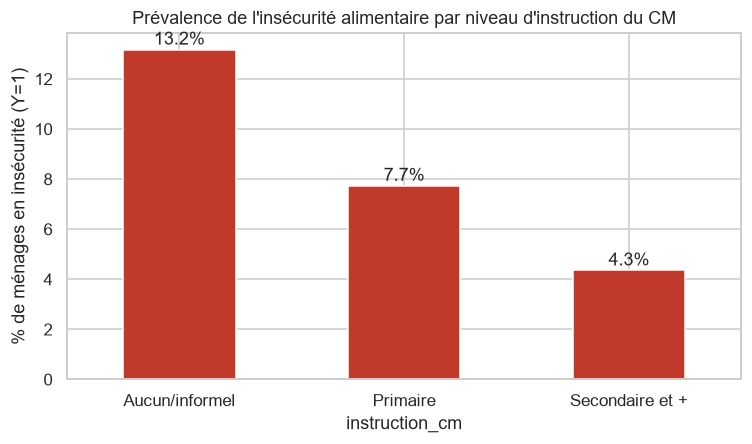
\includegraphics[width=0.62\textwidth]{outputs/bivarie_instruction.png}
\caption{Prévalence de l'insécurité alimentaire selon le niveau d'instruction du chef de ménage}
\label{fig:res-biv-instruction}
\end{figure}

\begin{figure}[H]
\centering
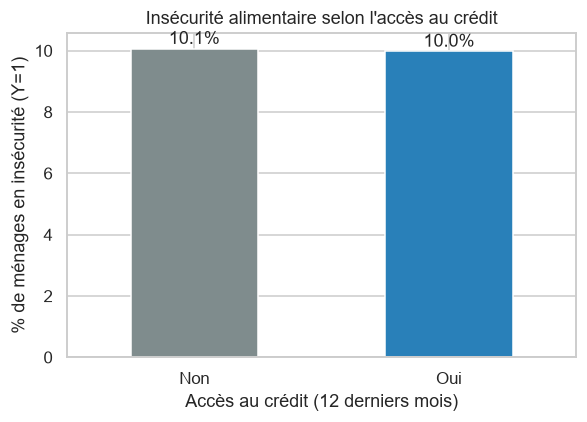
\includegraphics[width=0.5\textwidth]{outputs/bivarie_credit.png}
\caption{Prévalence de l'insécurité alimentaire selon l'accès au crédit}
\label{fig:res-biv-credit}
\end{figure}

\subsubsection{Tests bivariés étendus et correction pour comparaisons multiples}

L'analyse a été étendue à l'ensemble des variables indépendantes retenues
(Table~10 du chapitre~4), soit 22~tests, avec correction de Benjamini-Hochberg
(contrôle du \textsc{fdr}). Après correction, \textbf{20 des 22 variables
demeurent significativement associées} au statut alimentaire au seuil de
5\,\% ; seules la possession de bétail (\textsc{tlu}, $p_{aj} = 0{,}709$) et
l'accès au crédit ($p_{aj} = 0{,}908$) ne le sont pas. Les associations les
plus fortes concernent, par ordre de $p$-valeur ajustée croissante : les
dépenses alimentaires (log), l'accès à l'électricité ($V = 0{,}169$), le
département ($V = 0{,}179$), l'indice de qualité du logement, le niveau
d'instruction, le milieu de résidence ($V = 0{,}115$) et le revenu (log). La
nouvelle variable « mois de couverture des stocks » est également associée au
statut alimentaire ($p_{aj} < 0{,}001$), les ménages en insécurité déclarant
paradoxalement une couverture médiane plus longue (2~mois contre 0), reflet de
leur profil plus agricole.

\subsubsection{Multicolinéarité et linéarité dans le logit}

Aucune colinéarité problématique n'est détectée parmi les prédicteurs continus :
tous les \textsc{vif} sont inférieurs à 2 (maximum : diversification des
revenus, \textsc{vif} = 1,82). Pour les variables polytomiques, le \textsc{gvif}
de Fox et Monette conduit à la même conclusion
(Table~\ref{tab:res-gvif}) : la valeur normalisée maximale
$\text{GVIF}^{1/(2\,\text{ddl})} = 1{,}78$ (type de choc) reste sous le seuil
de $\sqrt{5} \approx 2{,}24$. L'ensemble des prédicteurs peut donc être
conservé dans le modèle logistique.

\begin{table}[H]
\centering
\caption{GVIF des variables polytomiques (Fox et Monette, 1992)}
\label{tab:res-gvif}
\begin{tabular}{lrrr}
\toprule
\textbf{Variable} & \textbf{ddl} & \textbf{GVIF} & \textbf{GVIF$^{1/(2\,\text{ddl})}$} \\
\midrule
Statut matrimonial    &  5 &   2,155 & 1,080 \\
Département           & 11 &   6,231 & 1,087 \\
Activité principale   &  5 &   5,163 & 1,178 \\
Type de choc          &  4 & 102,411 & 1,784 \\
\bottomrule
\end{tabular}
\end{table}

Le test de Box-Tidwell (Section~4.5.3) conclut à une linéarité acceptable dans
le logit pour l'âge ($p = 0{,}61$), la taille du ménage ($p = 0{,}21$) et le
ratio de dépendance ($p = 0{,}11$) ; seules les dépenses alimentaires (log)
présentent une non-linéarité significative ($p = 3{,}9\times10^{-18}$),
qu'avec $n \approx 15\,000$ il convient de relativiser et que les modèles
d'arbres (Random Forest, XGBoost), non paramétriques, capturent par
construction.

\subsubsection{Robustesse au plan de sondage : analyse pondérée design-based}
\label{sssec:res-ponderee}

Conformément à la Section~4.5.1, les statistiques descriptives et les tests
bivariés ont été recalculés en tenant compte du plan de sondage complexe
(poids \texttt{weight\_agvsa}, grappes en unités primaires, strates
reconstruites «~département~$\times$~milieu~») au moyen du package
\texttt{samplics} (linéarisation de Taylor). Les proportions et moyennes
pondérées sont assorties d'un intervalle de confiance design-based
(Table~\ref{tab:res-pondere-uni}). Pour les variables continues et binaires,
l'association avec $Y$ est testée par comparaison design-based des
moyennes/proportions par domaine ; pour les variables polytomiques, pour
lesquelles le test de Rao-Scott n'était pas exploitable dans la version
disponible du package, le test est calculé par repondération simple des
effectifs, conformément à la limite reconnue au chapitre~4.

\begin{table}[H]
\centering
\caption{Statistiques univariées pondérées design-based (intervalles de confiance
à 95\,\% de Taylor)}
\label{tab:res-pondere-uni}
\small\setlength{\tabcolsep}{5pt}
\begin{tabular}{llr}
\toprule
\textbf{Variable} & \textbf{Paramètre} & \textbf{Estimation [IC à 95\,\%]} \\
\midrule
Insécurité alimentaire ($Y=1$) & proportion & 9,66\,\% [8,98 ; 10,37] \\
Accès à l'électricité          & proportion & 41,62\,\% [39,49 ; 43,78] \\
Eau améliorée                  & proportion & 74,46\,\% [72,54 ; 76,30] \\
Accès au crédit                & proportion & 26,26\,\% [24,93 ; 27,64] \\
Résidence rurale               & proportion & 50,70\,\% [49,22 ; 52,17] \\
Taille du ménage               & moyenne    & 6,50 [6,40 ; 6,60] \\
Âge du chef de ménage          & moyenne    & 46,94 [46,58 ; 47,29] \\
$\ln(\text{revenu}+1)$         & moyenne    & 8,29 [8,15 ; 8,42] \\
\bottomrule
\end{tabular}
\end{table}

La prise en compte du plan de sondage \textbf{ne modifie pas les conclusions
qualitatives pour 20 des 22 variables} testées : les associations mises en
évidence au stade non pondéré (Section~\ref{ssec:res-bivarie}) demeurent
significatives en analyse pondérée. Deux variables font toutefois exception, ce
qui souligne l'intérêt de l'approche design-based :

\begin{itemize}
  \item la \textbf{possession de bétail} (\textsc{tlu}), non significative en
        non pondéré ($p = 0{,}68$), devient hautement significative en pondéré
        ($p = 4{,}4\times10^{-10}$) : l'élevage, concentré dans des strates du
        Nord fortement pondérées, apparaît alors nettement associé au statut
        alimentaire ;
  \item la \textbf{taille du ménage}, significative en non pondéré ($p = 0{,}006$),
        ne l'est plus en pondéré ($p = 0{,}159$) : l'écart observé sur
        l'échantillon brut ne résiste pas à la représentativité du plan de
        sondage.
\end{itemize}

Ces deux nuances mises à part, la convergence des deux approches conforte la
robustesse des associations décrites, et l'analyse pondérée fournit les
prévalences représentatives au niveau national mobilisées dans la discussion.

% ---------------------------------------------------------------------
\subsection{Déterminants du risque d'insécurité alimentaire (OS1)}
\label{ssec:res-os1}

La partition stratifiée 70/30 a produit un échantillon d'apprentissage de
10\,466 ménages (10,0\,\% de $Y=1$ ; 750~grappes) et un échantillon test de
4\,486 ménages (10,1\,\% ; 749~grappes). La régression logistique pénalisée
Elastic-Net ($\ell_1$-ratio~=~1,0, soit une pénalisation \textsc{lasso} pure ;
$C \approx 0{,}046$, sélectionnés par validation croisée) sert de modèle
prédictif ; l'inférence sur les déterminants repose sur
le \textsc{glm} binomial non pénalisé, pondéré par les poids d'enquête
normalisés, avec erreurs-types robustes en grappes (Section~4.5.3). La
Table~\ref{tab:res-or} présente les odds ratios significatifs au seuil de
5\,\%, classés en facteurs aggravants et protecteurs.

\begin{table}[H]
\centering
\caption{Déterminants significatifs de l'insécurité alimentaire — odds ratios du \textsc{glm}
binomial pondéré, erreurs-types robustes en grappes (échantillon d'apprentissage, $n = 10\,466$)}
\label{tab:res-or}
\begin{tabular}{lrrr}
\toprule
\textbf{Variable} & \textbf{OR} & \textbf{IC à 95\,\%} & \textbf{$p$-valeur} \\
\midrule
\multicolumn{4}{l}{\emph{Facteurs aggravants (OR $>$ 1)}} \\
\midrule
Vente d'actifs productifs (stratégie de crise) & 2,071 & [1,640 ; 2,615] & $<0{,}001$ \\
Département de l'Atacora (réf. : Atlantique)   & 2,285 & [1,451 ; 3,600] & $<0{,}001$ \\
Pratique de l'agriculture                      & 2,240 & [1,429 ; 3,512] & $<0{,}001$ \\
Assistance alimentaire reçue                   & 1,720 & [1,280 ; 2,313] & $<0{,}001$ \\
Taille du ménage (par personne suppl.)         & 1,031 & [1,010 ; 1,052] & 0,004 \\
\midrule
\multicolumn{4}{l}{\emph{Facteurs protecteurs (OR $<$ 1)}} \\
\midrule
Dépenses alimentaires (log)                    & 0,852 & [0,821 ; 0,883] & $<0{,}001$ \\
Accès à l'électricité                          & 0,495 & [0,385 ; 0,636] & $<0{,}001$ \\
Indice de qualité du logement (0--3)           & 0,805 & [0,734 ; 0,883] & $<0{,}001$ \\
Superficie emblavée (classe)                   & 0,840 & [0,777 ; 0,908] & $<0{,}001$ \\
Possession de bétail (\textsc{tlu})            & 0,929 & [0,895 ; 0,964] & $<0{,}001$ \\
Sécurité foncière                              & 0,666 & [0,502 ; 0,884] & 0,005 \\
Activité principale : commerce (réf. : agric.) & 0,630 & [0,457 ; 0,869] & 0,005 \\
Niveau d'instruction du CM (par niveau)        & 0,831 & [0,726 ; 0,951] & 0,007 \\
Taux de scolarisation des enfants              & 0,618 & [0,430 ; 0,889] & 0,009 \\
Département du Mono                            & 0,401 & [0,197 ; 0,816] & 0,012 \\
Toilettes améliorées                           & 0,697 & [0,525 ; 0,924] & 0,012 \\
Département de la Donga                        & 0,485 & [0,262 ; 0,895] & 0,021 \\
Département du Littoral                        & 0,442 & [0,209 ; 0,935] & 0,033 \\
Capacité de relèvement après choc              & 0,828 & [0,695 ; 0,988] & 0,036 \\
Diversification des revenus (par source)       & 0,823 & [0,686 ; 0,987] & 0,036 \\
Revenu mensuel (log)                           & 0,966 & [0,935 ; 0,999] & 0,041 \\
\bottomrule
\end{tabular}
\end{table}

Trois lectures se dégagent de ce tableau.

\textbf{Le capital physique et financier protège.} L'accès à l'électricité
divise par deux la cote d'insécurité (OR~=~0,495), et chaque point de l'indice
de qualité du logement la réduit de 20\,\% environ ; le niveau des dépenses
alimentaires, le revenu et la diversification des sources de revenus jouent
dans le même sens, de même que le capital humain (instruction du chef de
ménage, scolarisation des enfants) et le capital naturel sécurisé (superficie
emblavée, sécurité foncière, bétail).

\textbf{Les marqueurs de vulnérabilité en cours sont aggravants.} La vente
d'actifs productifs — stratégie d'adaptation destructrice — double la cote
d'insécurité (OR~=~2,071), signal de détresse plus que cause ; le lien positif
de l'assistance alimentaire reçue (OR~=~1,720) s'interprète de même comme un
effet de ciblage (l'aide va aux ménages déjà vulnérables) et non comme un effet
causal défavorable.

\textbf{La géographie demeure déterminante à caractéristiques contrôlées.}
Résider dans l'Atacora multiplie par 2,3 la cote d'insécurité par rapport à
l'Atlantique, alors même que les caractéristiques socio-économiques des ménages
sont contrôlées ; à l'inverse, le milieu rural en tant que tel n'est plus
significatif (OR~=~1,166 ; $p = 0{,}151$) une fois le département et les
conditions d'habitat pris en compte : l'effet « rural » observé au stade
bivarié transite par ces variables.

Au regard de l'hypothèse $H_1$, l'éducation du chef de ménage
(OR~=~0,831 ; $p = 0{,}007$) et la diversification des revenus
(OR~=~0,823 ; $p = 0{,}036$) sont confirmées comme déterminants significatifs.
En revanche, l'accès à l'eau améliorée, significatif au stade bivarié
($\chi^2$ ; $p_{aj} < 0{,}001$), ne l'est plus dans le modèle multivarié
(OR~=~0,831 ; $p = 0{,}070$), et la résidence rurale voit son effet absorbé par
le département : \textbf{$H_1$ est donc partiellement validée}.

\subsubsection{Qualité d'ajustement globale du modèle logistique}
\label{sssec:res-pseudor2}

Le modèle logistique ne disposant pas d'un $R^2$ au sens strict, trois
pseudo-$R^2$ complémentaires sont rapportés à partir des log-vraisemblances du
modèle complet $\ell(\hat\beta_{\text{complet}})$ et du modèle nul
$\ell(\hat\beta_{\text{nul}})$ (constante seule), conformément à la
Section~4.5.3. Le \textbf{pseudo-$R^2$ de McFadden} s'établit à \textbf{0,171},
valeur qui, sur l'échelle propre à cet indicateur (où l'intervalle 0,2--0,4
traduit déjà un très bon ajustement, à un niveau nettement inférieur à celui
d'un $R^2$ linéaire classique), dénote un ajustement satisfaisant. Les
pseudo-$R^2$ de \textbf{Cox et Snell} (0,103) et de \textbf{Nagelkerke} (0,219,
version normalisée corrigeant l'impossibilité pour le Cox-Snell d'atteindre~1)
confirment ce constat. Ces trois indicateurs sont étendus aux deux modèles
d'apprentissage à la Section~\ref{ssec:res-os2}
(Table~\ref{tab:res-pseudor2}) pour une comparaison de la qualité d'ajustement
globale entre les trois approches.

% ---------------------------------------------------------------------
\subsection{Comparaison des performances prédictives (OS2)}
\label{ssec:res-os2}

\subsubsection{Performances hors échantillon}

La Table~\ref{tab:res-perf} compare les trois modèles sur l'échantillon test
($n = 4\,486$), au seuil de classification de 0,5. Les courbes \textsc{roc}
correspondantes sont superposées à la Figure~\ref{fig:res-roc}, et les matrices
de confusion sont présentées séparément pour chaque modèle
(Figures~\ref{fig:res-cm-logit} à~\ref{fig:res-cm-xgb}).

\begin{table}[H]
\centering
\caption{Performances hors échantillon des trois modèles (échantillon test, $n = 4\,486$)}
\label{tab:res-perf}
\small\setlength{\tabcolsep}{4pt}
\begin{tabular}{lrrrrrrr}
\toprule
\textbf{Modèle} & \textbf{AUROC} & \textbf{IC à 95\,\%} & \textbf{Accur.} & \textbf{Recall} & \textbf{Préc.} & \textbf{F1} & \textbf{Brier} \\
\midrule
Régression Logistique & 0,773 & [0,750 ; 0,794] & 0,685 & 0,730 & 0,203 & 0,317 & 0,202 \\
Random Forest         & \textbf{0,801} & [0,780 ; 0,822] & 0,902 & 0,220 & 0,532 & 0,311 & 0,088 \\
XGBoost               & 0,794 & [0,773 ; 0,815] & 0,747 & 0,681 & 0,236 & 0,351 & 0,162 \\
\bottomrule
\end{tabular}
\end{table}

Les deux algorithmes d'apprentissage automatique dominent la régression
logistique sur le critère principal : les tests de DeLong concluent à une
différence d'\textsc{auroc} significative pour Random Forest contre Logit
($p < 0{,}0001$) comme pour XGBoost contre Logit ($p = 0{,}0005$), tandis que
XGBoost et Random Forest sont statistiquement équivalents ($p = 0{,}098$).
\textbf{L'hypothèse $H_2$ est ainsi confirmée} : les algorithmes de
\emph{machine learning} offrent une performance discriminante supérieure à
celle du modèle économétrique de référence, validée par le test de DeLong au
seuil de 5\,\%.

En application des critères de sélection de la Section~4.8.3 — \textsc{auroc}
maximale, puis, en cas d'équivalence statistique, \emph{recall} le plus élevé
compte tenu du coût social asymétrique du faux négatif — le critère primaire
place Random Forest en tête (0,801 contre 0,794), mais la différence n'étant
pas significative (DeLong, $p = 0{,}098$), le critère secondaire départage :
au seuil de 0,5, XGBoost identifie 68,1\,\% des ménages en insécurité contre
22,0\,\% seulement pour Random Forest, dont l'exactitude élevée (0,902)
masque un \emph{recall} effondré — profil inadapté à un objectif de détection
des ménages vulnérables. Le modèle \textbf{XGBoost est donc retenu comme
meilleur modèle}. Concrètement, sur les 451~ménages en insécurité de
l'échantillon test, XGBoost en détecte 307 (144~faux négatifs ;
Figure~\ref{fig:res-cm-xgb}).

\begin{figure}[H]
\centering
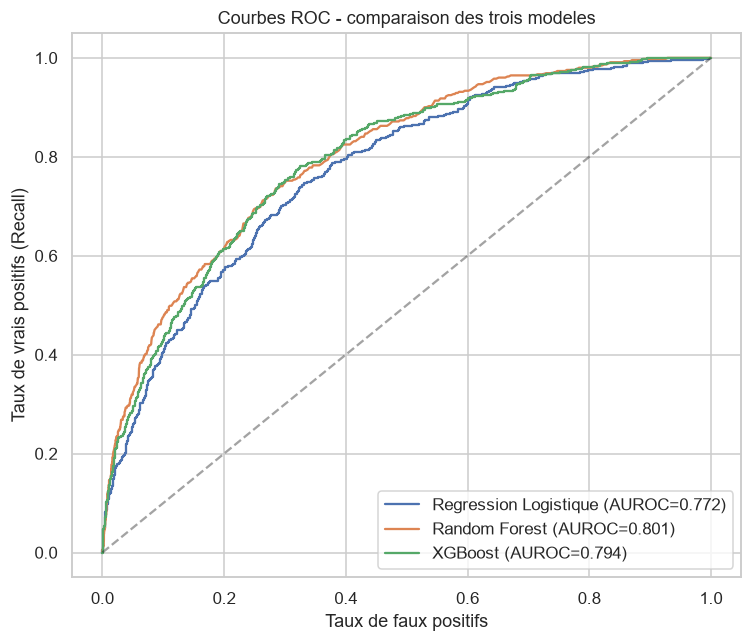
\includegraphics[width=0.62\textwidth]{outputs/courbes_roc.png}
\caption{Courbes \textsc{roc} des trois modèles (échantillon test)}
\label{fig:res-roc}
\end{figure}

\begin{figure}[H]
\centering
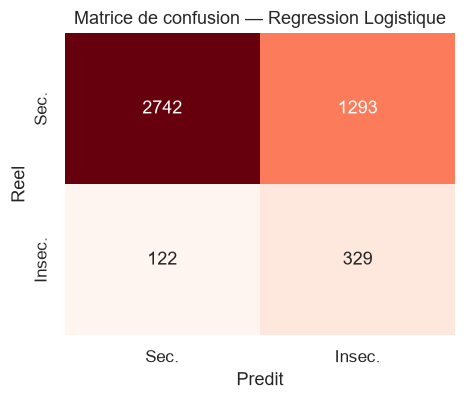
\includegraphics[width=0.45\textwidth]{outputs/matrice_confusion_regression_logistique.png}
\caption{Matrice de confusion de la Régression Logistique (seuil = 0,5)}
\label{fig:res-cm-logit}
\end{figure}

\begin{figure}[H]
\centering
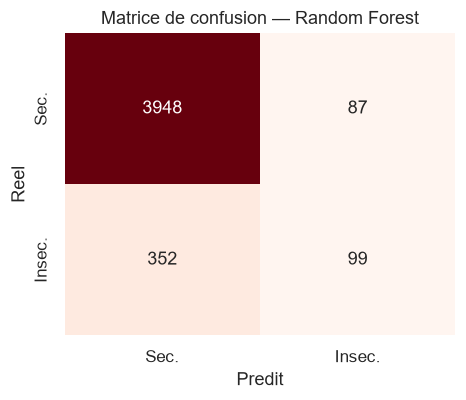
\includegraphics[width=0.45\textwidth]{outputs/matrice_confusion_random_forest.png}
\caption{Matrice de confusion du Random Forest (seuil = 0,5)}
\label{fig:res-cm-rf}
\end{figure}

\begin{figure}[H]
\centering
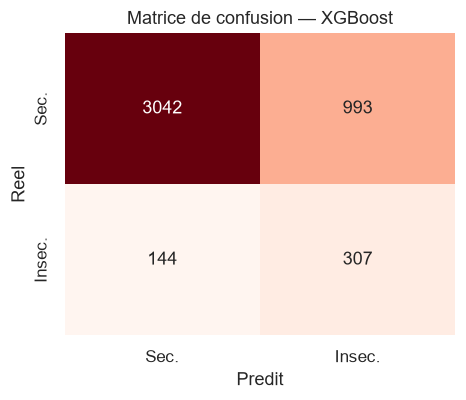
\includegraphics[width=0.45\textwidth]{outputs/matrice_confusion_xgboost.png}
\caption{Matrice de confusion du XGBoost (seuil = 0,5)}
\label{fig:res-cm-xgb}
\end{figure}

\subsubsection{Qualité d'ajustement globale : pseudo-$R^2$ des trois modèles}
\label{sssec:res-pseudor2-comp}

Les trois pseudo-$R^2$ introduits pour le Logit
(Section~\ref{sssec:res-pseudor2}) sont étendus aux deux modèles d'apprentissage
pour comparer la qualité d'ajustement globale des trois approches
(Table~\ref{tab:res-pseudor2}). Une précaution s'impose toutefois : le
\emph{class weighting} \textbf{décalibre volontairement} les probabilités
prédites (il optimise la discrimination, non la vraisemblance), de sorte qu'un
calcul direct sur les probabilités brutes des modèles d'ensemble produirait des
pseudo-$R^2$ négatifs, dénués de sens. Les valeurs inter-modèles sont donc
calculées sur des \textbf{probabilités recalibrées} (régression isotonique
ajustée sur une moitié de l'échantillon test, pseudo-$R^2$ évalué sur l'autre
moitié, sous-ensembles disjoints) ; la valeur classique \emph{in-sample} du
Logit (éq.~14) est rappelée en dernière ligne à titre de référence.

\begin{table}[H]
\centering
\caption{Pseudo-$R^2$ de qualité d'ajustement globale des trois modèles
(probabilités recalibrées sur l'échantillon test, sauf dernière ligne)}
\label{tab:res-pseudor2}
\begin{tabular}{lrrr}
\toprule
\textbf{Modèle} & \textbf{McFadden} & \textbf{Cox-Snell} & \textbf{Nagelkerke} \\
\midrule
Régression Logistique (test recalibré) & 0,147 & 0,091 & 0,191 \\
Random Forest (test recalibré)         & 0,181 & 0,111 & 0,232 \\
XGBoost (test recalibré)               & 0,174 & 0,107 & 0,224 \\
\midrule
Régression Logistique (\emph{in-sample}, éq.~14) & 0,171 & 0,103 & 0,219 \\
\bottomrule
\end{tabular}
\end{table}

Sur des probabilités remises sur un pied de comparabilité, les trois modèles
présentent une qualité d'ajustement globale du même ordre, le
\textbf{Random Forest} (McFadden~=~0,181) et le \textbf{XGBoost}
(0,174) devançant légèrement la régression logistique (0,147). L'ensemble des
pseudo-$R^2$ de McFadden se situe au voisinage du seuil de 0,2 usuellement
associé à un très bon ajustement pour cet indicateur, ce qui conforte, sous un
angle complémentaire à l'\textsc{auroc}, la pertinence des trois modèles et le
léger avantage des méthodes d'ensemble.

\subsubsection{Gestion du déséquilibre : \emph{class weighting} contre \textsc{smote}}

La comparaison prévue à la Section~4.5.2 conforte le choix du
\emph{class weighting} : à hyperparamètres identiques, le XGBoost entraîné sur
données suréchantillonnées par \textsc{smote} obtient une \textsc{auroc}
légèrement inférieure (0,783 contre 0,794) et surtout un \emph{recall}
effondré au seuil de 0,5 (0,118 contre 0,681), rédhibitoire au regard de
l'objectif de détection des ménages vulnérables. Le \emph{class weighting}
présente en outre l'avantage décisif de préserver l'intégration des poids
d'enquête, impossibles à attacher aux observations synthétiques de
\textsc{smote}.

\subsubsection{Analyse de sensibilité à la définition de la variable dépendante}

La hiérarchie des modèles est robuste à la définition de $Y$
(Section~4.2.4) : pour la définition de référence ($\{3,4\}$, prévalence
10,05\,\%) comme pour la définition élargie ($\{2,3,4\}$, 53,20\,\%),
XGBoost domine le Logit (0,794 contre 0,769 et 0,771 contre 0,749
respectivement). Seule la définition stricte ($\{4\}$, 0,83\,\% soit 124~cas)
inverse ponctuellement la hiérarchie (0,814 contre 0,831), inversion à
interpréter avec prudence compte tenu de l'instabilité d'une estimation fondée
sur si peu de cas positifs.

\subsubsection{Calibration des probabilités prédites}

Bruts, les trois modèles sont mal calibrés au sens du test de Hosmer-Lemeshow
($p < 0{,}001$ pour chacun), phénomène attendu : le \emph{class weighting}
optimise la discrimination au détriment de la justesse des probabilités. La
recalibration isotonique du modèle retenu (XGBoost), réalisée sur une moitié de
l'échantillon test et évaluée sur l'autre moitié, corrige ce défaut : le score
de Brier passe de 0,159 à \textbf{0,077} et le test de Hosmer-Lemeshow devient
non significatif ($p = 0{,}479$), indiquant une calibration adéquate
(Figure~\ref{fig:res-calibration}). Le modèle final — XGBoost recalibré — est
donc apte à produire des probabilités interprétables comme des risques réels,
condition posée par l'hypothèse $H_4$ pour le déploiement opérationnel.

\begin{figure}[H]
\centering
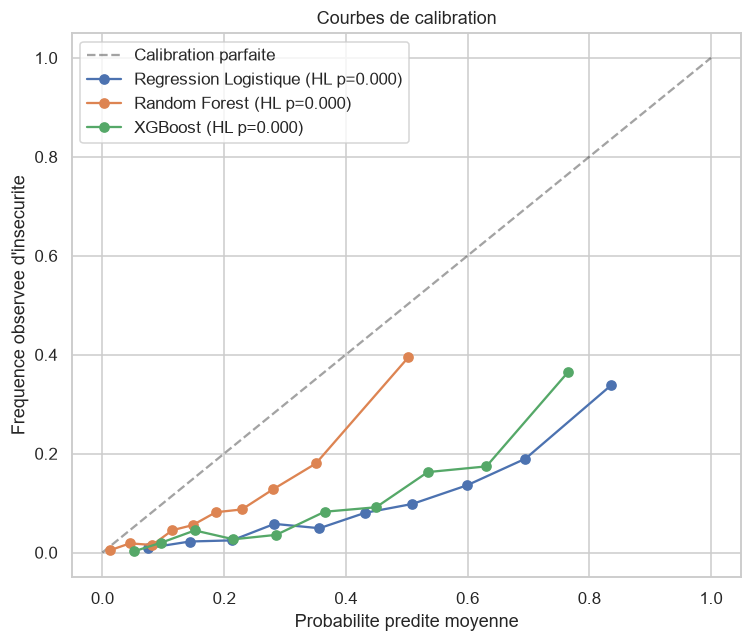
\includegraphics[width=0.62\textwidth]{outputs/calibration.png}
\caption{Courbes de calibration des trois modèles avant recalibration}
\label{fig:res-calibration}
\end{figure}

% ---------------------------------------------------------------------
\subsection{Interprétabilité du modèle retenu : valeurs \textsc{shap}}
\label{ssec:res-shap}

Conformément à la Section~4.7, les valeurs \textsc{shap} ont été calculées pour
les trois modèles (Tree\textsc{shap} pour Random Forest et XGBoost,
Linear\textsc{shap} pour le Logit), sur un échantillon de 1\,200 observations
de l'échantillon test.

\textbf{Importance globale.} Les classements d'importance
(Figure~\ref{fig:res-shap-imp}) convergent avec les déterminants identifiés en
OS1 : les dépenses alimentaires (log), l'accès à l'électricité et le revenu
(log) dominent, suivis de l'indice de qualité du logement et des variables
géographiques (département de l'Atacora). La convergence entre les trois
modèles — pourtant de familles algorithmiques différentes — renforce la
robustesse de ces conclusions.

\textbf{Direction des effets.} Le \emph{summary plot}
(Figure~\ref{fig:res-shap-summary}) confirme le sens des associations : des
dépenses alimentaires faibles, l'absence d'électricité, un revenu faible et un
logement précaire poussent la prédiction vers l'insécurité (valeurs
\textsc{shap} positives), tandis que les niveaux élevés de ces mêmes variables
sont protecteurs.

\textbf{Non-linéarités.} Les \emph{dependence plots} des trois variables les
plus importantes (Figures~\ref{fig:res-shap-dep1}
et~\ref{fig:res-shap-dep2}) révèlent notamment un effet de seuil des dépenses
alimentaires — la contribution au risque devient fortement positive sous un
plancher de dépenses — cohérent avec la non-linéarité détectée par le test de
Box-Tidwell (Section~\ref{ssec:res-bivarie}).

\textbf{Décomposition individuelle.} Les \emph{waterfall plots} de trois
ménages représentatifs illustrent l'usage opérationnel du modèle : pour le
ménage le plus à risque de l'échantillon (probabilité prédite de 0,91 ;
Figure~\ref{fig:res-shap-waterfall}), l'absence de dépenses alimentaires
déclarées (contribution $+0{,}90$ sur l'échelle logit), la résidence dans
l'Atacora ($+0{,}56$), un revenu très faible ($+0{,}16$), l'absence
d'électricité ($+0{,}16$) et l'assistance alimentaire reçue ($+0{,}15$)
constituent l'essentiel du diagnostic. Le
\emph{force plot} interactif du ménage médian, exporté en \textsc{html},
préfigure l'intégration de ces explications individuelles dans l'outil web
(OS4).

\begin{figure}[H]
\centering
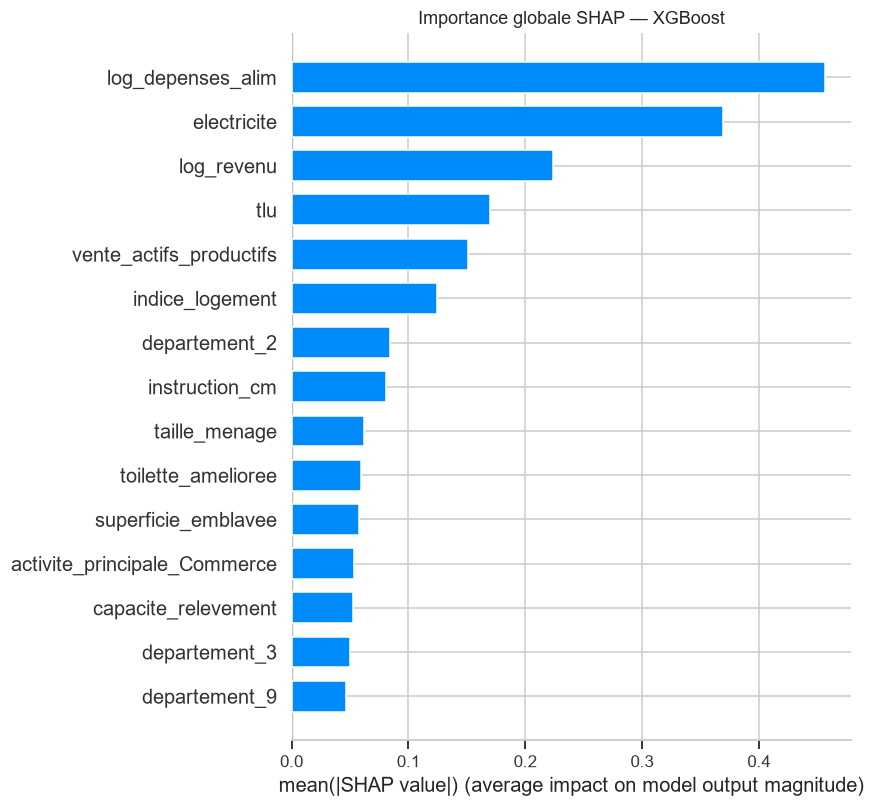
\includegraphics[width=0.72\textwidth]{outputs/shap_importance_xgboost.png}
\caption{Importance globale \textsc{shap} des prédicteurs — XGBoost}
\label{fig:res-shap-imp}
\end{figure}

\begin{figure}[H]
\centering
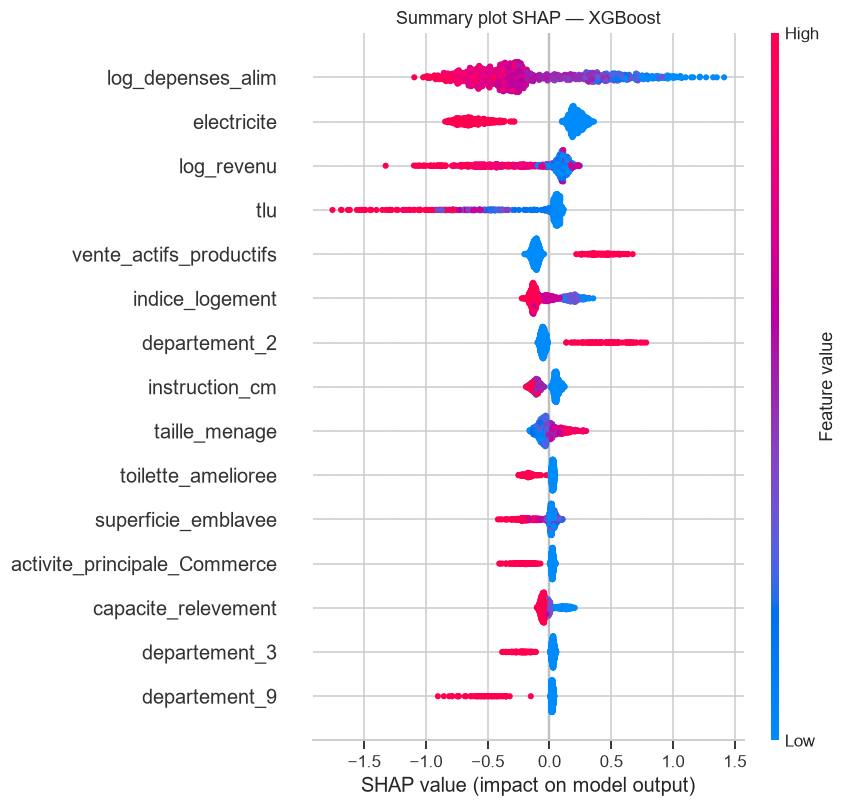
\includegraphics[width=0.72\textwidth]{outputs/shap_summary.png}
\caption{\emph{Summary plot} \textsc{shap} — importance et direction des effets (XGBoost)}
\label{fig:res-shap-summary}
\end{figure}

\begin{figure}[H]
\centering
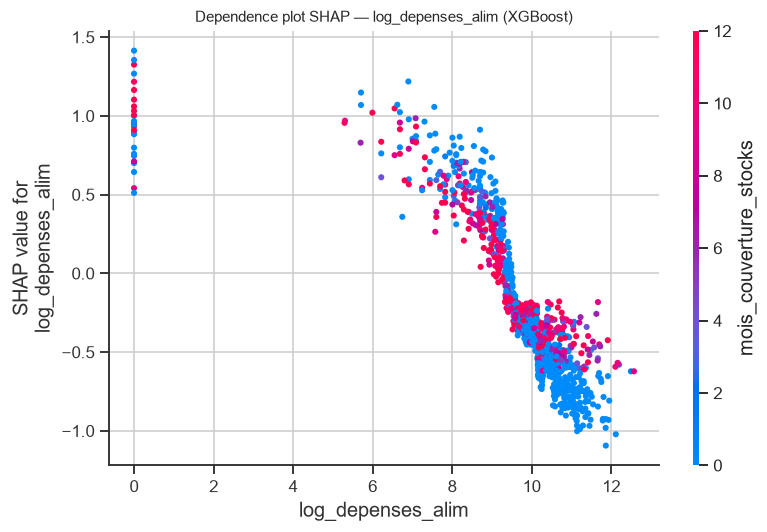
\includegraphics[width=0.6\textwidth]{outputs/shap_dependence_log_depenses_alim.png}
\caption{\emph{Dependence plot} \textsc{shap} des dépenses alimentaires (log)}
\label{fig:res-shap-dep1}
\end{figure}

\begin{figure}[H]
\centering
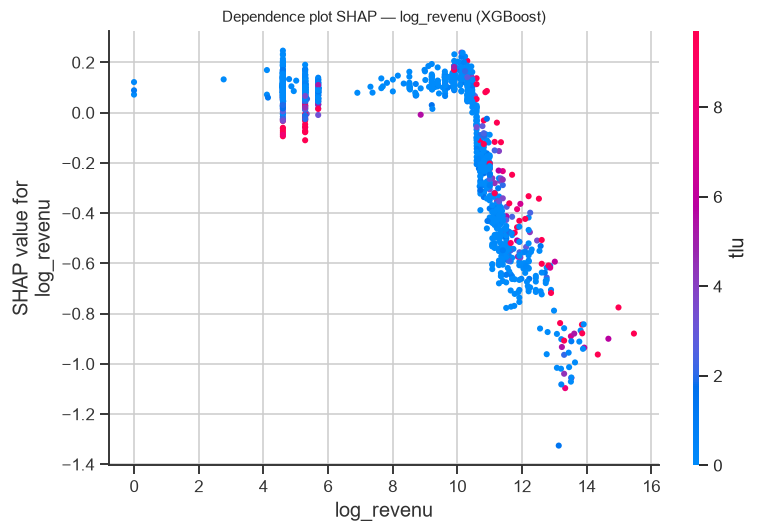
\includegraphics[width=0.6\textwidth]{outputs/shap_dependence_log_revenu.png}
\caption{\emph{Dependence plot} \textsc{shap} du revenu mensuel (log)}
\label{fig:res-shap-dep2}
\end{figure}

\begin{figure}[H]
\centering
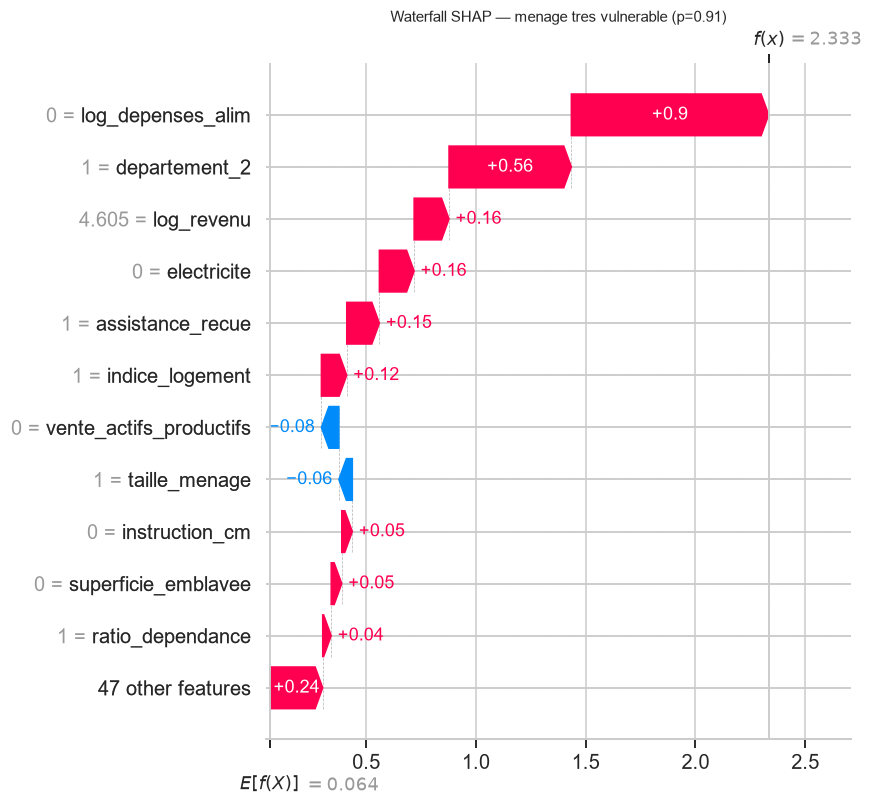
\includegraphics[width=0.72\textwidth]{outputs/shap_waterfall_menage_tres_vulnerable.png}
\caption{\emph{Waterfall plot} \textsc{shap} du ménage le plus vulnérable de l'échantillon
($\hat p = 0{,}91$)}
\label{fig:res-shap-waterfall}
\end{figure}

% ---------------------------------------------------------------------
\subsection{Cartographie communale du risque prédit (OS3)}
\label{ssec:res-os3}

Les probabilités individuelles prédites par le modèle final (XGBoost recalibré)
ont été agrégées par commune avec pondération par les poids d'enquête, puis
jointes au fond de carte des 77~communes (geoBoundaries \textsc{adm}2), avec un
appariement exhaustif (77/77).

\textbf{Autocorrélation spatiale.} L'indice de Moran calculé sur les risques
communaux moyens (matrice de contiguïté de type Queen, standardisée en ligne)
s'établit à $I = 0{,}570$ ($p = 0{,}001$, test par permutations), révélant une
autocorrélation spatiale positive forte et significative : les communes à
risque élevé sont géographiquement groupées. \textbf{L'hypothèse $H_3$ est
confirmée.}

\textbf{Poches de vulnérabilité.} La discrétisation de Jenks en quatre classes
(seuils : 0,08, 0,14 et 0,23) fait apparaître une poche principale de risque
très élevé dans le nord-ouest du pays (département de l'Atacora), et une poche
secondaire dans le centre-sud (Couffo et ouest du Zou)
(Figure~\ref{fig:res-carte}). Les dix communes au risque prédit le plus élevé
sont listées à la Table~\ref{tab:res-communes} : les cinq premières
appartiennent à l'Atacora, Boukoumbé et Toucountouna (39,3\,\% chacune) se
détachant nettement.

\begin{table}[H]
\centering
\caption{Les dix communes au risque prédit d'insécurité alimentaire le plus élevé}
\label{tab:res-communes}
\begin{tabular}{llr}
\toprule
\textbf{Commune} & \textbf{Département} & \textbf{Risque prédit moyen (\%)} \\
\midrule
Boukoumbé    & Atacora & 39,3 \\
Toucountouna & Atacora & 39,3 \\
Tanguiéta    & Atacora & 23,1 \\
Cobly        & Atacora & 22,5 \\
Matéri       & Atacora & 21,5 \\
Agbangnizoun & Zou     & 19,2 \\
Lalo         & Couffo  & 18,9 \\
Natitingou   & Atacora & 18,8 \\
Toviklin     & Couffo  & 17,8 \\
Djakotomey   & Couffo  & 17,4 \\
\bottomrule
\end{tabular}
\end{table}

\begin{figure}[H]
\centering
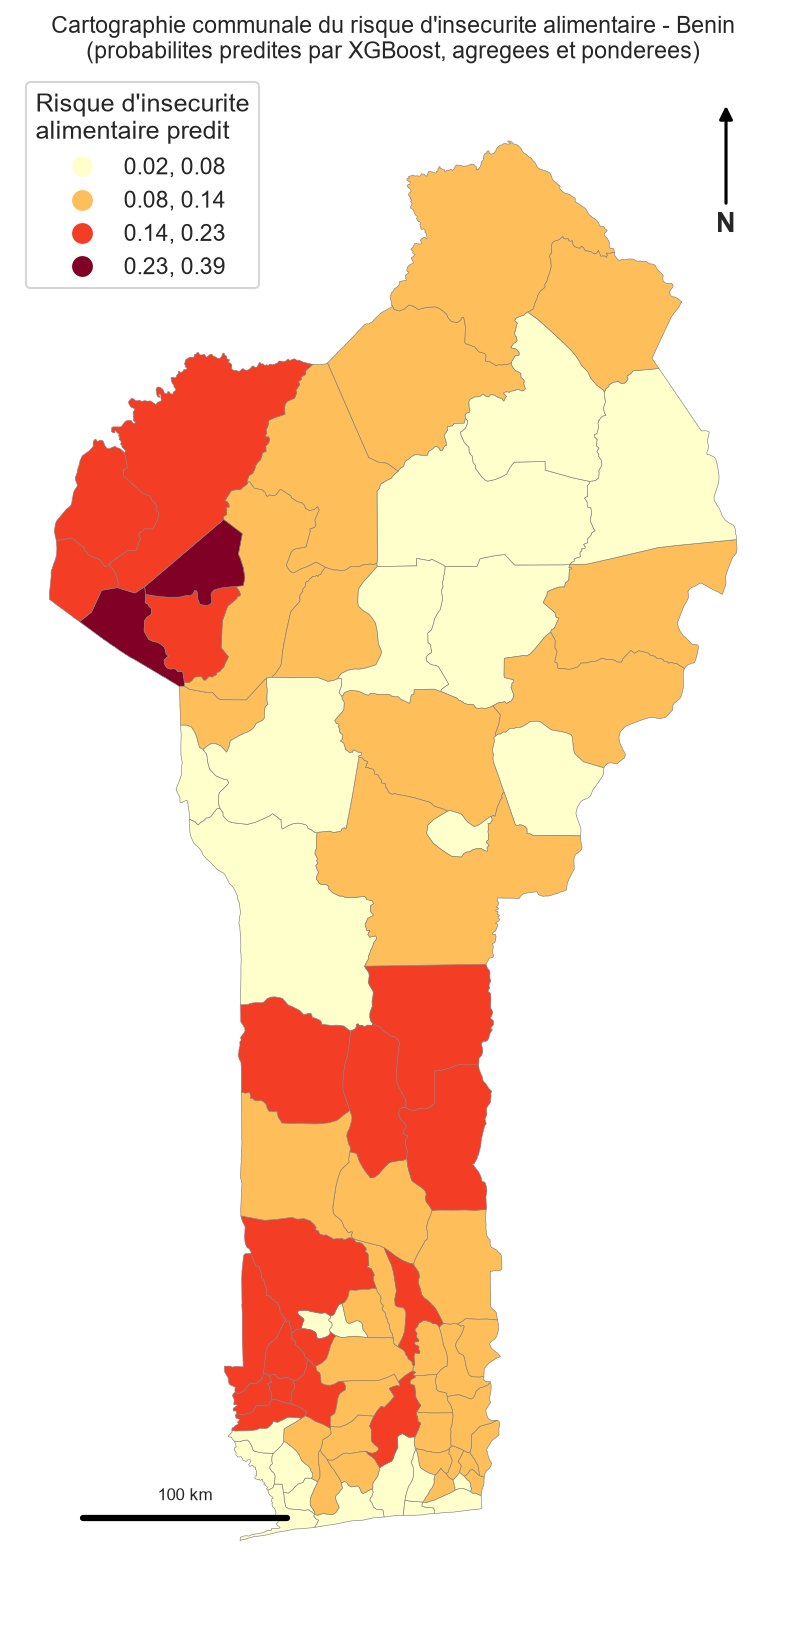
\includegraphics[width=0.8\textwidth]{outputs/carte_risque_communal.png}
\caption{Cartographie communale du risque prédit d'insécurité alimentaire au Bénin
(probabilités du modèle XGBoost, agrégées et pondérées ; discrétisation de Jenks, 4 classes)}
\label{fig:res-carte}
\end{figure}

Ce résultat cartographique converge avec la prévalence départementale observée
(Section~\ref{ssec:res-univarie}) tout en la raffinant à l'échelle communale :
au sein même de l'Atacora, le risque varie du simple au double entre communes,
information directement mobilisable pour le ciblage géographique des
interventions.

% ---------------------------------------------------------------------
\subsection{Produits opérationnels pour l'outil d'aide à la décision (OS4)}
\label{ssec:res-os4}

Le pipeline a produit les artefacts nécessaires au développement de l'outil
d'aide à la décision prévu par l'OS4 :

\begin{itemize}
  \item le \textbf{modèle final sérialisable} (XGBoost recalibré par régression
        isotonique), dont la calibration validée (Brier~=~0,077 ;
        Hosmer-Lemeshow $p = 0{,}479$) autorise des prédictions probabilistes
        fiables sur des ménages hors échantillon au profil similaire à celui de
        l'enquête — condition de l'hypothèse $H_4$ ;
  \item la \textbf{carte interactive} (\texttt{carte\_interactive.html},
        bibliothèque \texttt{folium}) offrant zoom et infobulles communales
        pour la consultation dynamique du risque ;
  \item le \textbf{force plot \textsc{shap} interactif}
        (\texttt{shap\_force\_menage\_median.html}) démontrant la faisabilité
        d'explications individuelles par ménage dans l'application ;
  \item l'\textbf{environnement logiciel figé}
        (\texttt{requirements\_versions.txt}, Section~4.10.1) garantissant la
        reproductibilité du déploiement.
\end{itemize}

Le développement de l'interface applicative elle-même relève des perspectives
et sera discuté au chapitre suivant.

% ---------------------------------------------------------------------
\subsection{Synthèse des résultats au regard des hypothèses de recherche}
\label{ssec:res-hypotheses}

La Table~\ref{tab:res-hypotheses} confronte les résultats obtenus aux quatre
hypothèses formulées au chapitre~2.

\begin{table}[H]
\centering
\caption{Confrontation des résultats aux hypothèses de recherche}
\label{tab:res-hypotheses}
\begin{tabular}{p{0.16\textwidth}p{0.5\textwidth}p{0.24\textwidth}}
\toprule
\textbf{Hypothèse} & \textbf{Résultat empirique} & \textbf{Verdict} \\
\midrule
$H_1$ (OS1) & Éducation (OR = 0,831 ; $p$ = 0,007) et diversification des
revenus (OR = 0,823 ; $p$ = 0,036) significatives ; eau améliorée et résidence
rurale significatives au stade bivarié mais non retenues par le modèle
multivarié (effets absorbés par l'habitat et le département). &
Partiellement validée \\
\addlinespace
$H_2$ (OS2) & AUROC : RF 0,801 $\approx$ XGBoost 0,794 $>$ Logit 0,773 ;
DeLong ML vs Logit significatif ($p \leq 5\times10^{-4}$) ; hiérarchie robuste
aux définitions de $Y$ (hors définition stricte, 124 cas). & Validée \\
\addlinespace
$H_3$ (OS3) & Indice de Moran $I$ = 0,570 ($p$ = 0,001) ; poches concentrées
dans l'Atacora (nord-ouest), secondairement Couffo--Zou. & Validée \\
\addlinespace
$H_4$ (OS4) & Après recalibration isotonique : Brier = 0,077 ;
Hosmer-Lemeshow $p$ = 0,479 ; artefacts opérationnels produits (carte et
explications interactives). & Validée \\
\bottomrule
\end{tabular}
\end{table}

En résumé, l'étude identifie un noyau robuste de déterminants — conditions
économiques du ménage (dépenses, revenu, diversification), capital humain
(instruction, scolarisation), habitat (électricité, qualité du logement) et
ancrage territorial (Atacora) — convergents entre l'approche économétrique
(odds ratios) et l'approche prédictive (valeurs \textsc{shap}) ; elle établit
la supériorité discriminante des algorithmes d'ensemble sur la régression
logistique, sélectionne et calibre un modèle XGBoost opérationnel, et localise
les poches communales de vulnérabilité qui fondent le ciblage géographique des
interventions. Ces résultats sont discutés et mis en perspective au chapitre
suivant.

% ===================== FIN DU CHAPITRE 5 =============================

% =====================================================================

\section{Présentation des résultats}
\label{sec:resultats}

Ce chapitre présente les résultats produits par le pipeline analytique décrit au
chapitre~4, exécuté sous \texttt{Python}~3.11 (\emph{notebook}
\texttt{Pipeline\_Insecurite\_Alimentaire\_Benin.ipynb}, graine aléatoire
\texttt{RANDOM\_STATE = 42}). La présentation suit la progression logique des
objectifs spécifiques : constitution et validation de la variable dépendante
(Section~\ref{ssec:res-echantillon}), analyse descriptive univariée et bivariée
(Sections~\ref{ssec:res-univarie} à~\ref{ssec:res-bivarie}), identification des
déterminants — OS1 (Section~\ref{ssec:res-os1}), comparaison des modèles
prédictifs — OS2 (Section~\ref{ssec:res-os2}), interprétabilité \textsc{shap}
(Section~\ref{ssec:res-shap}), cartographie communale du risque — OS3
(Section~\ref{ssec:res-os3}) et produits opérationnels pour l'outil d'aide à la
décision — OS4 (Section~\ref{ssec:res-os4}). Une synthèse confronte enfin les
résultats aux hypothèses de recherche (Section~\ref{ssec:res-hypotheses}).

% ---------------------------------------------------------------------
\subsection{Constitution de l'échantillon analytique et validation de la variable dépendante}
\label{ssec:res-echantillon}

\subsubsection{Échantillon analytique et prévalence de l'insécurité alimentaire}

La base AGVSAN 2017 compte 14\,952 ménages et 1\,406 variables. La variable
\texttt{Round\_INDICE\_SECAL} est renseignée pour la totalité des ménages :
aucune observation n'a été exclue et l'échantillon analytique est de
$n = 14\,952$. La Table~\ref{tab:res-repartition-y} présente la répartition des
quatre classes \textsc{cari} et les prévalences associées aux trois définitions
de la variable dépendante.

\begin{table}[H]
\centering
\caption{Répartition des classes \textsc{cari} et prévalence de $Y$ selon les trois définitions}
\label{tab:res-repartition-y}
\small\setlength{\tabcolsep}{4pt}
\begin{tabular}{lrr}
\toprule
\textbf{Classe \textsc{cari}} & \textbf{Effectif} & \textbf{\%} \\
\midrule
1 — Sécurité alimentaire          & 6\,998 & 46,80 \\
2 — Sécurité alimentaire limite   & 6\,452 & 43,15 \\
3 — Insécurité modérée            & 1\,378 &  9,22 \\
4 — Insécurité sévère             &    124 &  0,83 \\
\midrule
\textbf{Définition de $Y$}        & \textbf{Prévalence brute} & \textbf{Prévalence pondérée} \\
\midrule
Référence $\{3,4\}$               & 10,05\,\% & 9,66\,\% \\
Stricte $\{4\}$                   &  0,83\,\% & --- \\
Élargie $\{2,3,4\}$               & 53,20\,\% & --- \\
\bottomrule
\end{tabular}
\end{table}

Selon la définition de référence, 1\,502 ménages (10,05\,\% ; 9,66\,\% après
pondération par les poids d'enquête \texttt{weight\_agvsa}) sont en insécurité
alimentaire. Ce fort déséquilibre de classes justifie \emph{a posteriori} la
stratégie de \emph{class weighting} retenue au chapitre~4 (Section~4.5.2). La
prévalence pondérée est nettement différenciée selon le milieu de résidence :
13,03\,\% en milieu rural contre 6,19\,\% en milieu urbain (et 1,52\,\%
seulement à Cotonou), premier indice de la dimension territoriale du phénomène.

\subsubsection{Validation croisée de la classification officielle}

Conformément à la Section~4.2.4, le \textsc{sca} a été reconstruit de manière
indépendante à partir des 18~items bruts de consommation alimentaire
(moyenne~=~49,8 ; médiane~=~50,5 ; étendue 0--112). Sa répartition selon les
seuils standard du \textsc{pam} est : pauvre ($<28$) 1\,435 ménages (9,6\,\%),
limite (28--42) 3\,387 (22,7\,\%), acceptable ($>42$) 10\,130 (67,7\,\%). La
concordance entre le \textsc{sca} reconstruit dichotomisé
($\textsc{sca} \leq 42$) et la classification officielle dichotomisée s'établit
à \textbf{76,1\,\% d'accord global} avec un \textbf{Kappa de Cohen de 0,333},
et la corrélation ordinale entre le \textsc{sca} et la classe \textsc{cari} est
négative et hautement significative (Spearman $\rho = -0{,}371$ ;
$p < 0{,}001$), dans le sens attendu (un \textsc{sca} plus faible correspond à
une classe plus sévère). Cette concordance modérée est conforme à la
littérature : la classification \textsc{cari} officielle combine le \textsc{sca}
avec le \textsc{rcsi} et la part des dépenses alimentaires, de sorte qu'une
concordance parfaite avec le seul \textsc{sca} n'est pas attendue.

La validation par l'indice de stratégies de survie confirme la cohérence de la
variable dépendante : le \textsc{rcsi} moyen est de 18,96 chez les ménages en
insécurité contre 10,79 chez les ménages en sécurité (test unilatéral de
Mann-Whitney, $p = 2{,}2 \times 10^{-66}$).

\paragraph{Limite relative au \textsc{hfias}.} Le score \textsc{hfias} prévu
comme second indicateur de validation (Section~4.2.5) s'est révélé
\textbf{indisponible} dans la base ménage transmise (la colonne \texttt{Q\_9\_05}
du fichier correspond à un autre champ du questionnaire). La validation croisée
repose donc sur le seul \textsc{rcsi}, limite qui sera discutée au chapitre
suivant.

% ---------------------------------------------------------------------
\subsection{Analyse univariée des variables focales}
\label{ssec:res-univarie}

\subsubsection{Situation alimentaire des ménages}

Au niveau national, 89,95\,\% des ménages sont en sécurité alimentaire et
10,05\,\% en insécurité (90,34\,\% et 9,66\,\% après pondération ;
Figure~\ref{fig:res-y-national}). La stratification par département
(Figure~\ref{fig:res-y-departement}) révèle de fortes disparités : la
prévalence brute varie de 1,52\,\% dans le Littoral à \textbf{22,80\,\% dans
l'Atacora}, suivi du Couffo (16,40\,\%), des Collines (15,74\,\%) et du Zou
(11,63\,\%), tous au-dessus de la moyenne nationale. Cette hétérogénéité
géographique, déjà visible au stade descriptif, annonce les résultats de la
cartographie prédictive (Section~\ref{ssec:res-os3}).

\begin{figure}[H]
\centering
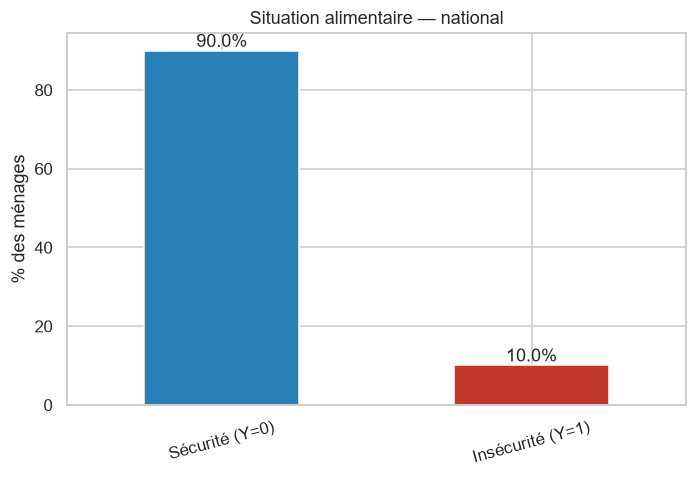
\includegraphics[width=0.62\textwidth]{outputs/univarie_Y_national.png}
\caption{Répartition nationale des ménages selon la situation alimentaire ($Y$)}
\label{fig:res-y-national}
\end{figure}

\begin{figure}[H]
\centering
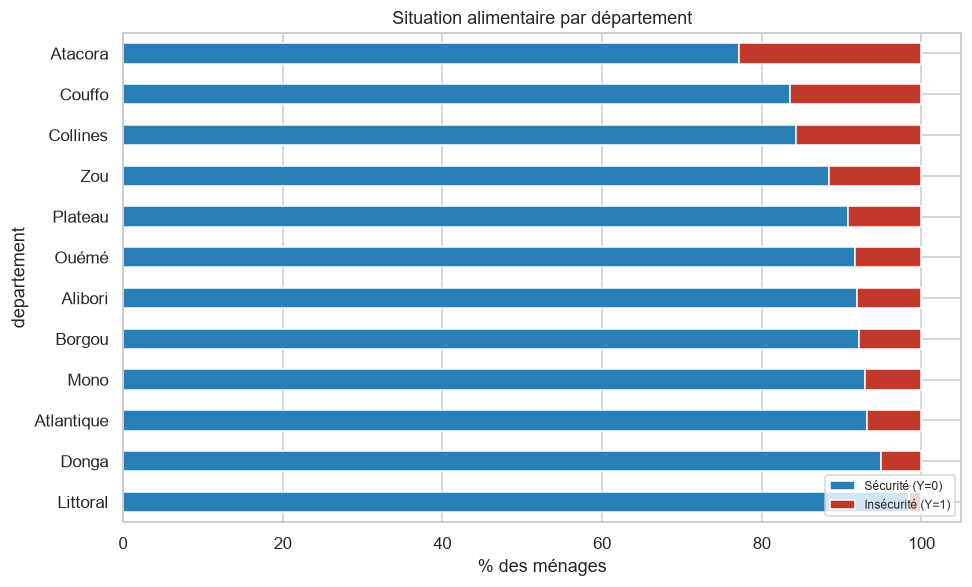
\includegraphics[width=0.85\textwidth]{outputs/univarie_Y_departement.png}
\caption{Situation alimentaire des ménages par département (barres empilées, \% en ligne)}
\label{fig:res-y-departement}
\end{figure}

\subsubsection{Taille des ménages}

La taille moyenne des ménages est de 6,83 personnes (médiane~=~6 ;
écart-type~=~4,57 ; CV~=~66,9\,\%), avec une distribution asymétrique à droite
(skewness~=~2,88) s'étirant jusqu'à 86 personnes
(Figure~\ref{fig:res-taille-hist}). Les ménages ruraux sont en moyenne plus
grands que les ménages urbains (7,2 contre 6,4 personnes ;
Figure~\ref{fig:res-taille-box}), les percentiles extrêmes confirmant cet écart
($P_{90}$ de 13 en milieu rural contre 11 en milieu urbain).

\begin{figure}[H]
\centering
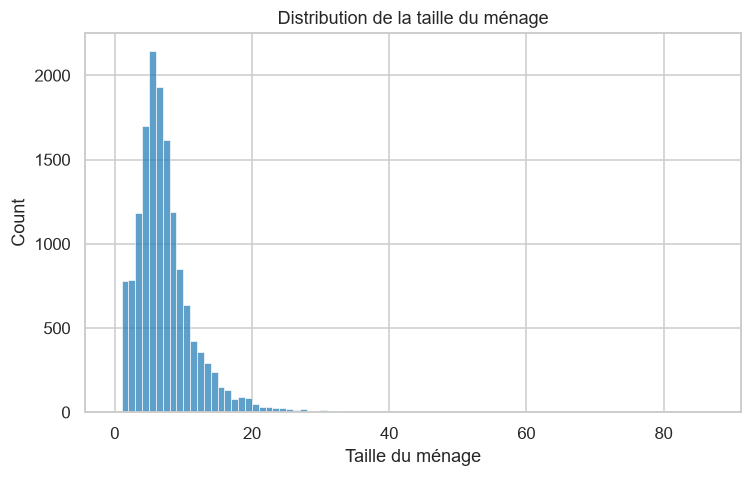
\includegraphics[width=0.62\textwidth]{outputs/univarie_taille_hist.png}
\caption{Distribution de la taille des ménages}
\label{fig:res-taille-hist}
\end{figure}

\begin{figure}[H]
\centering
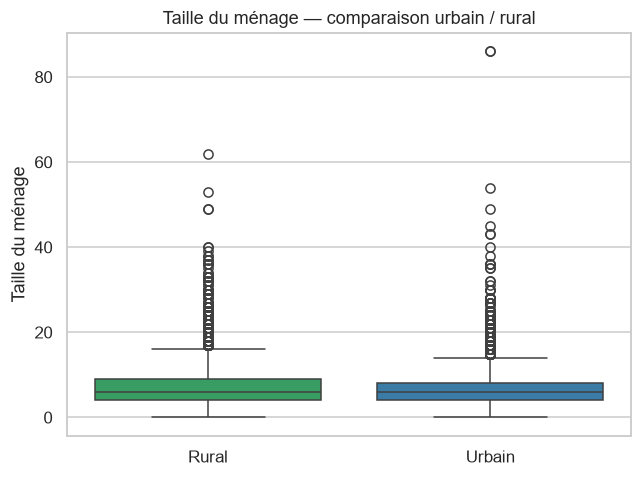
\includegraphics[width=0.55\textwidth]{outputs/univarie_taille_boxplot.png}
\caption{Taille des ménages : comparaison urbain / rural (boîtes à moustaches)}
\label{fig:res-taille-box}
\end{figure}

\subsubsection{Revenu mensuel}

Le revenu mensuel déclaré présente l'asymétrie extrême caractéristique des
données de revenu : moyenne de 68\,105 \textsc{fcfa} pour une médiane de
15\,000 \textsc{fcfa}, écart-type de 217\,941 \textsc{fcfa}
(CV~=~320\,\%), skewness de 11,06 et kurtosis de 181,8
(Figure~\ref{fig:res-revenu-brut}). La transformation logarithmique
$\ln(\text{revenu}+1)$ retenue pour la modélisation (Section~4.3.3) ramène la
skewness à $-0{,}06$, soit une distribution quasi symétrique
(Figure~\ref{fig:res-revenu-log}), ce qui valide empiriquement ce choix
méthodologique.

\begin{figure}[H]
\centering
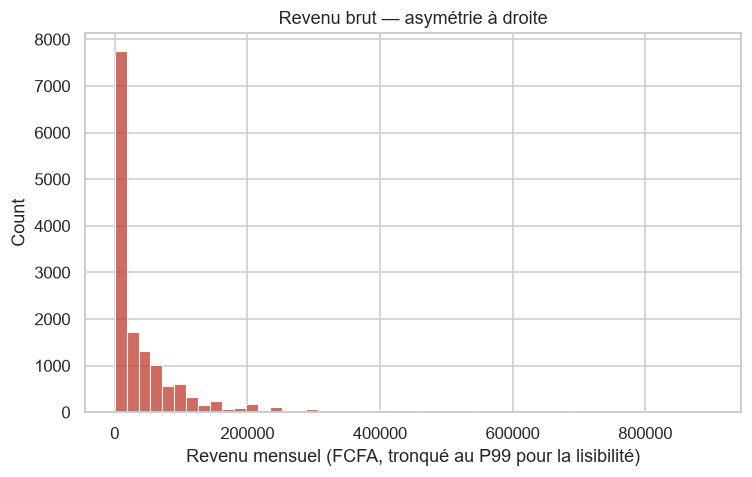
\includegraphics[width=0.62\textwidth]{outputs/univarie_revenu_brut.png}
\caption{Distribution du revenu mensuel brut (\textsc{fcfa}, tronqué au $P_{99}$)}
\label{fig:res-revenu-brut}
\end{figure}

\begin{figure}[H]
\centering
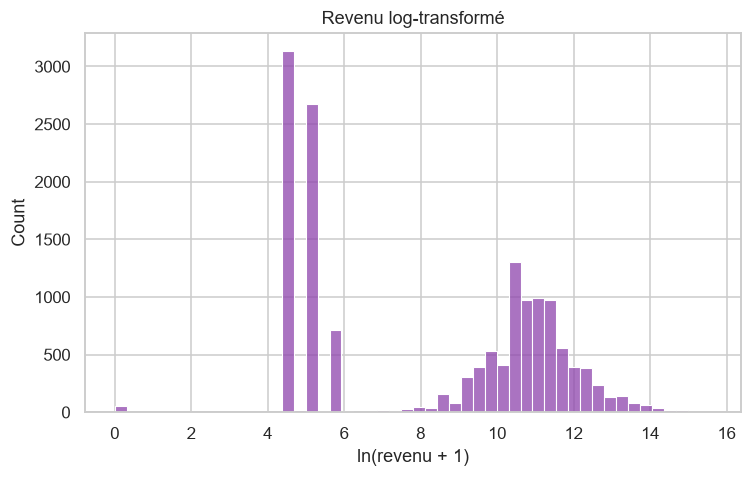
\includegraphics[width=0.62\textwidth]{outputs/univarie_revenu_log.png}
\caption{Distribution du revenu log-transformé $\ln(\text{revenu}+1)$}
\label{fig:res-revenu-log}
\end{figure}

\subsubsection{Âge du chef de ménage}

L'âge moyen du chef de ménage est de 47,1 ans (médiane~=~45 ;
écart-type~=~15,0 ; étendue 16--100 ans), avec une asymétrie modérée
(skewness~=~0,70 ; Figure~\ref{fig:res-age}). La répartition par tranches
usuelles est la suivante : moins de 30~ans, 8,94\,\% ; 30--44~ans, 37,22\,\% ;
45--59~ans, 32,30\,\% ; 60~ans et plus, 21,54\,\%.

\begin{figure}[H]
\centering
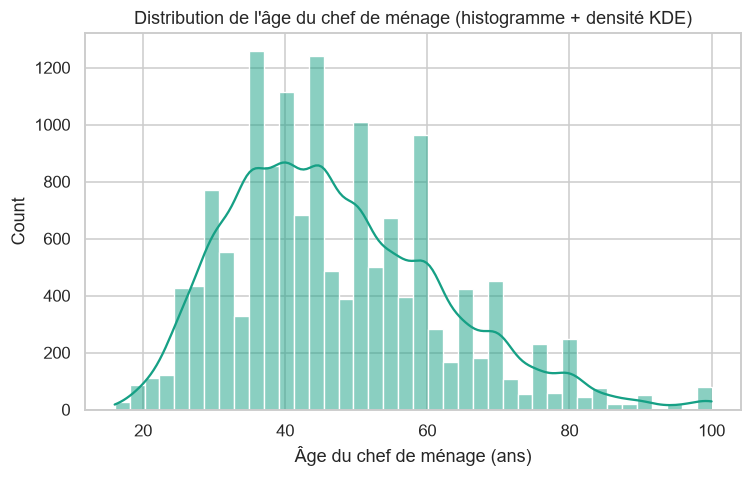
\includegraphics[width=0.62\textwidth]{outputs/univarie_age.png}
\caption{Distribution de l'âge du chef de ménage (histogramme et densité à noyau)}
\label{fig:res-age}
\end{figure}

\subsubsection{Niveau d'instruction du chef de ménage}

Plus de la moitié des chefs de ménage (51,22\,\%) n'ont aucune instruction
formelle ; viennent ensuite le primaire (22,59\,\%), le secondaire (17,04\,\%),
le supérieur (4,47\,\%), l'alphabétisation (3,36\,\%), l'école coranique
(1,17\,\%) et le cursus arabe (0,06\,\%) (Figure~\ref{fig:res-instruction}).
Après recodage en trois niveaux (Table~5 du chapitre~4), la répartition est :
\emph{Aucun/informel} 55,89\,\%, \emph{Primaire} 22,59\,\%,
\emph{Secondaire et plus} 21,52\,\%.

\begin{figure}[H]
\centering
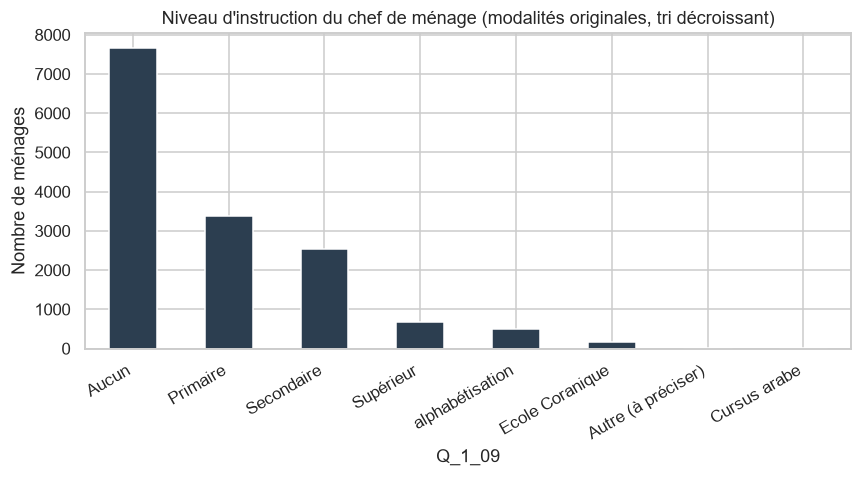
\includegraphics[width=0.72\textwidth]{outputs/univarie_instruction.png}
\caption{Niveau d'instruction du chef de ménage (modalités originales, tri décroissant)}
\label{fig:res-instruction}
\end{figure}

\subsubsection{Accès au crédit}

Un peu plus du quart des ménages (25,79\,\% ; 26,26\,\% pondéré) a contracté un
emprunt au cours des douze derniers mois. L'accès au crédit est légèrement plus
fréquent en milieu rural (27,31\,\%) qu'en milieu urbain (23,99\,\%)
(Figure~\ref{fig:res-credit-univ}).

\begin{figure}[H]
\centering
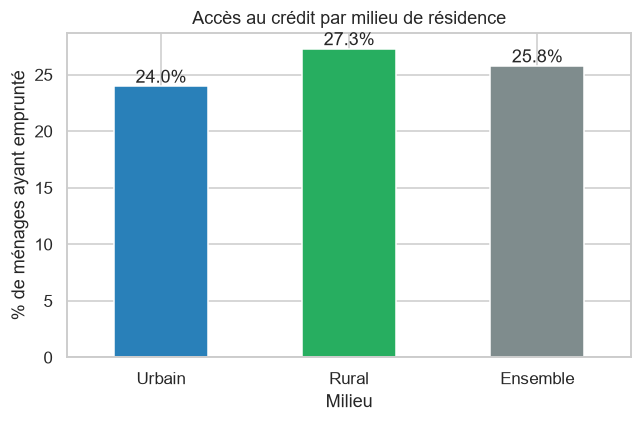
\includegraphics[width=0.55\textwidth]{outputs/univarie_credit.png}
\caption{Proportion de ménages ayant accès au crédit, par milieu de résidence}
\label{fig:res-credit-univ}
\end{figure}

% ---------------------------------------------------------------------
\subsection{Tests de normalité des variables continues}
\label{ssec:res-normalite}

La Table~\ref{tab:res-normalite} rapporte les tests de normalité prévus à la
Section~4.4.3. Pour les quatre variables continues focales, l'hypothèse de
normalité est rejetée par le test de Kolmogorov-Smirnov comme par celui de
Shapiro-Wilk ($p < 0{,}001$ dans tous les cas), conclusion corroborée par les
coefficients de forme et par les QQ-plots
(Figures~\ref{fig:res-qq-taille} et~\ref{fig:res-qq-age}). Conformément à la
règle de décision du chapitre~4 — et en tenant compte de la puissance très
élevée de ces tests avec $n \approx 15\,000$ — l'analyse bivariée recourt
systématiquement au test non paramétrique de Mann-Whitney pour les variables
continues.

\begin{table}[H]
\centering
\caption{Tests de normalité des variables continues focales ($n = 14\,952$)}
\label{tab:res-normalite}
\small\setlength{\tabcolsep}{4pt}
\begin{tabular}{lrrrrrl}
\toprule
\textbf{Variable} & \textbf{KS $D_n$} & \textbf{KS $p$} & \textbf{Shapiro $W$} & \textbf{Skew.} & \textbf{Kurt.} & \textbf{Conclusion} \\
\midrule
Taille du ménage        & 0,164 & $<0{,}001$ & 0,813 &  2,88 & 22,24  & Normalité rejetée \\
Revenu brut (\textsc{fcfa}) & 0,377 & $<0{,}001$ & 0,267 & 11,06 & 181,85 & Normalité rejetée \\
$\ln(\text{revenu}+1)$  & 0,239 & $<0{,}001$ & 0,848 & $-0{,}06$ & $-1{,}54$ & Normalité rejetée \\
Âge du chef de ménage   & 0,092 & $<0{,}001$ & 0,969 &  0,70 & 0,33   & Normalité rejetée \\
\bottomrule
\end{tabular}
\end{table}

\begin{figure}[H]
\centering
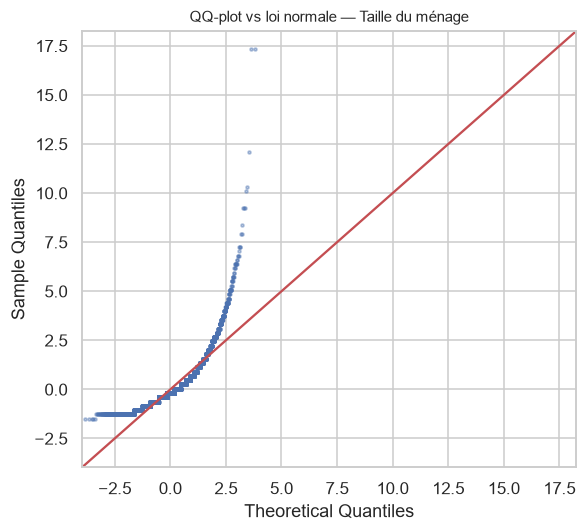
\includegraphics[width=0.48\textwidth]{outputs/normalite_qq_taille.png}
\caption{QQ-plot de la taille du ménage contre la loi normale standard}
\label{fig:res-qq-taille}
\end{figure}

\begin{figure}[H]
\centering
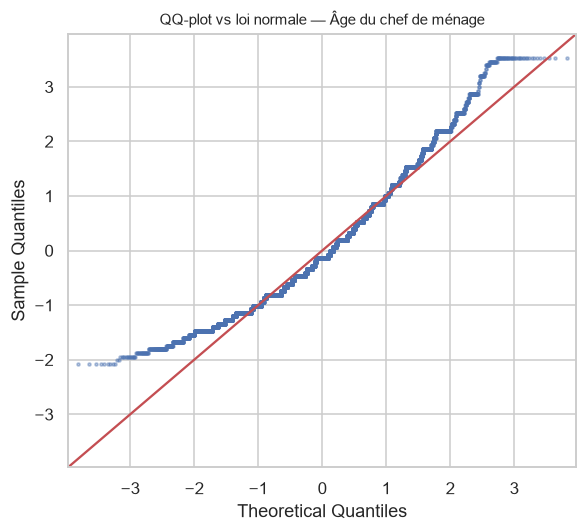
\includegraphics[width=0.48\textwidth]{outputs/normalite_qq_age.png}
\caption{QQ-plot de l'âge du chef de ménage contre la loi normale standard}
\label{fig:res-qq-age}
\end{figure}

% ---------------------------------------------------------------------
\subsection{Analyse bivariée et tests pré-estimation}
\label{ssec:res-bivarie}

\subsubsection{Variables focales croisées avec la situation alimentaire}

La Table~\ref{tab:res-bivarie-focales} synthétise les tests bivariés conduits
selon le canevas de la Section~4.4.4 (le test de Levene ayant orienté, avec le
rejet de la normalité, vers le test de Mann-Whitney pour les continues).

\begin{table}[H]
\centering
\caption{Analyse bivariée des variables focales $\times$ situation alimentaire ($Y$)}
\label{tab:res-bivarie-focales}
\small\setlength{\tabcolsep}{3.5pt}
\begin{tabular}{lllrl}
\toprule
\textbf{Variable} & \textbf{Test} & \textbf{Statistique} & \textbf{$p$-valeur} & \textbf{Conclusion} \\
\midrule
Taille du ménage        & Mann-Whitney & $U = 9\,667\,365{,}5$  & 0,006                 & Significatif \\
$\ln(\text{revenu}+1)$  & Mann-Whitney & $U = 8\,119\,697{,}0$  & $2{,}7\times10^{-36}$ & Significatif \\
Âge du chef de ménage   & Mann-Whitney & $U = 10\,613\,702{,}0$ & 0,001                 & Significatif \\
Niveau d'instruction    & $\chi^2$ (ddl = 2) & $\chi^2 = 226{,}06$ ; $V = 0{,}123$ & $8{,}2\times10^{-50}$ & Significatif \\
Accès au crédit         & $\chi^2$ (2$\times$2) & $\chi^2 = 0{,}013$ ; OR = 0,991 & 0,908 & \textbf{Non significatif} \\
\bottomrule
\end{tabular}
\end{table}

Quatre enseignements ressortent de cette analyse.

\textbf{(i) Le revenu est le facteur focal le plus discriminant.} Le revenu
log-transformé des ménages en insécurité est très inférieur à celui des ménages
en sécurité (médianes de 5,70 contre 9,63 sur l'échelle log, soit environ 297
contre 15\,198 \textsc{fcfa} sur l'échelle brute ;
$p = 2{,}7\times10^{-36}$ ; Figure~\ref{fig:res-box-revenu}), résultat cohérent
avec l'approche des pièges à pauvreté discutée au chapitre~3.

\textbf{(ii) Le gradient d'instruction est net et monotone.} La prévalence de
l'insécurité décroît régulièrement avec le niveau d'instruction du chef de
ménage : 13,17\,\% (\emph{Aucun/informel}), 7,73\,\% (\emph{Primaire}),
4,35\,\% (\emph{Secondaire et plus}) ($\chi^2(2) = 226{,}06$ ;
$V$ de Cramér~=~0,123 ; Figure~\ref{fig:res-biv-instruction}), conformément à
la littérature.

\textbf{(iii) Deux résultats vont à rebours de l'intuition.} D'une part, les
ménages en insécurité sont en moyenne légèrement \emph{plus petits} que les
ménages en sécurité (6,54 contre 6,87 personnes ; $p = 0{,}006$ ;
Figure~\ref{fig:res-box-taille}). D'autre part, la relation entre l'âge du chef
de ménage et l'insécurité est en U : la prévalence est plus élevée aux deux
extrémités de la distribution (11,23\,\% avant 30~ans et 12,79\,\% à 60~ans et
plus, contre 8,97\,\% et 9,13\,\% pour les tranches intermédiaires), les
moyennes différant significativement (48,69 contre 46,93 ans ; $p = 0{,}001$ ;
Figure~\ref{fig:res-box-age}).

\textbf{(iv) L'accès au crédit n'est pas associé au statut alimentaire.} La
prévalence de l'insécurité est quasi identique chez les ménages emprunteurs
(9,98\,\%) et non emprunteurs (10,07\,\%), et l'odds ratio brut est nul au sens
statistique (OR~=~0,991 ; IC à 95\,\% $[0{,}877\,;\,1{,}120]$ ; $p = 0{,}908$ ;
Figure~\ref{fig:res-biv-credit}). Ce résultat nul, contraire à l'hypothèse
d'un rôle protecteur du crédit, sera repris dans la discussion.

\begin{figure}[H]
\centering
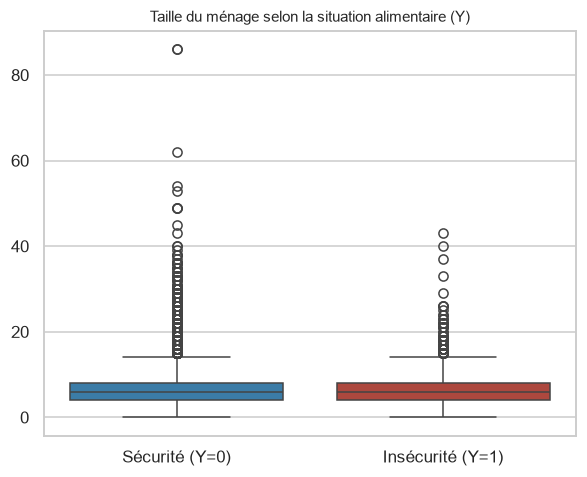
\includegraphics[width=0.5\textwidth]{outputs/bivarie_boxplot_taille.png}
\caption{Taille du ménage selon la situation alimentaire}
\label{fig:res-box-taille}
\end{figure}

\begin{figure}[H]
\centering
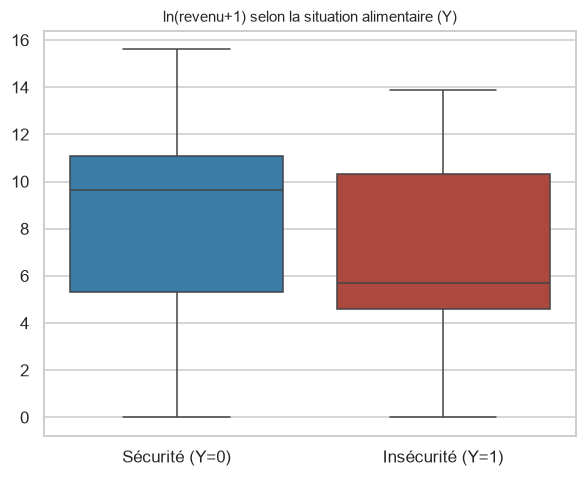
\includegraphics[width=0.5\textwidth]{outputs/bivarie_boxplot_revenu.png}
\caption{Revenu log-transformé selon la situation alimentaire}
\label{fig:res-box-revenu}
\end{figure}

\begin{figure}[H]
\centering
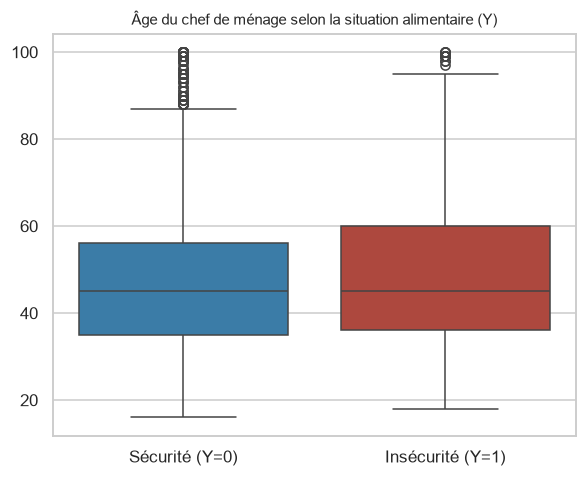
\includegraphics[width=0.5\textwidth]{outputs/bivarie_boxplot_age.png}
\caption{Âge du chef de ménage selon la situation alimentaire}
\label{fig:res-box-age}
\end{figure}

\begin{figure}[H]
\centering
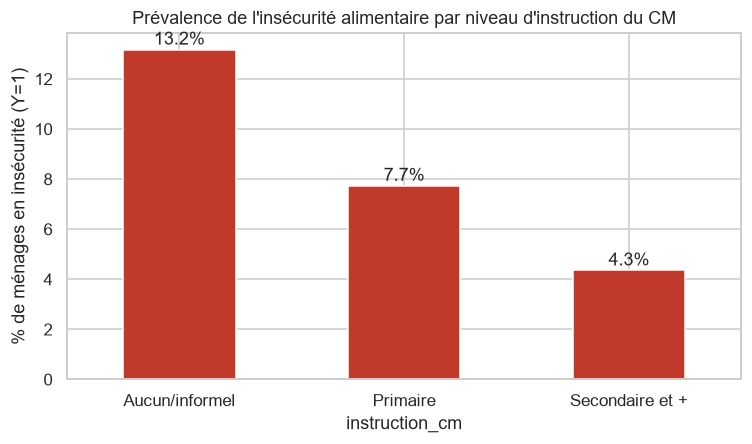
\includegraphics[width=0.62\textwidth]{outputs/bivarie_instruction.png}
\caption{Prévalence de l'insécurité alimentaire selon le niveau d'instruction du chef de ménage}
\label{fig:res-biv-instruction}
\end{figure}

\begin{figure}[H]
\centering
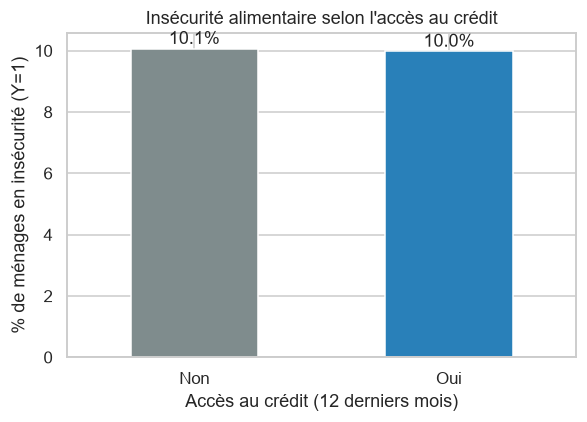
\includegraphics[width=0.5\textwidth]{outputs/bivarie_credit.png}
\caption{Prévalence de l'insécurité alimentaire selon l'accès au crédit}
\label{fig:res-biv-credit}
\end{figure}

\subsubsection{Tests bivariés étendus et correction pour comparaisons multiples}

L'analyse a été étendue à l'ensemble des variables indépendantes retenues
(Table~10 du chapitre~4), soit 22~tests, avec correction de Benjamini-Hochberg
(contrôle du \textsc{fdr}). Après correction, \textbf{20 des 22 variables
demeurent significativement associées} au statut alimentaire au seuil de
5\,\% ; seules la possession de bétail (\textsc{tlu}, $p_{aj} = 0{,}709$) et
l'accès au crédit ($p_{aj} = 0{,}908$) ne le sont pas. Les associations les
plus fortes concernent, par ordre de $p$-valeur ajustée croissante : les
dépenses alimentaires (log), l'accès à l'électricité ($V = 0{,}169$), le
département ($V = 0{,}179$), l'indice de qualité du logement, le niveau
d'instruction, le milieu de résidence ($V = 0{,}115$) et le revenu (log). La
nouvelle variable « mois de couverture des stocks » est également associée au
statut alimentaire ($p_{aj} < 0{,}001$), les ménages en insécurité déclarant
paradoxalement une couverture médiane plus longue (2~mois contre 0), reflet de
leur profil plus agricole.

\subsubsection{Multicolinéarité et linéarité dans le logit}

Aucune colinéarité problématique n'est détectée parmi les prédicteurs continus :
tous les \textsc{vif} sont inférieurs à 2 (maximum : diversification des
revenus, \textsc{vif} = 1,82). Pour les variables polytomiques, le \textsc{gvif}
de Fox et Monette conduit à la même conclusion
(Table~\ref{tab:res-gvif}) : la valeur normalisée maximale
$\text{GVIF}^{1/(2\,\text{ddl})} = 1{,}78$ (type de choc) reste sous le seuil
de $\sqrt{5} \approx 2{,}24$. L'ensemble des prédicteurs peut donc être
conservé dans le modèle logistique.

\begin{table}[H]
\centering
\caption{GVIF des variables polytomiques (Fox et Monette, 1992)}
\label{tab:res-gvif}
\begin{tabular}{lrrr}
\toprule
\textbf{Variable} & \textbf{ddl} & \textbf{GVIF} & \textbf{GVIF$^{1/(2\,\text{ddl})}$} \\
\midrule
Statut matrimonial    &  5 &   2,155 & 1,080 \\
Département           & 11 &   6,231 & 1,087 \\
Activité principale   &  5 &   5,163 & 1,178 \\
Type de choc          &  4 & 102,411 & 1,784 \\
\bottomrule
\end{tabular}
\end{table}

Le test de Box-Tidwell (Section~4.5.3) conclut à une linéarité acceptable dans
le logit pour l'âge ($p = 0{,}61$), la taille du ménage ($p = 0{,}21$) et le
ratio de dépendance ($p = 0{,}11$) ; seules les dépenses alimentaires (log)
présentent une non-linéarité significative ($p = 3{,}9\times10^{-18}$),
qu'avec $n \approx 15\,000$ il convient de relativiser et que les modèles
d'arbres (Random Forest, XGBoost), non paramétriques, capturent par
construction.

\subsubsection{Robustesse au plan de sondage : analyse pondérée design-based}
\label{sssec:res-ponderee}

Conformément à la Section~4.5.1, les statistiques descriptives et les tests
bivariés ont été recalculés en tenant compte du plan de sondage complexe
(poids \texttt{weight\_agvsa}, grappes en unités primaires, strates
reconstruites «~département~$\times$~milieu~») au moyen du package
\texttt{samplics} (linéarisation de Taylor). Les proportions et moyennes
pondérées sont assorties d'un intervalle de confiance design-based
(Table~\ref{tab:res-pondere-uni}). Pour les variables continues et binaires,
l'association avec $Y$ est testée par comparaison design-based des
moyennes/proportions par domaine ; pour les variables polytomiques, pour
lesquelles le test de Rao-Scott n'était pas exploitable dans la version
disponible du package, le test est calculé par repondération simple des
effectifs, conformément à la limite reconnue au chapitre~4.

\begin{table}[H]
\centering
\caption{Statistiques univariées pondérées design-based (intervalles de confiance
à 95\,\% de Taylor)}
\label{tab:res-pondere-uni}
\small\setlength{\tabcolsep}{5pt}
\begin{tabular}{llr}
\toprule
\textbf{Variable} & \textbf{Paramètre} & \textbf{Estimation [IC à 95\,\%]} \\
\midrule
Insécurité alimentaire ($Y=1$) & proportion & 9,66\,\% [8,98 ; 10,37] \\
Accès à l'électricité          & proportion & 41,62\,\% [39,49 ; 43,78] \\
Eau améliorée                  & proportion & 74,46\,\% [72,54 ; 76,30] \\
Accès au crédit                & proportion & 26,26\,\% [24,93 ; 27,64] \\
Résidence rurale               & proportion & 50,70\,\% [49,22 ; 52,17] \\
Taille du ménage               & moyenne    & 6,50 [6,40 ; 6,60] \\
Âge du chef de ménage          & moyenne    & 46,94 [46,58 ; 47,29] \\
$\ln(\text{revenu}+1)$         & moyenne    & 8,29 [8,15 ; 8,42] \\
\bottomrule
\end{tabular}
\end{table}

La prise en compte du plan de sondage \textbf{ne modifie pas les conclusions
qualitatives pour 20 des 22 variables} testées : les associations mises en
évidence au stade non pondéré (Section~\ref{ssec:res-bivarie}) demeurent
significatives en analyse pondérée. Deux variables font toutefois exception, ce
qui souligne l'intérêt de l'approche design-based :

\begin{itemize}
  \item la \textbf{possession de bétail} (\textsc{tlu}), non significative en
        non pondéré ($p = 0{,}68$), devient hautement significative en pondéré
        ($p = 4{,}4\times10^{-10}$) : l'élevage, concentré dans des strates du
        Nord fortement pondérées, apparaît alors nettement associé au statut
        alimentaire ;
  \item la \textbf{taille du ménage}, significative en non pondéré ($p = 0{,}006$),
        ne l'est plus en pondéré ($p = 0{,}159$) : l'écart observé sur
        l'échantillon brut ne résiste pas à la représentativité du plan de
        sondage.
\end{itemize}

Ces deux nuances mises à part, la convergence des deux approches conforte la
robustesse des associations décrites, et l'analyse pondérée fournit les
prévalences représentatives au niveau national mobilisées dans la discussion.

% ---------------------------------------------------------------------
\subsection{Déterminants du risque d'insécurité alimentaire (OS1)}
\label{ssec:res-os1}

La partition stratifiée 70/30 a produit un échantillon d'apprentissage de
10\,466 ménages (10,0\,\% de $Y=1$ ; 750~grappes) et un échantillon test de
4\,486 ménages (10,1\,\% ; 749~grappes). La régression logistique pénalisée
Elastic-Net ($\ell_1$-ratio~=~1,0, soit une pénalisation \textsc{lasso} pure ;
$C \approx 0{,}046$, sélectionnés par validation croisée) sert de modèle
prédictif ; l'inférence sur les déterminants repose sur
le \textsc{glm} binomial non pénalisé, pondéré par les poids d'enquête
normalisés, avec erreurs-types robustes en grappes (Section~4.5.3). La
Table~\ref{tab:res-or} présente les odds ratios significatifs au seuil de
5\,\%, classés en facteurs aggravants et protecteurs.

\begin{table}[H]
\centering
\caption{Déterminants significatifs de l'insécurité alimentaire — odds ratios du \textsc{glm}
binomial pondéré, erreurs-types robustes en grappes (échantillon d'apprentissage, $n = 10\,466$)}
\label{tab:res-or}
\begin{tabular}{lrrr}
\toprule
\textbf{Variable} & \textbf{OR} & \textbf{IC à 95\,\%} & \textbf{$p$-valeur} \\
\midrule
\multicolumn{4}{l}{\emph{Facteurs aggravants (OR $>$ 1)}} \\
\midrule
Vente d'actifs productifs (stratégie de crise) & 2,071 & [1,640 ; 2,615] & $<0{,}001$ \\
Département de l'Atacora (réf. : Atlantique)   & 2,285 & [1,451 ; 3,600] & $<0{,}001$ \\
Pratique de l'agriculture                      & 2,240 & [1,429 ; 3,512] & $<0{,}001$ \\
Assistance alimentaire reçue                   & 1,720 & [1,280 ; 2,313] & $<0{,}001$ \\
Taille du ménage (par personne suppl.)         & 1,031 & [1,010 ; 1,052] & 0,004 \\
\midrule
\multicolumn{4}{l}{\emph{Facteurs protecteurs (OR $<$ 1)}} \\
\midrule
Dépenses alimentaires (log)                    & 0,852 & [0,821 ; 0,883] & $<0{,}001$ \\
Accès à l'électricité                          & 0,495 & [0,385 ; 0,636] & $<0{,}001$ \\
Indice de qualité du logement (0--3)           & 0,805 & [0,734 ; 0,883] & $<0{,}001$ \\
Superficie emblavée (classe)                   & 0,840 & [0,777 ; 0,908] & $<0{,}001$ \\
Possession de bétail (\textsc{tlu})            & 0,929 & [0,895 ; 0,964] & $<0{,}001$ \\
Sécurité foncière                              & 0,666 & [0,502 ; 0,884] & 0,005 \\
Activité principale : commerce (réf. : agric.) & 0,630 & [0,457 ; 0,869] & 0,005 \\
Niveau d'instruction du CM (par niveau)        & 0,831 & [0,726 ; 0,951] & 0,007 \\
Taux de scolarisation des enfants              & 0,618 & [0,430 ; 0,889] & 0,009 \\
Département du Mono                            & 0,401 & [0,197 ; 0,816] & 0,012 \\
Toilettes améliorées                           & 0,697 & [0,525 ; 0,924] & 0,012 \\
Département de la Donga                        & 0,485 & [0,262 ; 0,895] & 0,021 \\
Département du Littoral                        & 0,442 & [0,209 ; 0,935] & 0,033 \\
Capacité de relèvement après choc              & 0,828 & [0,695 ; 0,988] & 0,036 \\
Diversification des revenus (par source)       & 0,823 & [0,686 ; 0,987] & 0,036 \\
Revenu mensuel (log)                           & 0,966 & [0,935 ; 0,999] & 0,041 \\
\bottomrule
\end{tabular}
\end{table}

Trois lectures se dégagent de ce tableau.

\textbf{Le capital physique et financier protège.} L'accès à l'électricité
divise par deux la cote d'insécurité (OR~=~0,495), et chaque point de l'indice
de qualité du logement la réduit de 20\,\% environ ; le niveau des dépenses
alimentaires, le revenu et la diversification des sources de revenus jouent
dans le même sens, de même que le capital humain (instruction du chef de
ménage, scolarisation des enfants) et le capital naturel sécurisé (superficie
emblavée, sécurité foncière, bétail).

\textbf{Les marqueurs de vulnérabilité en cours sont aggravants.} La vente
d'actifs productifs — stratégie d'adaptation destructrice — double la cote
d'insécurité (OR~=~2,071), signal de détresse plus que cause ; le lien positif
de l'assistance alimentaire reçue (OR~=~1,720) s'interprète de même comme un
effet de ciblage (l'aide va aux ménages déjà vulnérables) et non comme un effet
causal défavorable.

\textbf{La géographie demeure déterminante à caractéristiques contrôlées.}
Résider dans l'Atacora multiplie par 2,3 la cote d'insécurité par rapport à
l'Atlantique, alors même que les caractéristiques socio-économiques des ménages
sont contrôlées ; à l'inverse, le milieu rural en tant que tel n'est plus
significatif (OR~=~1,166 ; $p = 0{,}151$) une fois le département et les
conditions d'habitat pris en compte : l'effet « rural » observé au stade
bivarié transite par ces variables.

Au regard de l'hypothèse $H_1$, l'éducation du chef de ménage
(OR~=~0,831 ; $p = 0{,}007$) et la diversification des revenus
(OR~=~0,823 ; $p = 0{,}036$) sont confirmées comme déterminants significatifs.
En revanche, l'accès à l'eau améliorée, significatif au stade bivarié
($\chi^2$ ; $p_{aj} < 0{,}001$), ne l'est plus dans le modèle multivarié
(OR~=~0,831 ; $p = 0{,}070$), et la résidence rurale voit son effet absorbé par
le département : \textbf{$H_1$ est donc partiellement validée}.

\subsubsection{Qualité d'ajustement globale du modèle logistique}
\label{sssec:res-pseudor2}

Le modèle logistique ne disposant pas d'un $R^2$ au sens strict, trois
pseudo-$R^2$ complémentaires sont rapportés à partir des log-vraisemblances du
modèle complet $\ell(\hat\beta_{\text{complet}})$ et du modèle nul
$\ell(\hat\beta_{\text{nul}})$ (constante seule), conformément à la
Section~4.5.3. Le \textbf{pseudo-$R^2$ de McFadden} s'établit à \textbf{0,171},
valeur qui, sur l'échelle propre à cet indicateur (où l'intervalle 0,2--0,4
traduit déjà un très bon ajustement, à un niveau nettement inférieur à celui
d'un $R^2$ linéaire classique), dénote un ajustement satisfaisant. Les
pseudo-$R^2$ de \textbf{Cox et Snell} (0,103) et de \textbf{Nagelkerke} (0,219,
version normalisée corrigeant l'impossibilité pour le Cox-Snell d'atteindre~1)
confirment ce constat. Ces trois indicateurs sont étendus aux deux modèles
d'apprentissage à la Section~\ref{ssec:res-os2}
(Table~\ref{tab:res-pseudor2}) pour une comparaison de la qualité d'ajustement
globale entre les trois approches.

% ---------------------------------------------------------------------
\subsection{Comparaison des performances prédictives (OS2)}
\label{ssec:res-os2}

\subsubsection{Performances hors échantillon}

La Table~\ref{tab:res-perf} compare les trois modèles sur l'échantillon test
($n = 4\,486$), au seuil de classification de 0,5. Les courbes \textsc{roc}
correspondantes sont superposées à la Figure~\ref{fig:res-roc}, et les matrices
de confusion sont présentées séparément pour chaque modèle
(Figures~\ref{fig:res-cm-logit} à~\ref{fig:res-cm-xgb}).

\begin{table}[H]
\centering
\caption{Performances hors échantillon des trois modèles (échantillon test, $n = 4\,486$)}
\label{tab:res-perf}
\small\setlength{\tabcolsep}{4pt}
\begin{tabular}{lrrrrrrr}
\toprule
\textbf{Modèle} & \textbf{AUROC} & \textbf{IC à 95\,\%} & \textbf{Accur.} & \textbf{Recall} & \textbf{Préc.} & \textbf{F1} & \textbf{Brier} \\
\midrule
Régression Logistique & 0,773 & [0,750 ; 0,794] & 0,685 & 0,730 & 0,203 & 0,317 & 0,202 \\
Random Forest         & \textbf{0,801} & [0,780 ; 0,822] & 0,902 & 0,220 & 0,532 & 0,311 & 0,088 \\
XGBoost               & 0,794 & [0,773 ; 0,815] & 0,747 & 0,681 & 0,236 & 0,351 & 0,162 \\
\bottomrule
\end{tabular}
\end{table}

Les deux algorithmes d'apprentissage automatique dominent la régression
logistique sur le critère principal : les tests de DeLong concluent à une
différence d'\textsc{auroc} significative pour Random Forest contre Logit
($p < 0{,}0001$) comme pour XGBoost contre Logit ($p = 0{,}0005$), tandis que
XGBoost et Random Forest sont statistiquement équivalents ($p = 0{,}098$).
\textbf{L'hypothèse $H_2$ est ainsi confirmée} : les algorithmes de
\emph{machine learning} offrent une performance discriminante supérieure à
celle du modèle économétrique de référence, validée par le test de DeLong au
seuil de 5\,\%.

En application des critères de sélection de la Section~4.8.3 — \textsc{auroc}
maximale, puis, en cas d'équivalence statistique, \emph{recall} le plus élevé
compte tenu du coût social asymétrique du faux négatif — le critère primaire
place Random Forest en tête (0,801 contre 0,794), mais la différence n'étant
pas significative (DeLong, $p = 0{,}098$), le critère secondaire départage :
au seuil de 0,5, XGBoost identifie 68,1\,\% des ménages en insécurité contre
22,0\,\% seulement pour Random Forest, dont l'exactitude élevée (0,902)
masque un \emph{recall} effondré — profil inadapté à un objectif de détection
des ménages vulnérables. Le modèle \textbf{XGBoost est donc retenu comme
meilleur modèle}. Concrètement, sur les 451~ménages en insécurité de
l'échantillon test, XGBoost en détecte 307 (144~faux négatifs ;
Figure~\ref{fig:res-cm-xgb}).

\begin{figure}[H]
\centering
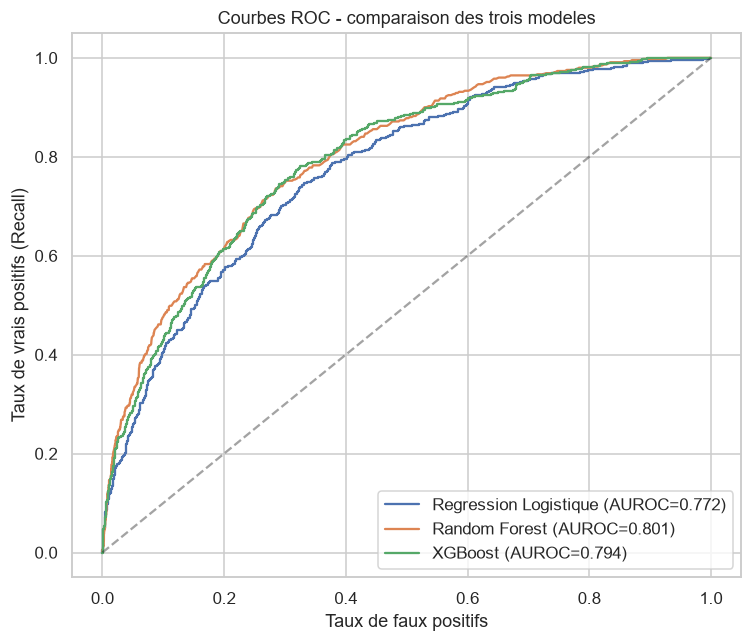
\includegraphics[width=0.62\textwidth]{outputs/courbes_roc.png}
\caption{Courbes \textsc{roc} des trois modèles (échantillon test)}
\label{fig:res-roc}
\end{figure}

\begin{figure}[H]
\centering
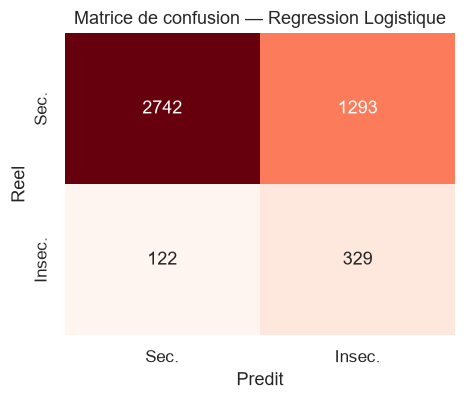
\includegraphics[width=0.45\textwidth]{outputs/matrice_confusion_regression_logistique.png}
\caption{Matrice de confusion de la Régression Logistique (seuil = 0,5)}
\label{fig:res-cm-logit}
\end{figure}

\begin{figure}[H]
\centering
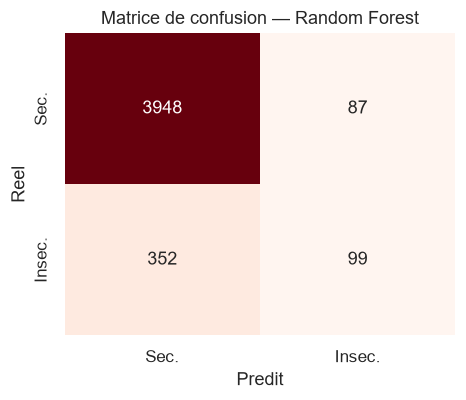
\includegraphics[width=0.45\textwidth]{outputs/matrice_confusion_random_forest.png}
\caption{Matrice de confusion du Random Forest (seuil = 0,5)}
\label{fig:res-cm-rf}
\end{figure}

\begin{figure}[H]
\centering
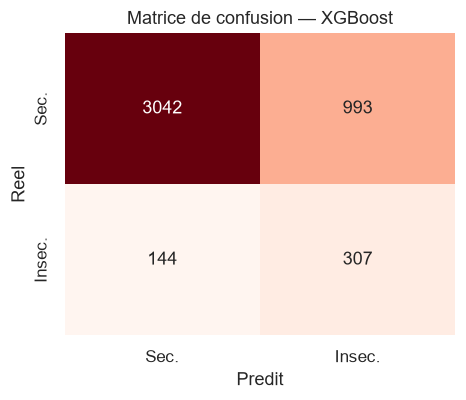
\includegraphics[width=0.45\textwidth]{outputs/matrice_confusion_xgboost.png}
\caption{Matrice de confusion du XGBoost (seuil = 0,5)}
\label{fig:res-cm-xgb}
\end{figure}

\subsubsection{Qualité d'ajustement globale : pseudo-$R^2$ des trois modèles}
\label{sssec:res-pseudor2-comp}

Les trois pseudo-$R^2$ introduits pour le Logit
(Section~\ref{sssec:res-pseudor2}) sont étendus aux deux modèles d'apprentissage
pour comparer la qualité d'ajustement globale des trois approches
(Table~\ref{tab:res-pseudor2}). Une précaution s'impose toutefois : le
\emph{class weighting} \textbf{décalibre volontairement} les probabilités
prédites (il optimise la discrimination, non la vraisemblance), de sorte qu'un
calcul direct sur les probabilités brutes des modèles d'ensemble produirait des
pseudo-$R^2$ négatifs, dénués de sens. Les valeurs inter-modèles sont donc
calculées sur des \textbf{probabilités recalibrées} (régression isotonique
ajustée sur une moitié de l'échantillon test, pseudo-$R^2$ évalué sur l'autre
moitié, sous-ensembles disjoints) ; la valeur classique \emph{in-sample} du
Logit (éq.~14) est rappelée en dernière ligne à titre de référence.

\begin{table}[H]
\centering
\caption{Pseudo-$R^2$ de qualité d'ajustement globale des trois modèles
(probabilités recalibrées sur l'échantillon test, sauf dernière ligne)}
\label{tab:res-pseudor2}
\begin{tabular}{lrrr}
\toprule
\textbf{Modèle} & \textbf{McFadden} & \textbf{Cox-Snell} & \textbf{Nagelkerke} \\
\midrule
Régression Logistique (test recalibré) & 0,147 & 0,091 & 0,191 \\
Random Forest (test recalibré)         & 0,181 & 0,111 & 0,232 \\
XGBoost (test recalibré)               & 0,174 & 0,107 & 0,224 \\
\midrule
Régression Logistique (\emph{in-sample}, éq.~14) & 0,171 & 0,103 & 0,219 \\
\bottomrule
\end{tabular}
\end{table}

Sur des probabilités remises sur un pied de comparabilité, les trois modèles
présentent une qualité d'ajustement globale du même ordre, le
\textbf{Random Forest} (McFadden~=~0,181) et le \textbf{XGBoost}
(0,174) devançant légèrement la régression logistique (0,147). L'ensemble des
pseudo-$R^2$ de McFadden se situe au voisinage du seuil de 0,2 usuellement
associé à un très bon ajustement pour cet indicateur, ce qui conforte, sous un
angle complémentaire à l'\textsc{auroc}, la pertinence des trois modèles et le
léger avantage des méthodes d'ensemble.

\subsubsection{Gestion du déséquilibre : \emph{class weighting} contre \textsc{smote}}

La comparaison prévue à la Section~4.5.2 conforte le choix du
\emph{class weighting} : à hyperparamètres identiques, le XGBoost entraîné sur
données suréchantillonnées par \textsc{smote} obtient une \textsc{auroc}
légèrement inférieure (0,783 contre 0,794) et surtout un \emph{recall}
effondré au seuil de 0,5 (0,118 contre 0,681), rédhibitoire au regard de
l'objectif de détection des ménages vulnérables. Le \emph{class weighting}
présente en outre l'avantage décisif de préserver l'intégration des poids
d'enquête, impossibles à attacher aux observations synthétiques de
\textsc{smote}.

\subsubsection{Analyse de sensibilité à la définition de la variable dépendante}

La hiérarchie des modèles est robuste à la définition de $Y$
(Section~4.2.4) : pour la définition de référence ($\{3,4\}$, prévalence
10,05\,\%) comme pour la définition élargie ($\{2,3,4\}$, 53,20\,\%),
XGBoost domine le Logit (0,794 contre 0,769 et 0,771 contre 0,749
respectivement). Seule la définition stricte ($\{4\}$, 0,83\,\% soit 124~cas)
inverse ponctuellement la hiérarchie (0,814 contre 0,831), inversion à
interpréter avec prudence compte tenu de l'instabilité d'une estimation fondée
sur si peu de cas positifs.

\subsubsection{Calibration des probabilités prédites}

Bruts, les trois modèles sont mal calibrés au sens du test de Hosmer-Lemeshow
($p < 0{,}001$ pour chacun), phénomène attendu : le \emph{class weighting}
optimise la discrimination au détriment de la justesse des probabilités. La
recalibration isotonique du modèle retenu (XGBoost), réalisée sur une moitié de
l'échantillon test et évaluée sur l'autre moitié, corrige ce défaut : le score
de Brier passe de 0,159 à \textbf{0,077} et le test de Hosmer-Lemeshow devient
non significatif ($p = 0{,}479$), indiquant une calibration adéquate
(Figure~\ref{fig:res-calibration}). Le modèle final — XGBoost recalibré — est
donc apte à produire des probabilités interprétables comme des risques réels,
condition posée par l'hypothèse $H_4$ pour le déploiement opérationnel.

\begin{figure}[H]
\centering
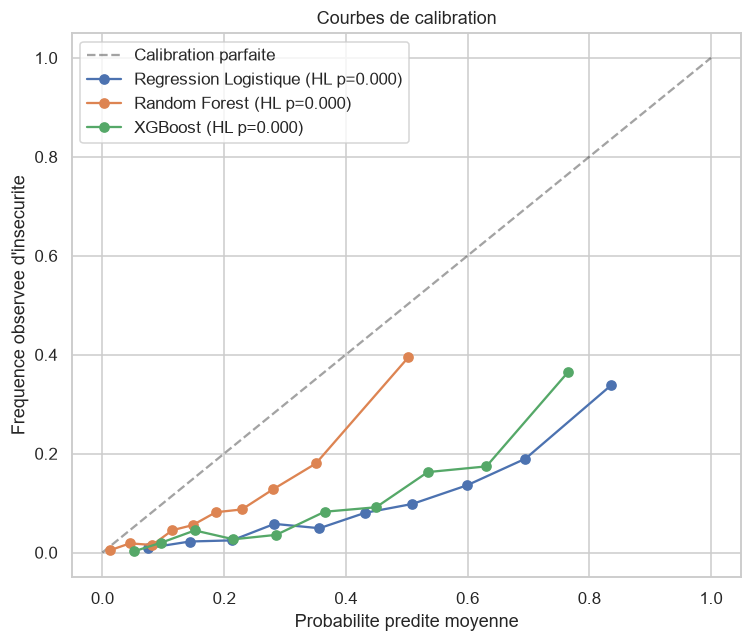
\includegraphics[width=0.62\textwidth]{outputs/calibration.png}
\caption{Courbes de calibration des trois modèles avant recalibration}
\label{fig:res-calibration}
\end{figure}

% ---------------------------------------------------------------------
\subsection{Interprétabilité du modèle retenu : valeurs \textsc{shap}}
\label{ssec:res-shap}

Conformément à la Section~4.7, les valeurs \textsc{shap} ont été calculées pour
les trois modèles (Tree\textsc{shap} pour Random Forest et XGBoost,
Linear\textsc{shap} pour le Logit), sur un échantillon de 1\,200 observations
de l'échantillon test.

\textbf{Importance globale.} Les classements d'importance
(Figure~\ref{fig:res-shap-imp}) convergent avec les déterminants identifiés en
OS1 : les dépenses alimentaires (log), l'accès à l'électricité et le revenu
(log) dominent, suivis de l'indice de qualité du logement et des variables
géographiques (département de l'Atacora). La convergence entre les trois
modèles — pourtant de familles algorithmiques différentes — renforce la
robustesse de ces conclusions.

\textbf{Direction des effets.} Le \emph{summary plot}
(Figure~\ref{fig:res-shap-summary}) confirme le sens des associations : des
dépenses alimentaires faibles, l'absence d'électricité, un revenu faible et un
logement précaire poussent la prédiction vers l'insécurité (valeurs
\textsc{shap} positives), tandis que les niveaux élevés de ces mêmes variables
sont protecteurs.

\textbf{Non-linéarités.} Les \emph{dependence plots} des trois variables les
plus importantes (Figures~\ref{fig:res-shap-dep1}
et~\ref{fig:res-shap-dep2}) révèlent notamment un effet de seuil des dépenses
alimentaires — la contribution au risque devient fortement positive sous un
plancher de dépenses — cohérent avec la non-linéarité détectée par le test de
Box-Tidwell (Section~\ref{ssec:res-bivarie}).

\textbf{Décomposition individuelle.} Les \emph{waterfall plots} de trois
ménages représentatifs illustrent l'usage opérationnel du modèle : pour le
ménage le plus à risque de l'échantillon (probabilité prédite de 0,91 ;
Figure~\ref{fig:res-shap-waterfall}), l'absence de dépenses alimentaires
déclarées (contribution $+0{,}90$ sur l'échelle logit), la résidence dans
l'Atacora ($+0{,}56$), un revenu très faible ($+0{,}16$), l'absence
d'électricité ($+0{,}16$) et l'assistance alimentaire reçue ($+0{,}15$)
constituent l'essentiel du diagnostic. Le
\emph{force plot} interactif du ménage médian, exporté en \textsc{html},
préfigure l'intégration de ces explications individuelles dans l'outil web
(OS4).

\begin{figure}[H]
\centering
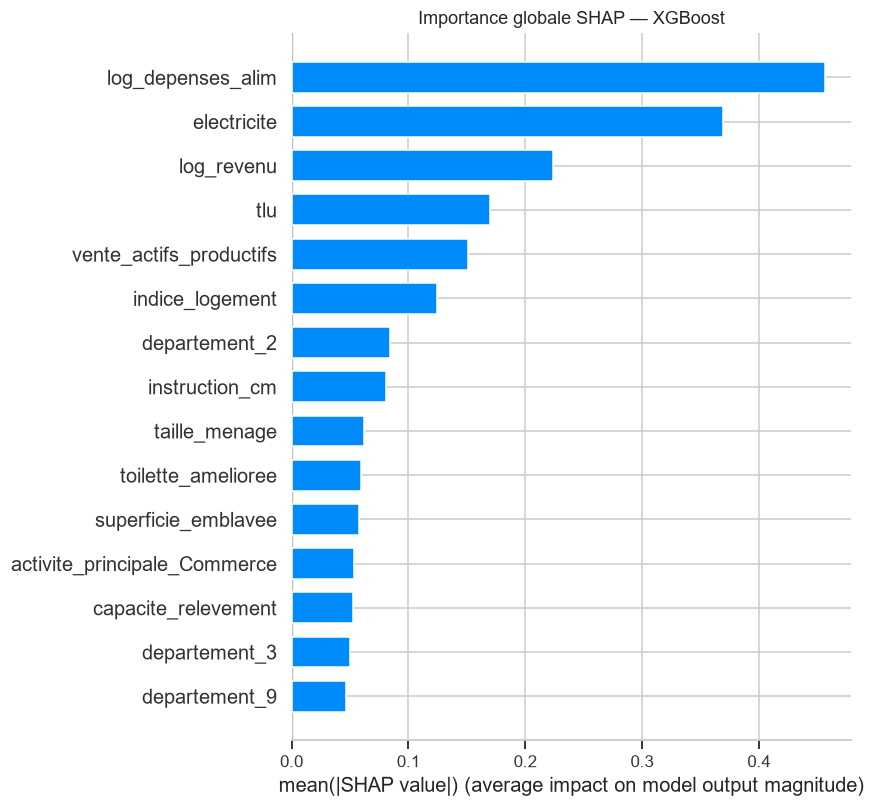
\includegraphics[width=0.72\textwidth]{outputs/shap_importance_xgboost.png}
\caption{Importance globale \textsc{shap} des prédicteurs — XGBoost}
\label{fig:res-shap-imp}
\end{figure}

\begin{figure}[H]
\centering
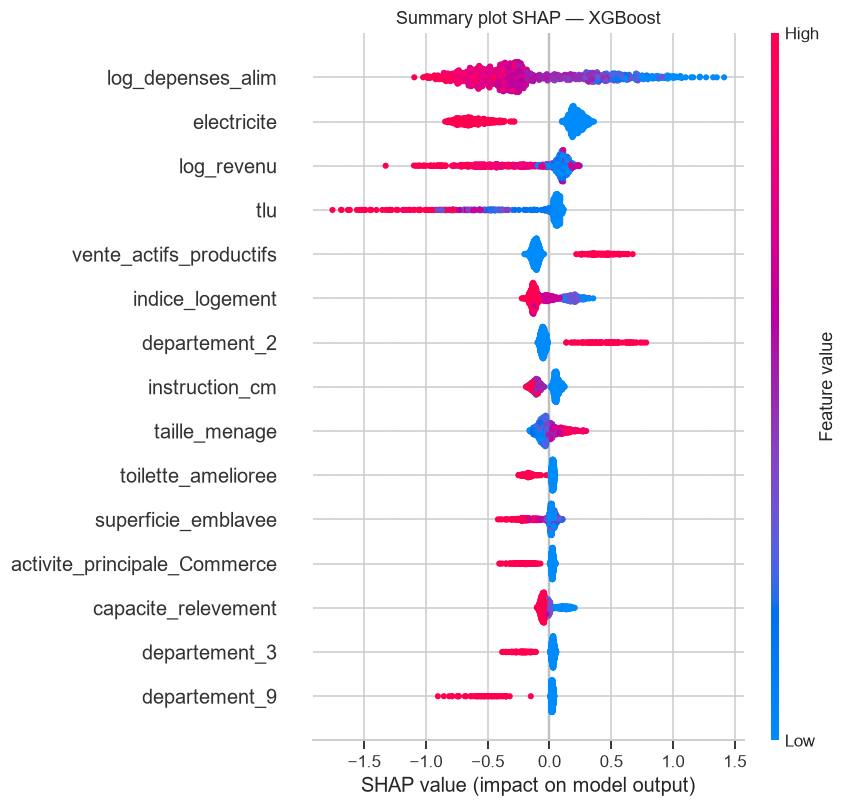
\includegraphics[width=0.72\textwidth]{outputs/shap_summary.png}
\caption{\emph{Summary plot} \textsc{shap} — importance et direction des effets (XGBoost)}
\label{fig:res-shap-summary}
\end{figure}

\begin{figure}[H]
\centering
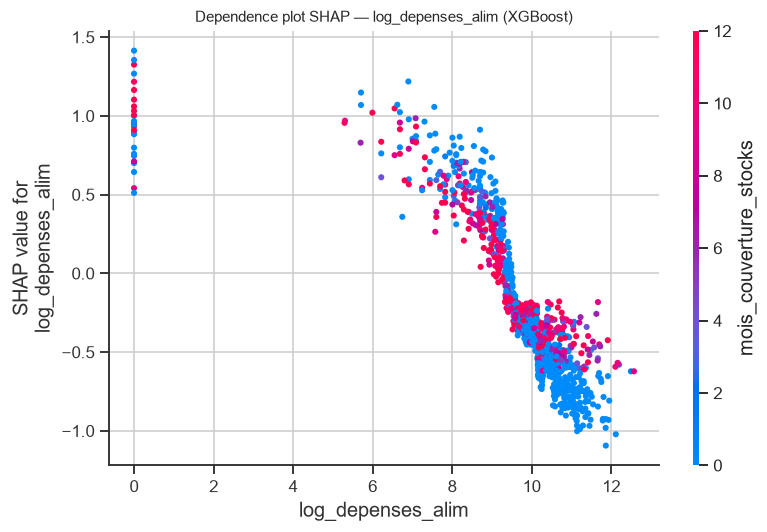
\includegraphics[width=0.6\textwidth]{outputs/shap_dependence_log_depenses_alim.png}
\caption{\emph{Dependence plot} \textsc{shap} des dépenses alimentaires (log)}
\label{fig:res-shap-dep1}
\end{figure}

\begin{figure}[H]
\centering
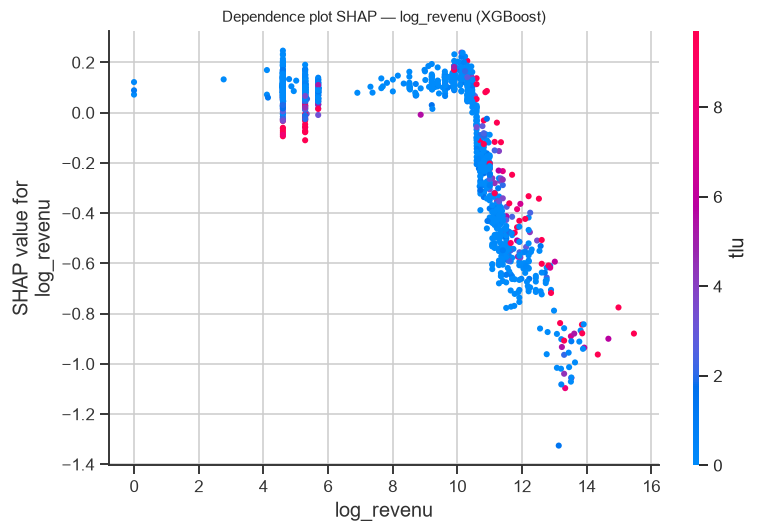
\includegraphics[width=0.6\textwidth]{outputs/shap_dependence_log_revenu.png}
\caption{\emph{Dependence plot} \textsc{shap} du revenu mensuel (log)}
\label{fig:res-shap-dep2}
\end{figure}

\begin{figure}[H]
\centering
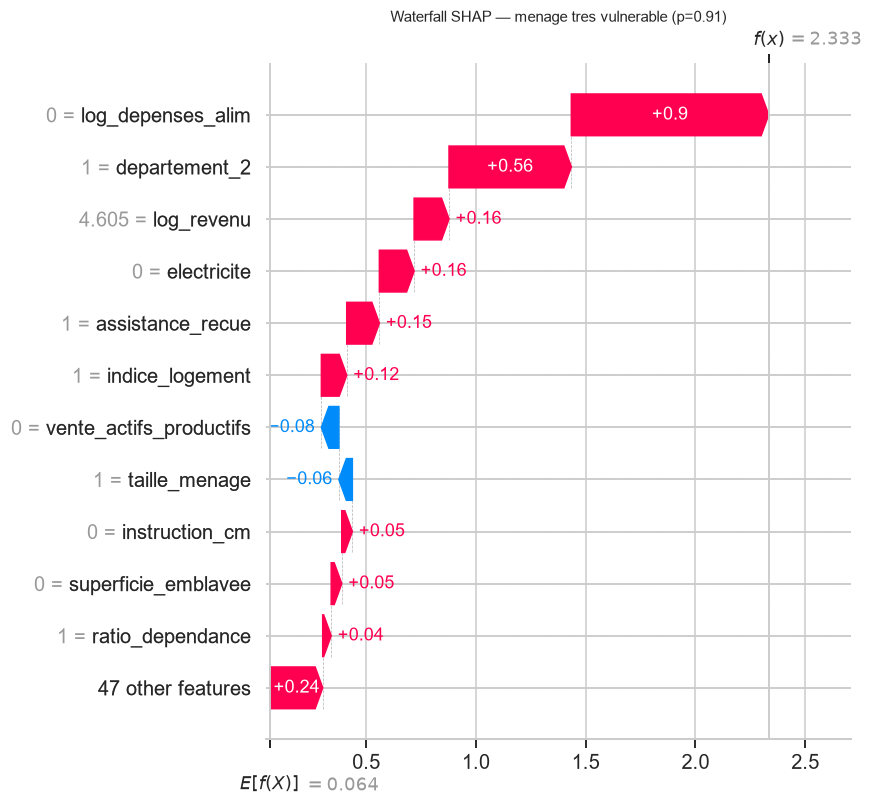
\includegraphics[width=0.72\textwidth]{outputs/shap_waterfall_menage_tres_vulnerable.png}
\caption{\emph{Waterfall plot} \textsc{shap} du ménage le plus vulnérable de l'échantillon
($\hat p = 0{,}91$)}
\label{fig:res-shap-waterfall}
\end{figure}

% ---------------------------------------------------------------------
\subsection{Cartographie communale du risque prédit (OS3)}
\label{ssec:res-os3}

Les probabilités individuelles prédites par le modèle final (XGBoost recalibré)
ont été agrégées par commune avec pondération par les poids d'enquête, puis
jointes au fond de carte des 77~communes (geoBoundaries \textsc{adm}2), avec un
appariement exhaustif (77/77).

\textbf{Autocorrélation spatiale.} L'indice de Moran calculé sur les risques
communaux moyens (matrice de contiguïté de type Queen, standardisée en ligne)
s'établit à $I = 0{,}570$ ($p = 0{,}001$, test par permutations), révélant une
autocorrélation spatiale positive forte et significative : les communes à
risque élevé sont géographiquement groupées. \textbf{L'hypothèse $H_3$ est
confirmée.}

\textbf{Poches de vulnérabilité.} La discrétisation de Jenks en quatre classes
(seuils : 0,08, 0,14 et 0,23) fait apparaître une poche principale de risque
très élevé dans le nord-ouest du pays (département de l'Atacora), et une poche
secondaire dans le centre-sud (Couffo et ouest du Zou)
(Figure~\ref{fig:res-carte}). Les dix communes au risque prédit le plus élevé
sont listées à la Table~\ref{tab:res-communes} : les cinq premières
appartiennent à l'Atacora, Boukoumbé et Toucountouna (39,3\,\% chacune) se
détachant nettement.

\begin{table}[H]
\centering
\caption{Les dix communes au risque prédit d'insécurité alimentaire le plus élevé}
\label{tab:res-communes}
\begin{tabular}{llr}
\toprule
\textbf{Commune} & \textbf{Département} & \textbf{Risque prédit moyen (\%)} \\
\midrule
Boukoumbé    & Atacora & 39,3 \\
Toucountouna & Atacora & 39,3 \\
Tanguiéta    & Atacora & 23,1 \\
Cobly        & Atacora & 22,5 \\
Matéri       & Atacora & 21,5 \\
Agbangnizoun & Zou     & 19,2 \\
Lalo         & Couffo  & 18,9 \\
Natitingou   & Atacora & 18,8 \\
Toviklin     & Couffo  & 17,8 \\
Djakotomey   & Couffo  & 17,4 \\
\bottomrule
\end{tabular}
\end{table}

\begin{figure}[H]
\centering
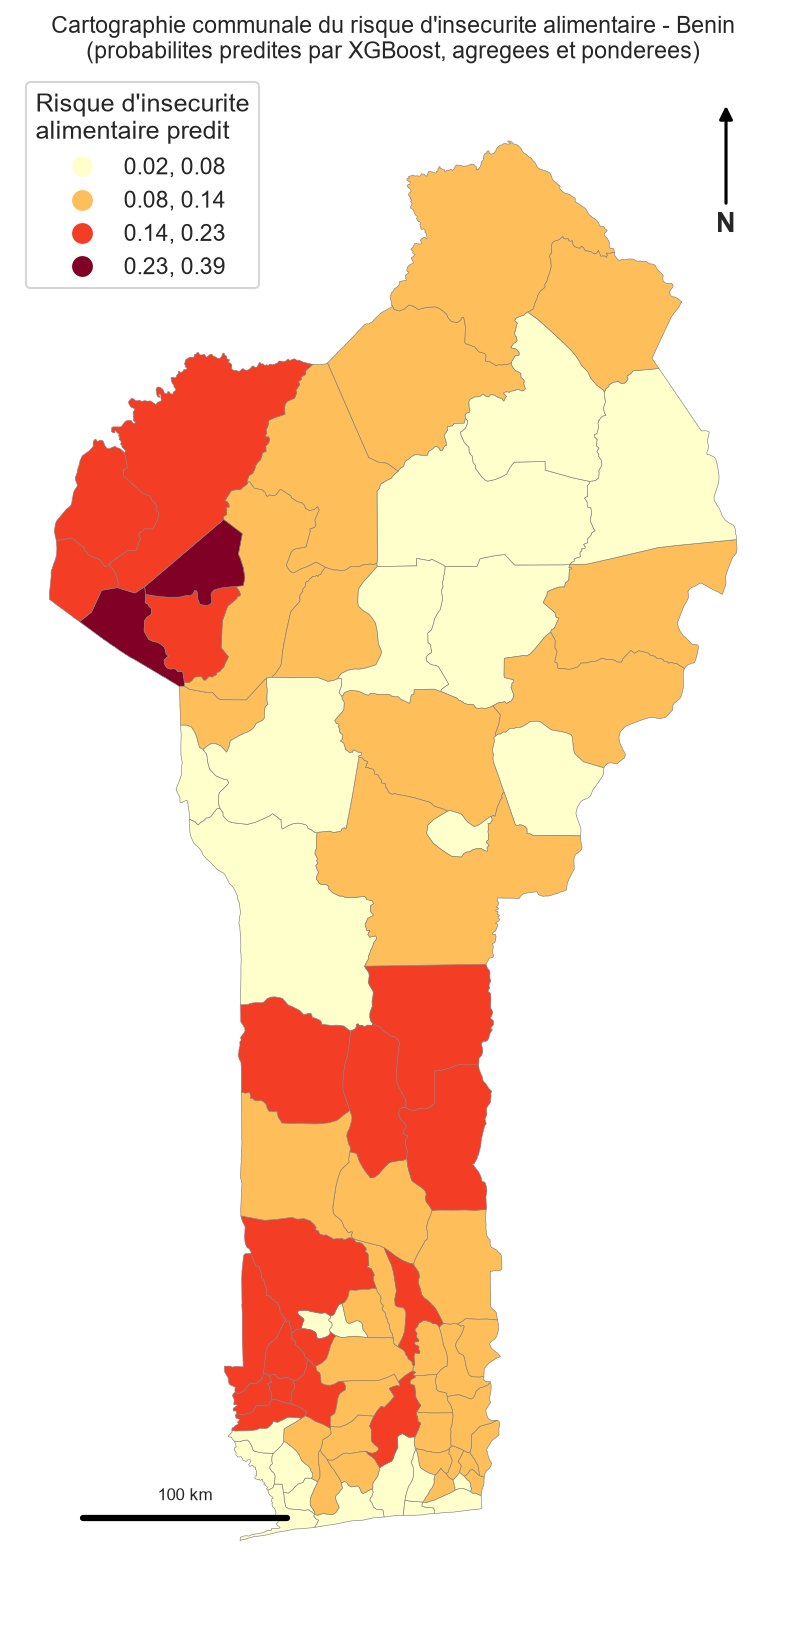
\includegraphics[width=0.8\textwidth]{outputs/carte_risque_communal.png}
\caption{Cartographie communale du risque prédit d'insécurité alimentaire au Bénin
(probabilités du modèle XGBoost, agrégées et pondérées ; discrétisation de Jenks, 4 classes)}
\label{fig:res-carte}
\end{figure}

Ce résultat cartographique converge avec la prévalence départementale observée
(Section~\ref{ssec:res-univarie}) tout en la raffinant à l'échelle communale :
au sein même de l'Atacora, le risque varie du simple au double entre communes,
information directement mobilisable pour le ciblage géographique des
interventions.

% ---------------------------------------------------------------------
\subsection{Produits opérationnels pour l'outil d'aide à la décision (OS4)}
\label{ssec:res-os4}

Le pipeline a produit les artefacts nécessaires au développement de l'outil
d'aide à la décision prévu par l'OS4 :

\begin{itemize}
  \item le \textbf{modèle final sérialisable} (XGBoost recalibré par régression
        isotonique), dont la calibration validée (Brier~=~0,077 ;
        Hosmer-Lemeshow $p = 0{,}479$) autorise des prédictions probabilistes
        fiables sur des ménages hors échantillon au profil similaire à celui de
        l'enquête — condition de l'hypothèse $H_4$ ;
  \item la \textbf{carte interactive} (\texttt{carte\_interactive.html},
        bibliothèque \texttt{folium}) offrant zoom et infobulles communales
        pour la consultation dynamique du risque ;
  \item le \textbf{force plot \textsc{shap} interactif}
        (\texttt{shap\_force\_menage\_median.html}) démontrant la faisabilité
        d'explications individuelles par ménage dans l'application ;
  \item l'\textbf{environnement logiciel figé}
        (\texttt{requirements\_versions.txt}, Section~4.10.1) garantissant la
        reproductibilité du déploiement.
\end{itemize}

Le développement de l'interface applicative elle-même relève des perspectives
et sera discuté au chapitre suivant.

% ---------------------------------------------------------------------
\subsection{Synthèse des résultats au regard des hypothèses de recherche}
\label{ssec:res-hypotheses}

La Table~\ref{tab:res-hypotheses} confronte les résultats obtenus aux quatre
hypothèses formulées au chapitre~2.

\begin{table}[H]
\centering
\caption{Confrontation des résultats aux hypothèses de recherche}
\label{tab:res-hypotheses}
\begin{tabular}{p{0.16\textwidth}p{0.5\textwidth}p{0.24\textwidth}}
\toprule
\textbf{Hypothèse} & \textbf{Résultat empirique} & \textbf{Verdict} \\
\midrule
$H_1$ (OS1) & Éducation (OR = 0,831 ; $p$ = 0,007) et diversification des
revenus (OR = 0,823 ; $p$ = 0,036) significatives ; eau améliorée et résidence
rurale significatives au stade bivarié mais non retenues par le modèle
multivarié (effets absorbés par l'habitat et le département). &
Partiellement validée \\
\addlinespace
$H_2$ (OS2) & AUROC : RF 0,801 $\approx$ XGBoost 0,794 $>$ Logit 0,773 ;
DeLong ML vs Logit significatif ($p \leq 5\times10^{-4}$) ; hiérarchie robuste
aux définitions de $Y$ (hors définition stricte, 124 cas). & Validée \\
\addlinespace
$H_3$ (OS3) & Indice de Moran $I$ = 0,570 ($p$ = 0,001) ; poches concentrées
dans l'Atacora (nord-ouest), secondairement Couffo--Zou. & Validée \\
\addlinespace
$H_4$ (OS4) & Après recalibration isotonique : Brier = 0,077 ;
Hosmer-Lemeshow $p$ = 0,479 ; artefacts opérationnels produits (carte et
explications interactives). & Validée \\
\bottomrule
\end{tabular}
\end{table}

En résumé, l'étude identifie un noyau robuste de déterminants — conditions
économiques du ménage (dépenses, revenu, diversification), capital humain
(instruction, scolarisation), habitat (électricité, qualité du logement) et
ancrage territorial (Atacora) — convergents entre l'approche économétrique
(odds ratios) et l'approche prédictive (valeurs \textsc{shap}) ; elle établit
la supériorité discriminante des algorithmes d'ensemble sur la régression
logistique, sélectionne et calibre un modèle XGBoost opérationnel, et localise
les poches communales de vulnérabilité qui fondent le ciblage géographique des
interventions. Ces résultats sont discutés et mis en perspective au chapitre
suivant.

% ===================== FIN DU CHAPITRE 5 =============================

% =====================================================================

\section{Présentation des résultats}
\label{sec:resultats}

Ce chapitre présente les résultats produits par le pipeline analytique décrit au
chapitre~4, exécuté sous \texttt{Python}~3.11 (\emph{notebook}
\texttt{Pipeline\_Insecurite\_Alimentaire\_Benin.ipynb}, graine aléatoire
\texttt{RANDOM\_STATE = 42}). La présentation suit la progression logique des
objectifs spécifiques : constitution et validation de la variable dépendante
(Section~\ref{ssec:res-echantillon}), analyse descriptive univariée et bivariée
(Sections~\ref{ssec:res-univarie} à~\ref{ssec:res-bivarie}), identification des
déterminants — OS1 (Section~\ref{ssec:res-os1}), comparaison des modèles
prédictifs — OS2 (Section~\ref{ssec:res-os2}), interprétabilité \textsc{shap}
(Section~\ref{ssec:res-shap}), cartographie communale du risque — OS3
(Section~\ref{ssec:res-os3}) et produits opérationnels pour l'outil d'aide à la
décision — OS4 (Section~\ref{ssec:res-os4}). Une synthèse confronte enfin les
résultats aux hypothèses de recherche (Section~\ref{ssec:res-hypotheses}).

% ---------------------------------------------------------------------
\subsection{Constitution de l'échantillon analytique et validation de la variable dépendante}
\label{ssec:res-echantillon}

\subsubsection{Échantillon analytique et prévalence de l'insécurité alimentaire}

La base AGVSAN 2017 compte 14\,952 ménages et 1\,406 variables. La variable
\texttt{Round\_INDICE\_SECAL} est renseignée pour la totalité des ménages :
aucune observation n'a été exclue et l'échantillon analytique est de
$n = 14\,952$. La Table~\ref{tab:res-repartition-y} présente la répartition des
quatre classes \textsc{cari} et les prévalences associées aux trois définitions
de la variable dépendante.

\begin{table}[H]
\centering
\caption{Répartition des classes \textsc{cari} et prévalence de $Y$ selon les trois définitions}
\label{tab:res-repartition-y}
\small\setlength{\tabcolsep}{4pt}
\begin{tabular}{lrr}
\toprule
\textbf{Classe \textsc{cari}} & \textbf{Effectif} & \textbf{\%} \\
\midrule
1 — Sécurité alimentaire          & 6\,998 & 46,80 \\
2 — Sécurité alimentaire limite   & 6\,452 & 43,15 \\
3 — Insécurité modérée            & 1\,378 &  9,22 \\
4 — Insécurité sévère             &    124 &  0,83 \\
\midrule
\textbf{Définition de $Y$}        & \textbf{Prévalence brute} & \textbf{Prévalence pondérée} \\
\midrule
Référence $\{3,4\}$               & 10,05\,\% & 9,66\,\% \\
Stricte $\{4\}$                   &  0,83\,\% & --- \\
Élargie $\{2,3,4\}$               & 53,20\,\% & --- \\
\bottomrule
\end{tabular}
\end{table}

Selon la définition de référence, 1\,502 ménages (10,05\,\% ; 9,66\,\% après
pondération par les poids d'enquête \texttt{weight\_agvsa}) sont en insécurité
alimentaire. Ce fort déséquilibre de classes justifie \emph{a posteriori} la
stratégie de \emph{class weighting} retenue au chapitre~4 (Section~4.5.2). La
prévalence pondérée est nettement différenciée selon le milieu de résidence :
13,03\,\% en milieu rural contre 6,19\,\% en milieu urbain (et 1,52\,\%
seulement à Cotonou), premier indice de la dimension territoriale du phénomène.

\subsubsection{Validation croisée de la classification officielle}

Conformément à la Section~4.2.4, le \textsc{sca} a été reconstruit de manière
indépendante à partir des 18~items bruts de consommation alimentaire
(moyenne~=~49,8 ; médiane~=~50,5 ; étendue 0--112). Sa répartition selon les
seuils standard du \textsc{pam} est : pauvre ($<28$) 1\,435 ménages (9,6\,\%),
limite (28--42) 3\,387 (22,7\,\%), acceptable ($>42$) 10\,130 (67,7\,\%). La
concordance entre le \textsc{sca} reconstruit dichotomisé
($\textsc{sca} \leq 42$) et la classification officielle dichotomisée s'établit
à \textbf{76,1\,\% d'accord global} avec un \textbf{Kappa de Cohen de 0,333},
et la corrélation ordinale entre le \textsc{sca} et la classe \textsc{cari} est
négative et hautement significative (Spearman $\rho = -0{,}371$ ;
$p < 0{,}001$), dans le sens attendu (un \textsc{sca} plus faible correspond à
une classe plus sévère). Cette concordance modérée est conforme à la
littérature : la classification \textsc{cari} officielle combine le \textsc{sca}
avec le \textsc{rcsi} et la part des dépenses alimentaires, de sorte qu'une
concordance parfaite avec le seul \textsc{sca} n'est pas attendue.

La validation par l'indice de stratégies de survie confirme la cohérence de la
variable dépendante : le \textsc{rcsi} moyen est de 18,96 chez les ménages en
insécurité contre 10,79 chez les ménages en sécurité (test unilatéral de
Mann-Whitney, $p = 2{,}2 \times 10^{-66}$).

\paragraph{Limite relative au \textsc{hfias}.} Le score \textsc{hfias} prévu
comme second indicateur de validation (Section~4.2.5) s'est révélé
\textbf{indisponible} dans la base ménage transmise (la colonne \texttt{Q\_9\_05}
du fichier correspond à un autre champ du questionnaire). La validation croisée
repose donc sur le seul \textsc{rcsi}, limite qui sera discutée au chapitre
suivant.

% ---------------------------------------------------------------------
\subsection{Analyse univariée des variables focales}
\label{ssec:res-univarie}

\subsubsection{Situation alimentaire des ménages}

Au niveau national, 89,95\,\% des ménages sont en sécurité alimentaire et
10,05\,\% en insécurité (90,34\,\% et 9,66\,\% après pondération ;
Figure~\ref{fig:res-y-national}). La stratification par département
(Figure~\ref{fig:res-y-departement}) révèle de fortes disparités : la
prévalence brute varie de 1,52\,\% dans le Littoral à \textbf{22,80\,\% dans
l'Atacora}, suivi du Couffo (16,40\,\%), des Collines (15,74\,\%) et du Zou
(11,63\,\%), tous au-dessus de la moyenne nationale. Cette hétérogénéité
géographique, déjà visible au stade descriptif, annonce les résultats de la
cartographie prédictive (Section~\ref{ssec:res-os3}).

\begin{figure}[H]
\centering
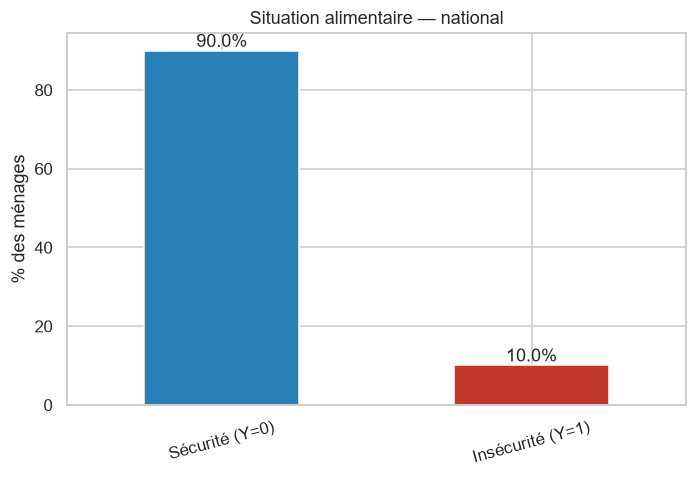
\includegraphics[width=0.62\textwidth]{outputs/univarie_Y_national.png}
\caption{Répartition nationale des ménages selon la situation alimentaire ($Y$)}
\label{fig:res-y-national}
\end{figure}

\begin{figure}[H]
\centering
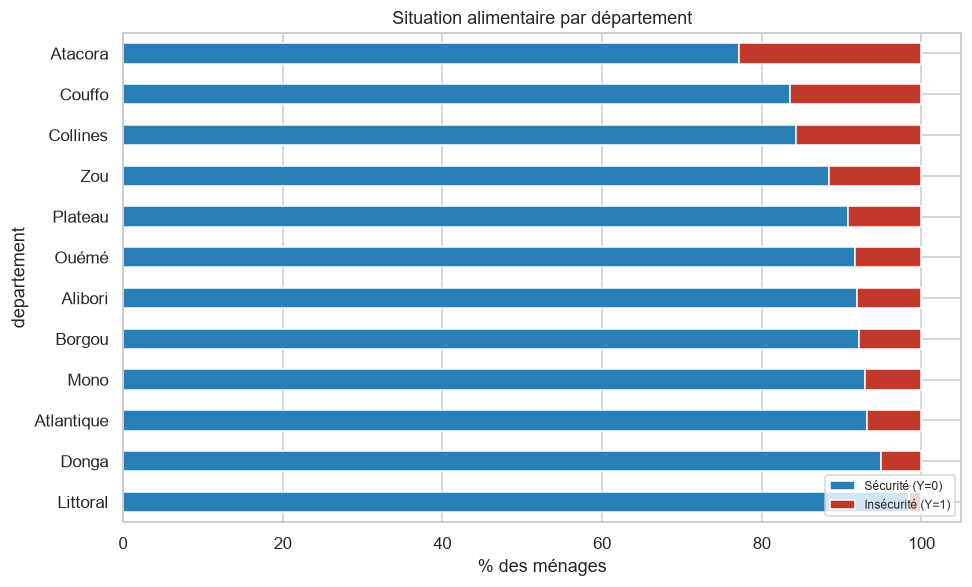
\includegraphics[width=0.85\textwidth]{outputs/univarie_Y_departement.png}
\caption{Situation alimentaire des ménages par département (barres empilées, \% en ligne)}
\label{fig:res-y-departement}
\end{figure}

\subsubsection{Taille des ménages}

La taille moyenne des ménages est de 6,83 personnes (médiane~=~6 ;
écart-type~=~4,57 ; CV~=~66,9\,\%), avec une distribution asymétrique à droite
(skewness~=~2,88) s'étirant jusqu'à 86 personnes
(Figure~\ref{fig:res-taille-hist}). Les ménages ruraux sont en moyenne plus
grands que les ménages urbains (7,2 contre 6,4 personnes ;
Figure~\ref{fig:res-taille-box}), les percentiles extrêmes confirmant cet écart
($P_{90}$ de 13 en milieu rural contre 11 en milieu urbain).

\begin{figure}[H]
\centering
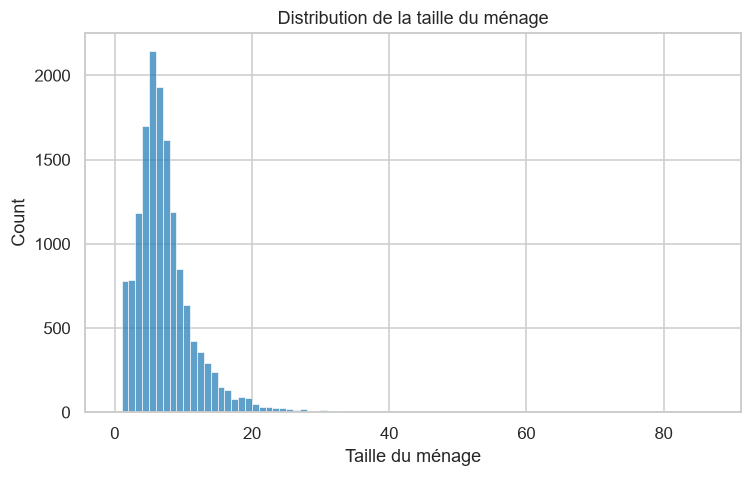
\includegraphics[width=0.62\textwidth]{outputs/univarie_taille_hist.png}
\caption{Distribution de la taille des ménages}
\label{fig:res-taille-hist}
\end{figure}

\begin{figure}[H]
\centering
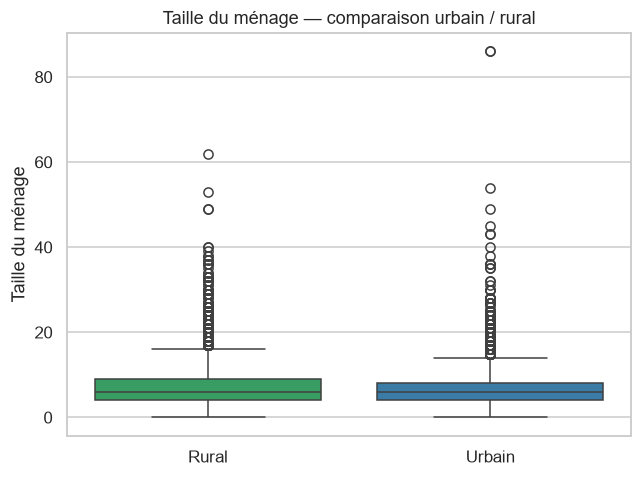
\includegraphics[width=0.55\textwidth]{outputs/univarie_taille_boxplot.png}
\caption{Taille des ménages : comparaison urbain / rural (boîtes à moustaches)}
\label{fig:res-taille-box}
\end{figure}

\subsubsection{Revenu mensuel}

Le revenu mensuel déclaré présente l'asymétrie extrême caractéristique des
données de revenu : moyenne de 68\,105 \textsc{fcfa} pour une médiane de
15\,000 \textsc{fcfa}, écart-type de 217\,941 \textsc{fcfa}
(CV~=~320\,\%), skewness de 11,06 et kurtosis de 181,8
(Figure~\ref{fig:res-revenu-brut}). La transformation logarithmique
$\ln(\text{revenu}+1)$ retenue pour la modélisation (Section~4.3.3) ramène la
skewness à $-0{,}06$, soit une distribution quasi symétrique
(Figure~\ref{fig:res-revenu-log}), ce qui valide empiriquement ce choix
méthodologique.

\begin{figure}[H]
\centering
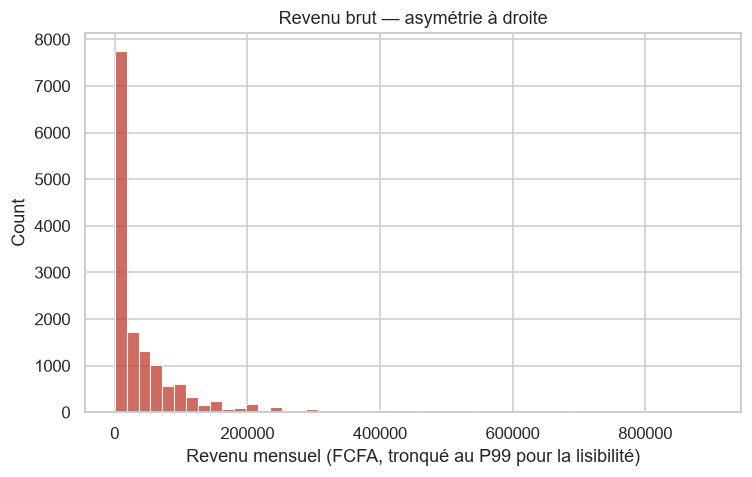
\includegraphics[width=0.62\textwidth]{outputs/univarie_revenu_brut.png}
\caption{Distribution du revenu mensuel brut (\textsc{fcfa}, tronqué au $P_{99}$)}
\label{fig:res-revenu-brut}
\end{figure}

\begin{figure}[H]
\centering
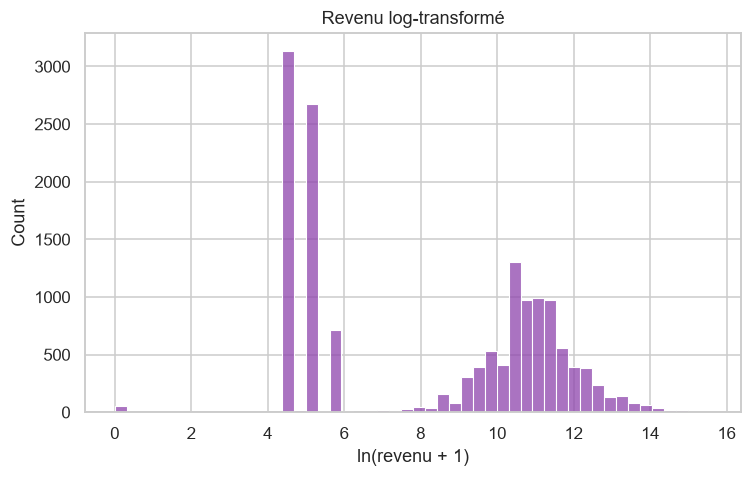
\includegraphics[width=0.62\textwidth]{outputs/univarie_revenu_log.png}
\caption{Distribution du revenu log-transformé $\ln(\text{revenu}+1)$}
\label{fig:res-revenu-log}
\end{figure}

\subsubsection{Âge du chef de ménage}

L'âge moyen du chef de ménage est de 47,1 ans (médiane~=~45 ;
écart-type~=~15,0 ; étendue 16--100 ans), avec une asymétrie modérée
(skewness~=~0,70 ; Figure~\ref{fig:res-age}). La répartition par tranches
usuelles est la suivante : moins de 30~ans, 8,94\,\% ; 30--44~ans, 37,22\,\% ;
45--59~ans, 32,30\,\% ; 60~ans et plus, 21,54\,\%.

\begin{figure}[H]
\centering
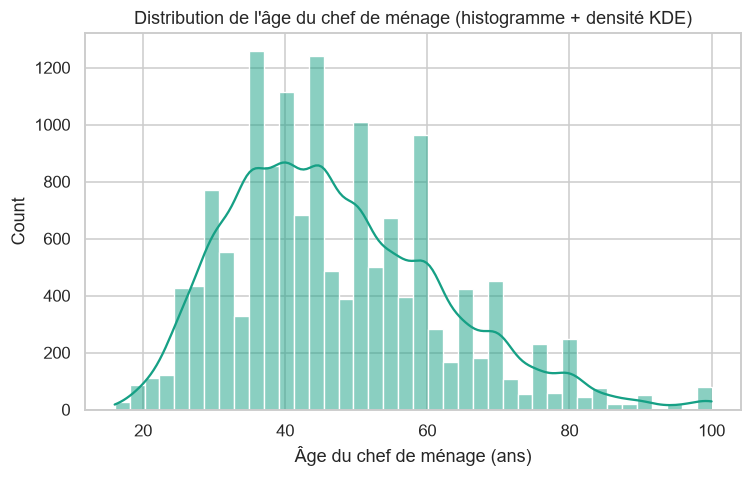
\includegraphics[width=0.62\textwidth]{outputs/univarie_age.png}
\caption{Distribution de l'âge du chef de ménage (histogramme et densité à noyau)}
\label{fig:res-age}
\end{figure}

\subsubsection{Niveau d'instruction du chef de ménage}

Plus de la moitié des chefs de ménage (51,22\,\%) n'ont aucune instruction
formelle ; viennent ensuite le primaire (22,59\,\%), le secondaire (17,04\,\%),
le supérieur (4,47\,\%), l'alphabétisation (3,36\,\%), l'école coranique
(1,17\,\%) et le cursus arabe (0,06\,\%) (Figure~\ref{fig:res-instruction}).
Après recodage en trois niveaux (Table~5 du chapitre~4), la répartition est :
\emph{Aucun/informel} 55,89\,\%, \emph{Primaire} 22,59\,\%,
\emph{Secondaire et plus} 21,52\,\%.

\begin{figure}[H]
\centering
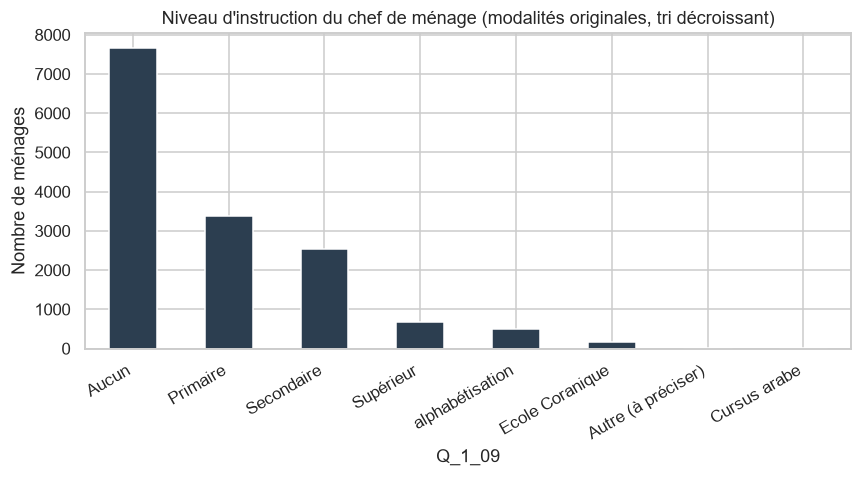
\includegraphics[width=0.72\textwidth]{outputs/univarie_instruction.png}
\caption{Niveau d'instruction du chef de ménage (modalités originales, tri décroissant)}
\label{fig:res-instruction}
\end{figure}

\subsubsection{Accès au crédit}

Un peu plus du quart des ménages (25,79\,\% ; 26,26\,\% pondéré) a contracté un
emprunt au cours des douze derniers mois. L'accès au crédit est légèrement plus
fréquent en milieu rural (27,31\,\%) qu'en milieu urbain (23,99\,\%)
(Figure~\ref{fig:res-credit-univ}).

\begin{figure}[H]
\centering
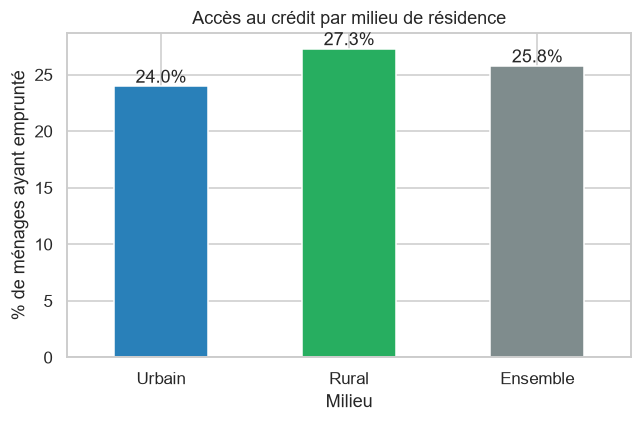
\includegraphics[width=0.55\textwidth]{outputs/univarie_credit.png}
\caption{Proportion de ménages ayant accès au crédit, par milieu de résidence}
\label{fig:res-credit-univ}
\end{figure}

% ---------------------------------------------------------------------
\subsection{Tests de normalité des variables continues}
\label{ssec:res-normalite}

La Table~\ref{tab:res-normalite} rapporte les tests de normalité prévus à la
Section~4.4.3. Pour les quatre variables continues focales, l'hypothèse de
normalité est rejetée par le test de Kolmogorov-Smirnov comme par celui de
Shapiro-Wilk ($p < 0{,}001$ dans tous les cas), conclusion corroborée par les
coefficients de forme et par les QQ-plots
(Figures~\ref{fig:res-qq-taille} et~\ref{fig:res-qq-age}). Conformément à la
règle de décision du chapitre~4 — et en tenant compte de la puissance très
élevée de ces tests avec $n \approx 15\,000$ — l'analyse bivariée recourt
systématiquement au test non paramétrique de Mann-Whitney pour les variables
continues.

\begin{table}[H]
\centering
\caption{Tests de normalité des variables continues focales ($n = 14\,952$)}
\label{tab:res-normalite}
\small\setlength{\tabcolsep}{4pt}
\begin{tabular}{lrrrrrl}
\toprule
\textbf{Variable} & \textbf{KS $D_n$} & \textbf{KS $p$} & \textbf{Shapiro $W$} & \textbf{Skew.} & \textbf{Kurt.} & \textbf{Conclusion} \\
\midrule
Taille du ménage        & 0,164 & $<0{,}001$ & 0,813 &  2,88 & 22,24  & Normalité rejetée \\
Revenu brut (\textsc{fcfa}) & 0,377 & $<0{,}001$ & 0,267 & 11,06 & 181,85 & Normalité rejetée \\
$\ln(\text{revenu}+1)$  & 0,239 & $<0{,}001$ & 0,848 & $-0{,}06$ & $-1{,}54$ & Normalité rejetée \\
Âge du chef de ménage   & 0,092 & $<0{,}001$ & 0,969 &  0,70 & 0,33   & Normalité rejetée \\
\bottomrule
\end{tabular}
\end{table}

\begin{figure}[H]
\centering
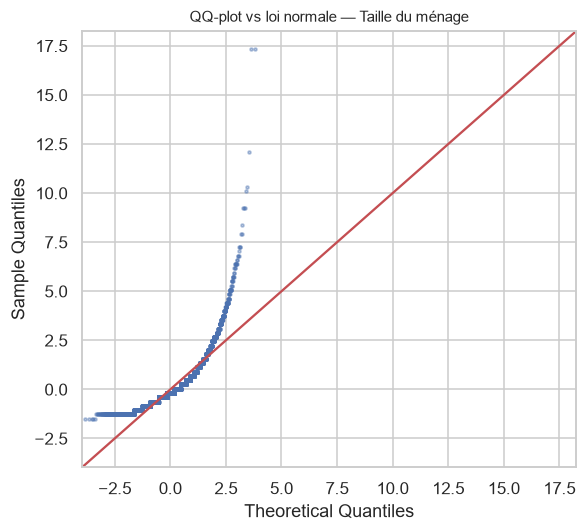
\includegraphics[width=0.48\textwidth]{outputs/normalite_qq_taille.png}
\caption{QQ-plot de la taille du ménage contre la loi normale standard}
\label{fig:res-qq-taille}
\end{figure}

\begin{figure}[H]
\centering
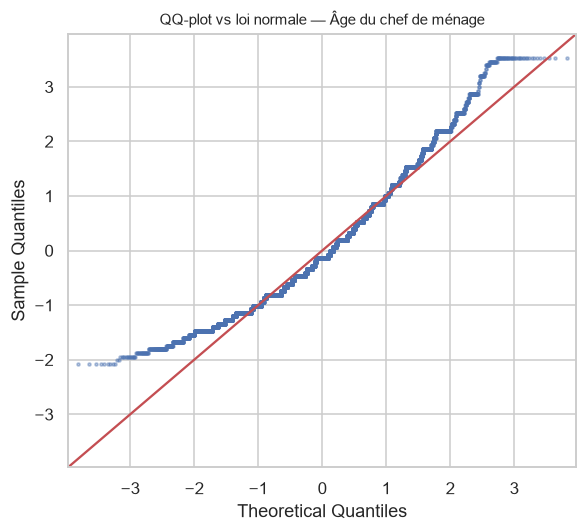
\includegraphics[width=0.48\textwidth]{outputs/normalite_qq_age.png}
\caption{QQ-plot de l'âge du chef de ménage contre la loi normale standard}
\label{fig:res-qq-age}
\end{figure}

% ---------------------------------------------------------------------
\subsection{Analyse bivariée et tests pré-estimation}
\label{ssec:res-bivarie}

\subsubsection{Variables focales croisées avec la situation alimentaire}

La Table~\ref{tab:res-bivarie-focales} synthétise les tests bivariés conduits
selon le canevas de la Section~4.4.4 (le test de Levene ayant orienté, avec le
rejet de la normalité, vers le test de Mann-Whitney pour les continues).

\begin{table}[H]
\centering
\caption{Analyse bivariée des variables focales $\times$ situation alimentaire ($Y$)}
\label{tab:res-bivarie-focales}
\small\setlength{\tabcolsep}{3.5pt}
\begin{tabular}{lllrl}
\toprule
\textbf{Variable} & \textbf{Test} & \textbf{Statistique} & \textbf{$p$-valeur} & \textbf{Conclusion} \\
\midrule
Taille du ménage        & Mann-Whitney & $U = 9\,667\,365{,}5$  & 0,006                 & Significatif \\
$\ln(\text{revenu}+1)$  & Mann-Whitney & $U = 8\,119\,697{,}0$  & $2{,}7\times10^{-36}$ & Significatif \\
Âge du chef de ménage   & Mann-Whitney & $U = 10\,613\,702{,}0$ & 0,001                 & Significatif \\
Niveau d'instruction    & $\chi^2$ (ddl = 2) & $\chi^2 = 226{,}06$ ; $V = 0{,}123$ & $8{,}2\times10^{-50}$ & Significatif \\
Accès au crédit         & $\chi^2$ (2$\times$2) & $\chi^2 = 0{,}013$ ; OR = 0,991 & 0,908 & \textbf{Non significatif} \\
\bottomrule
\end{tabular}
\end{table}

Quatre enseignements ressortent de cette analyse.

\textbf{(i) Le revenu est le facteur focal le plus discriminant.} Le revenu
log-transformé des ménages en insécurité est très inférieur à celui des ménages
en sécurité (médianes de 5,70 contre 9,63 sur l'échelle log, soit environ 297
contre 15\,198 \textsc{fcfa} sur l'échelle brute ;
$p = 2{,}7\times10^{-36}$ ; Figure~\ref{fig:res-box-revenu}), résultat cohérent
avec l'approche des pièges à pauvreté discutée au chapitre~3.

\textbf{(ii) Le gradient d'instruction est net et monotone.} La prévalence de
l'insécurité décroît régulièrement avec le niveau d'instruction du chef de
ménage : 13,17\,\% (\emph{Aucun/informel}), 7,73\,\% (\emph{Primaire}),
4,35\,\% (\emph{Secondaire et plus}) ($\chi^2(2) = 226{,}06$ ;
$V$ de Cramér~=~0,123 ; Figure~\ref{fig:res-biv-instruction}), conformément à
la littérature.

\textbf{(iii) Deux résultats vont à rebours de l'intuition.} D'une part, les
ménages en insécurité sont en moyenne légèrement \emph{plus petits} que les
ménages en sécurité (6,54 contre 6,87 personnes ; $p = 0{,}006$ ;
Figure~\ref{fig:res-box-taille}). D'autre part, la relation entre l'âge du chef
de ménage et l'insécurité est en U : la prévalence est plus élevée aux deux
extrémités de la distribution (11,23\,\% avant 30~ans et 12,79\,\% à 60~ans et
plus, contre 8,97\,\% et 9,13\,\% pour les tranches intermédiaires), les
moyennes différant significativement (48,69 contre 46,93 ans ; $p = 0{,}001$ ;
Figure~\ref{fig:res-box-age}).

\textbf{(iv) L'accès au crédit n'est pas associé au statut alimentaire.} La
prévalence de l'insécurité est quasi identique chez les ménages emprunteurs
(9,98\,\%) et non emprunteurs (10,07\,\%), et l'odds ratio brut est nul au sens
statistique (OR~=~0,991 ; IC à 95\,\% $[0{,}877\,;\,1{,}120]$ ; $p = 0{,}908$ ;
Figure~\ref{fig:res-biv-credit}). Ce résultat nul, contraire à l'hypothèse
d'un rôle protecteur du crédit, sera repris dans la discussion.

\begin{figure}[H]
\centering
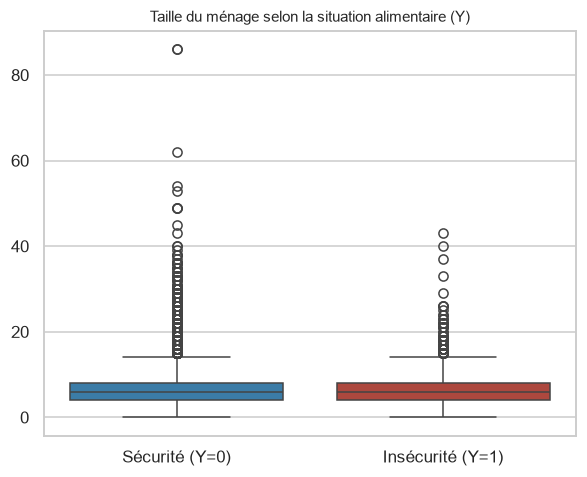
\includegraphics[width=0.5\textwidth]{outputs/bivarie_boxplot_taille.png}
\caption{Taille du ménage selon la situation alimentaire}
\label{fig:res-box-taille}
\end{figure}

\begin{figure}[H]
\centering
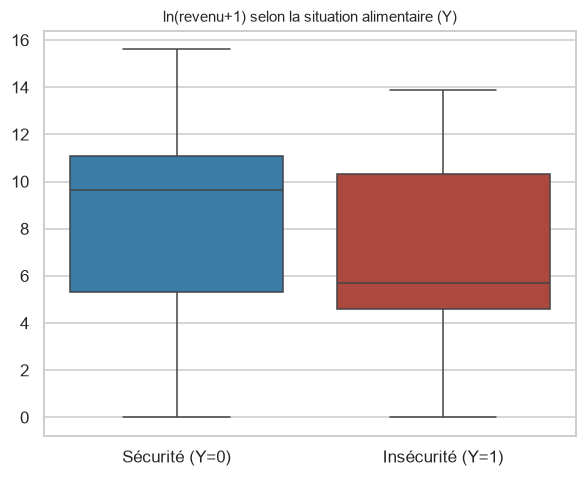
\includegraphics[width=0.5\textwidth]{outputs/bivarie_boxplot_revenu.png}
\caption{Revenu log-transformé selon la situation alimentaire}
\label{fig:res-box-revenu}
\end{figure}

\begin{figure}[H]
\centering
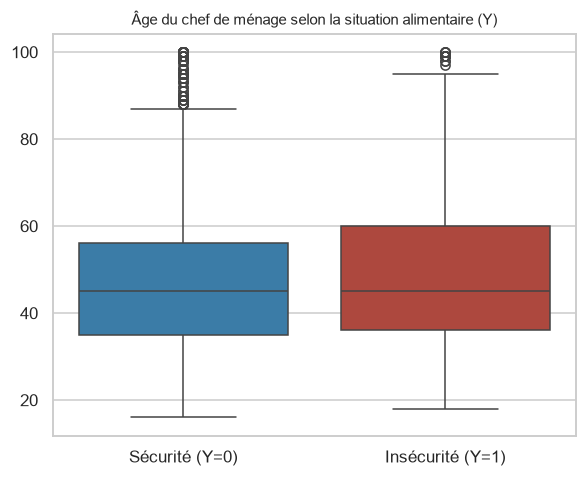
\includegraphics[width=0.5\textwidth]{outputs/bivarie_boxplot_age.png}
\caption{Âge du chef de ménage selon la situation alimentaire}
\label{fig:res-box-age}
\end{figure}

\begin{figure}[H]
\centering
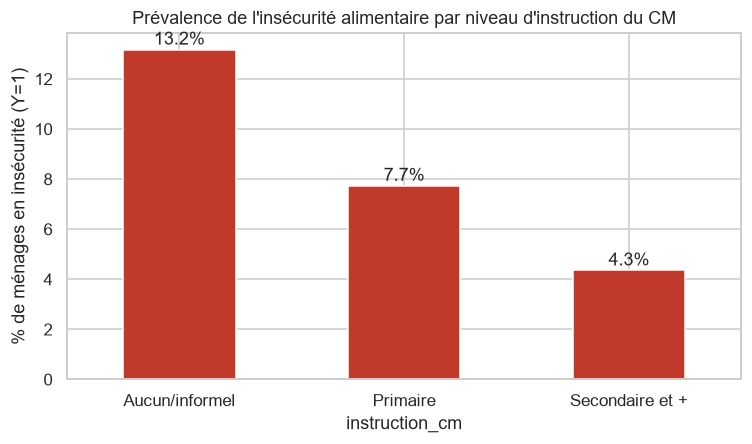
\includegraphics[width=0.62\textwidth]{outputs/bivarie_instruction.png}
\caption{Prévalence de l'insécurité alimentaire selon le niveau d'instruction du chef de ménage}
\label{fig:res-biv-instruction}
\end{figure}

\begin{figure}[H]
\centering
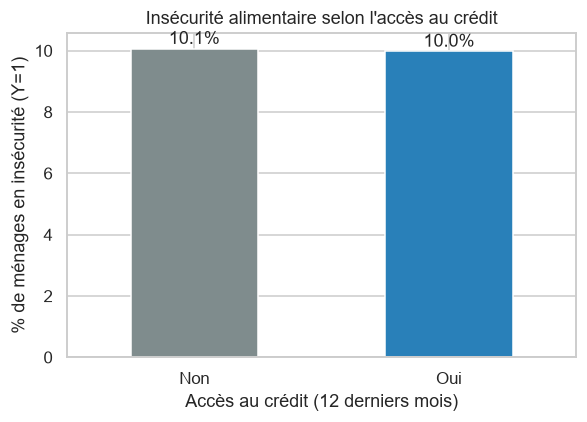
\includegraphics[width=0.5\textwidth]{outputs/bivarie_credit.png}
\caption{Prévalence de l'insécurité alimentaire selon l'accès au crédit}
\label{fig:res-biv-credit}
\end{figure}

\subsubsection{Tests bivariés étendus et correction pour comparaisons multiples}

L'analyse a été étendue à l'ensemble des variables indépendantes retenues
(Table~10 du chapitre~4), soit 22~tests, avec correction de Benjamini-Hochberg
(contrôle du \textsc{fdr}). Après correction, \textbf{20 des 22 variables
demeurent significativement associées} au statut alimentaire au seuil de
5\,\% ; seules la possession de bétail (\textsc{tlu}, $p_{aj} = 0{,}709$) et
l'accès au crédit ($p_{aj} = 0{,}908$) ne le sont pas. Les associations les
plus fortes concernent, par ordre de $p$-valeur ajustée croissante : les
dépenses alimentaires (log), l'accès à l'électricité ($V = 0{,}169$), le
département ($V = 0{,}179$), l'indice de qualité du logement, le niveau
d'instruction, le milieu de résidence ($V = 0{,}115$) et le revenu (log). La
nouvelle variable « mois de couverture des stocks » est également associée au
statut alimentaire ($p_{aj} < 0{,}001$), les ménages en insécurité déclarant
paradoxalement une couverture médiane plus longue (2~mois contre 0), reflet de
leur profil plus agricole.

\subsubsection{Multicolinéarité et linéarité dans le logit}

Aucune colinéarité problématique n'est détectée parmi les prédicteurs continus :
tous les \textsc{vif} sont inférieurs à 2 (maximum : diversification des
revenus, \textsc{vif} = 1,82). Pour les variables polytomiques, le \textsc{gvif}
de Fox et Monette conduit à la même conclusion
(Table~\ref{tab:res-gvif}) : la valeur normalisée maximale
$\text{GVIF}^{1/(2\,\text{ddl})} = 1{,}78$ (type de choc) reste sous le seuil
de $\sqrt{5} \approx 2{,}24$. L'ensemble des prédicteurs peut donc être
conservé dans le modèle logistique.

\begin{table}[H]
\centering
\caption{GVIF des variables polytomiques (Fox et Monette, 1992)}
\label{tab:res-gvif}
\begin{tabular}{lrrr}
\toprule
\textbf{Variable} & \textbf{ddl} & \textbf{GVIF} & \textbf{GVIF$^{1/(2\,\text{ddl})}$} \\
\midrule
Statut matrimonial    &  5 &   2,155 & 1,080 \\
Département           & 11 &   6,231 & 1,087 \\
Activité principale   &  5 &   5,163 & 1,178 \\
Type de choc          &  4 & 102,411 & 1,784 \\
\bottomrule
\end{tabular}
\end{table}

Le test de Box-Tidwell (Section~4.5.3) conclut à une linéarité acceptable dans
le logit pour l'âge ($p = 0{,}61$), la taille du ménage ($p = 0{,}21$) et le
ratio de dépendance ($p = 0{,}11$) ; seules les dépenses alimentaires (log)
présentent une non-linéarité significative ($p = 3{,}9\times10^{-18}$),
qu'avec $n \approx 15\,000$ il convient de relativiser et que les modèles
d'arbres (Random Forest, XGBoost), non paramétriques, capturent par
construction.

\subsubsection{Robustesse au plan de sondage : analyse pondérée design-based}
\label{sssec:res-ponderee}

Conformément à la Section~4.5.1, les statistiques descriptives et les tests
bivariés ont été recalculés en tenant compte du plan de sondage complexe
(poids \texttt{weight\_agvsa}, grappes en unités primaires, strates
reconstruites «~département~$\times$~milieu~») au moyen du package
\texttt{samplics} (linéarisation de Taylor). Les proportions et moyennes
pondérées sont assorties d'un intervalle de confiance design-based
(Table~\ref{tab:res-pondere-uni}). Pour les variables continues et binaires,
l'association avec $Y$ est testée par comparaison design-based des
moyennes/proportions par domaine ; pour les variables polytomiques, pour
lesquelles le test de Rao-Scott n'était pas exploitable dans la version
disponible du package, le test est calculé par repondération simple des
effectifs, conformément à la limite reconnue au chapitre~4.

\begin{table}[H]
\centering
\caption{Statistiques univariées pondérées design-based (intervalles de confiance
à 95\,\% de Taylor)}
\label{tab:res-pondere-uni}
\small\setlength{\tabcolsep}{5pt}
\begin{tabular}{llr}
\toprule
\textbf{Variable} & \textbf{Paramètre} & \textbf{Estimation [IC à 95\,\%]} \\
\midrule
Insécurité alimentaire ($Y=1$) & proportion & 9,66\,\% [8,98 ; 10,37] \\
Accès à l'électricité          & proportion & 41,62\,\% [39,49 ; 43,78] \\
Eau améliorée                  & proportion & 74,46\,\% [72,54 ; 76,30] \\
Accès au crédit                & proportion & 26,26\,\% [24,93 ; 27,64] \\
Résidence rurale               & proportion & 50,70\,\% [49,22 ; 52,17] \\
Taille du ménage               & moyenne    & 6,50 [6,40 ; 6,60] \\
Âge du chef de ménage          & moyenne    & 46,94 [46,58 ; 47,29] \\
$\ln(\text{revenu}+1)$         & moyenne    & 8,29 [8,15 ; 8,42] \\
\bottomrule
\end{tabular}
\end{table}

La prise en compte du plan de sondage \textbf{ne modifie pas les conclusions
qualitatives pour 20 des 22 variables} testées : les associations mises en
évidence au stade non pondéré (Section~\ref{ssec:res-bivarie}) demeurent
significatives en analyse pondérée. Deux variables font toutefois exception, ce
qui souligne l'intérêt de l'approche design-based :

\begin{itemize}
  \item la \textbf{possession de bétail} (\textsc{tlu}), non significative en
        non pondéré ($p = 0{,}68$), devient hautement significative en pondéré
        ($p = 4{,}4\times10^{-10}$) : l'élevage, concentré dans des strates du
        Nord fortement pondérées, apparaît alors nettement associé au statut
        alimentaire ;
  \item la \textbf{taille du ménage}, significative en non pondéré ($p = 0{,}006$),
        ne l'est plus en pondéré ($p = 0{,}159$) : l'écart observé sur
        l'échantillon brut ne résiste pas à la représentativité du plan de
        sondage.
\end{itemize}

Ces deux nuances mises à part, la convergence des deux approches conforte la
robustesse des associations décrites, et l'analyse pondérée fournit les
prévalences représentatives au niveau national mobilisées dans la discussion.

% ---------------------------------------------------------------------
\subsection{Déterminants du risque d'insécurité alimentaire (OS1)}
\label{ssec:res-os1}

La partition stratifiée 70/30 a produit un échantillon d'apprentissage de
10\,466 ménages (10,0\,\% de $Y=1$ ; 750~grappes) et un échantillon test de
4\,486 ménages (10,1\,\% ; 749~grappes). La régression logistique pénalisée
Elastic-Net ($\ell_1$-ratio~=~1,0, soit une pénalisation \textsc{lasso} pure ;
$C \approx 0{,}046$, sélectionnés par validation croisée) sert de modèle
prédictif ; l'inférence sur les déterminants repose sur
le \textsc{glm} binomial non pénalisé, pondéré par les poids d'enquête
normalisés, avec erreurs-types robustes en grappes (Section~4.5.3). La
Table~\ref{tab:res-or} présente les odds ratios significatifs au seuil de
5\,\%, classés en facteurs aggravants et protecteurs.

\begin{table}[H]
\centering
\caption{Déterminants significatifs de l'insécurité alimentaire — odds ratios du \textsc{glm}
binomial pondéré, erreurs-types robustes en grappes (échantillon d'apprentissage, $n = 10\,466$)}
\label{tab:res-or}
\begin{tabular}{lrrr}
\toprule
\textbf{Variable} & \textbf{OR} & \textbf{IC à 95\,\%} & \textbf{$p$-valeur} \\
\midrule
\multicolumn{4}{l}{\emph{Facteurs aggravants (OR $>$ 1)}} \\
\midrule
Vente d'actifs productifs (stratégie de crise) & 2,071 & [1,640 ; 2,615] & $<0{,}001$ \\
Département de l'Atacora (réf. : Atlantique)   & 2,285 & [1,451 ; 3,600] & $<0{,}001$ \\
Pratique de l'agriculture                      & 2,240 & [1,429 ; 3,512] & $<0{,}001$ \\
Assistance alimentaire reçue                   & 1,720 & [1,280 ; 2,313] & $<0{,}001$ \\
Taille du ménage (par personne suppl.)         & 1,031 & [1,010 ; 1,052] & 0,004 \\
\midrule
\multicolumn{4}{l}{\emph{Facteurs protecteurs (OR $<$ 1)}} \\
\midrule
Dépenses alimentaires (log)                    & 0,852 & [0,821 ; 0,883] & $<0{,}001$ \\
Accès à l'électricité                          & 0,495 & [0,385 ; 0,636] & $<0{,}001$ \\
Indice de qualité du logement (0--3)           & 0,805 & [0,734 ; 0,883] & $<0{,}001$ \\
Superficie emblavée (classe)                   & 0,840 & [0,777 ; 0,908] & $<0{,}001$ \\
Possession de bétail (\textsc{tlu})            & 0,929 & [0,895 ; 0,964] & $<0{,}001$ \\
Sécurité foncière                              & 0,666 & [0,502 ; 0,884] & 0,005 \\
Activité principale : commerce (réf. : agric.) & 0,630 & [0,457 ; 0,869] & 0,005 \\
Niveau d'instruction du CM (par niveau)        & 0,831 & [0,726 ; 0,951] & 0,007 \\
Taux de scolarisation des enfants              & 0,618 & [0,430 ; 0,889] & 0,009 \\
Département du Mono                            & 0,401 & [0,197 ; 0,816] & 0,012 \\
Toilettes améliorées                           & 0,697 & [0,525 ; 0,924] & 0,012 \\
Département de la Donga                        & 0,485 & [0,262 ; 0,895] & 0,021 \\
Département du Littoral                        & 0,442 & [0,209 ; 0,935] & 0,033 \\
Capacité de relèvement après choc              & 0,828 & [0,695 ; 0,988] & 0,036 \\
Diversification des revenus (par source)       & 0,823 & [0,686 ; 0,987] & 0,036 \\
Revenu mensuel (log)                           & 0,966 & [0,935 ; 0,999] & 0,041 \\
\bottomrule
\end{tabular}
\end{table}

Trois lectures se dégagent de ce tableau.

\textbf{Le capital physique et financier protège.} L'accès à l'électricité
divise par deux la cote d'insécurité (OR~=~0,495), et chaque point de l'indice
de qualité du logement la réduit de 20\,\% environ ; le niveau des dépenses
alimentaires, le revenu et la diversification des sources de revenus jouent
dans le même sens, de même que le capital humain (instruction du chef de
ménage, scolarisation des enfants) et le capital naturel sécurisé (superficie
emblavée, sécurité foncière, bétail).

\textbf{Les marqueurs de vulnérabilité en cours sont aggravants.} La vente
d'actifs productifs — stratégie d'adaptation destructrice — double la cote
d'insécurité (OR~=~2,071), signal de détresse plus que cause ; le lien positif
de l'assistance alimentaire reçue (OR~=~1,720) s'interprète de même comme un
effet de ciblage (l'aide va aux ménages déjà vulnérables) et non comme un effet
causal défavorable.

\textbf{La géographie demeure déterminante à caractéristiques contrôlées.}
Résider dans l'Atacora multiplie par 2,3 la cote d'insécurité par rapport à
l'Atlantique, alors même que les caractéristiques socio-économiques des ménages
sont contrôlées ; à l'inverse, le milieu rural en tant que tel n'est plus
significatif (OR~=~1,166 ; $p = 0{,}151$) une fois le département et les
conditions d'habitat pris en compte : l'effet « rural » observé au stade
bivarié transite par ces variables.

Au regard de l'hypothèse $H_1$, l'éducation du chef de ménage
(OR~=~0,831 ; $p = 0{,}007$) et la diversification des revenus
(OR~=~0,823 ; $p = 0{,}036$) sont confirmées comme déterminants significatifs.
En revanche, l'accès à l'eau améliorée, significatif au stade bivarié
($\chi^2$ ; $p_{aj} < 0{,}001$), ne l'est plus dans le modèle multivarié
(OR~=~0,831 ; $p = 0{,}070$), et la résidence rurale voit son effet absorbé par
le département : \textbf{$H_1$ est donc partiellement validée}.

\subsubsection{Qualité d'ajustement globale du modèle logistique}
\label{sssec:res-pseudor2}

Le modèle logistique ne disposant pas d'un $R^2$ au sens strict, trois
pseudo-$R^2$ complémentaires sont rapportés à partir des log-vraisemblances du
modèle complet $\ell(\hat\beta_{\text{complet}})$ et du modèle nul
$\ell(\hat\beta_{\text{nul}})$ (constante seule), conformément à la
Section~4.5.3. Le \textbf{pseudo-$R^2$ de McFadden} s'établit à \textbf{0,171},
valeur qui, sur l'échelle propre à cet indicateur (où l'intervalle 0,2--0,4
traduit déjà un très bon ajustement, à un niveau nettement inférieur à celui
d'un $R^2$ linéaire classique), dénote un ajustement satisfaisant. Les
pseudo-$R^2$ de \textbf{Cox et Snell} (0,103) et de \textbf{Nagelkerke} (0,219,
version normalisée corrigeant l'impossibilité pour le Cox-Snell d'atteindre~1)
confirment ce constat. Ces trois indicateurs sont étendus aux deux modèles
d'apprentissage à la Section~\ref{ssec:res-os2}
(Table~\ref{tab:res-pseudor2}) pour une comparaison de la qualité d'ajustement
globale entre les trois approches.

% ---------------------------------------------------------------------
\subsection{Comparaison des performances prédictives (OS2)}
\label{ssec:res-os2}

\subsubsection{Performances hors échantillon}

La Table~\ref{tab:res-perf} compare les trois modèles sur l'échantillon test
($n = 4\,486$), au seuil de classification de 0,5. Les courbes \textsc{roc}
correspondantes sont superposées à la Figure~\ref{fig:res-roc}, et les matrices
de confusion sont présentées séparément pour chaque modèle
(Figures~\ref{fig:res-cm-logit} à~\ref{fig:res-cm-xgb}).

\begin{table}[H]
\centering
\caption{Performances hors échantillon des trois modèles (échantillon test, $n = 4\,486$)}
\label{tab:res-perf}
\small\setlength{\tabcolsep}{4pt}
\begin{tabular}{lrrrrrrr}
\toprule
\textbf{Modèle} & \textbf{AUROC} & \textbf{IC à 95\,\%} & \textbf{Accur.} & \textbf{Recall} & \textbf{Préc.} & \textbf{F1} & \textbf{Brier} \\
\midrule
Régression Logistique & 0,773 & [0,750 ; 0,794] & 0,685 & 0,730 & 0,203 & 0,317 & 0,202 \\
Random Forest         & \textbf{0,801} & [0,780 ; 0,822] & 0,902 & 0,220 & 0,532 & 0,311 & 0,088 \\
XGBoost               & 0,794 & [0,773 ; 0,815] & 0,747 & 0,681 & 0,236 & 0,351 & 0,162 \\
\bottomrule
\end{tabular}
\end{table}

Les deux algorithmes d'apprentissage automatique dominent la régression
logistique sur le critère principal : les tests de DeLong concluent à une
différence d'\textsc{auroc} significative pour Random Forest contre Logit
($p < 0{,}0001$) comme pour XGBoost contre Logit ($p = 0{,}0005$), tandis que
XGBoost et Random Forest sont statistiquement équivalents ($p = 0{,}098$).
\textbf{L'hypothèse $H_2$ est ainsi confirmée} : les algorithmes de
\emph{machine learning} offrent une performance discriminante supérieure à
celle du modèle économétrique de référence, validée par le test de DeLong au
seuil de 5\,\%.

En application des critères de sélection de la Section~4.8.3 — \textsc{auroc}
maximale, puis, en cas d'équivalence statistique, \emph{recall} le plus élevé
compte tenu du coût social asymétrique du faux négatif — le critère primaire
place Random Forest en tête (0,801 contre 0,794), mais la différence n'étant
pas significative (DeLong, $p = 0{,}098$), le critère secondaire départage :
au seuil de 0,5, XGBoost identifie 68,1\,\% des ménages en insécurité contre
22,0\,\% seulement pour Random Forest, dont l'exactitude élevée (0,902)
masque un \emph{recall} effondré — profil inadapté à un objectif de détection
des ménages vulnérables. Le modèle \textbf{XGBoost est donc retenu comme
meilleur modèle}. Concrètement, sur les 451~ménages en insécurité de
l'échantillon test, XGBoost en détecte 307 (144~faux négatifs ;
Figure~\ref{fig:res-cm-xgb}).

\begin{figure}[H]
\centering
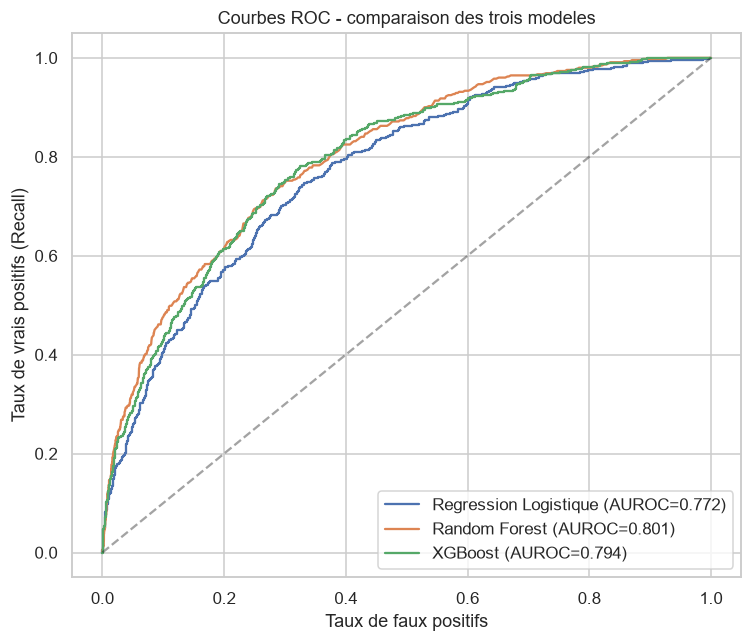
\includegraphics[width=0.62\textwidth]{outputs/courbes_roc.png}
\caption{Courbes \textsc{roc} des trois modèles (échantillon test)}
\label{fig:res-roc}
\end{figure}

\begin{figure}[H]
\centering
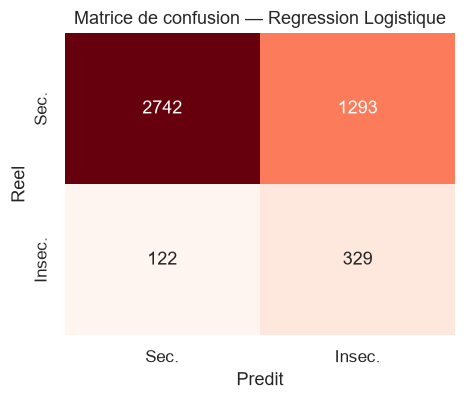
\includegraphics[width=0.45\textwidth]{outputs/matrice_confusion_regression_logistique.png}
\caption{Matrice de confusion de la Régression Logistique (seuil = 0,5)}
\label{fig:res-cm-logit}
\end{figure}

\begin{figure}[H]
\centering
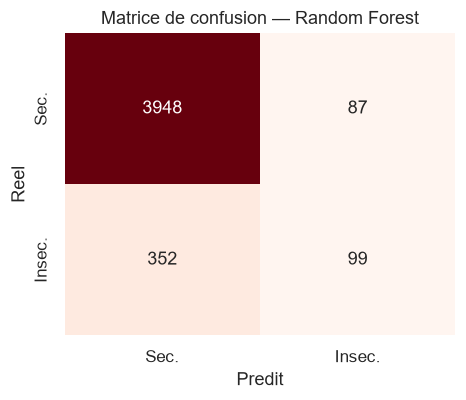
\includegraphics[width=0.45\textwidth]{outputs/matrice_confusion_random_forest.png}
\caption{Matrice de confusion du Random Forest (seuil = 0,5)}
\label{fig:res-cm-rf}
\end{figure}

\begin{figure}[H]
\centering
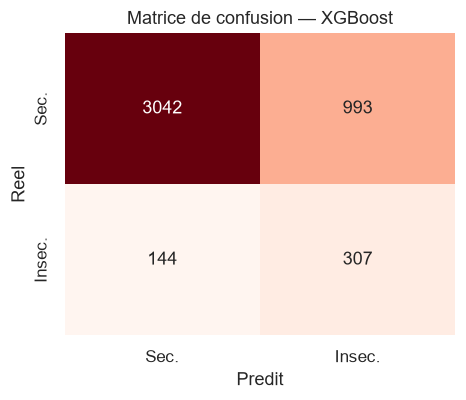
\includegraphics[width=0.45\textwidth]{outputs/matrice_confusion_xgboost.png}
\caption{Matrice de confusion du XGBoost (seuil = 0,5)}
\label{fig:res-cm-xgb}
\end{figure}

\subsubsection{Qualité d'ajustement globale : pseudo-$R^2$ des trois modèles}
\label{sssec:res-pseudor2-comp}

Les trois pseudo-$R^2$ introduits pour le Logit
(Section~\ref{sssec:res-pseudor2}) sont étendus aux deux modèles d'apprentissage
pour comparer la qualité d'ajustement globale des trois approches
(Table~\ref{tab:res-pseudor2}). Une précaution s'impose toutefois : le
\emph{class weighting} \textbf{décalibre volontairement} les probabilités
prédites (il optimise la discrimination, non la vraisemblance), de sorte qu'un
calcul direct sur les probabilités brutes des modèles d'ensemble produirait des
pseudo-$R^2$ négatifs, dénués de sens. Les valeurs inter-modèles sont donc
calculées sur des \textbf{probabilités recalibrées} (régression isotonique
ajustée sur une moitié de l'échantillon test, pseudo-$R^2$ évalué sur l'autre
moitié, sous-ensembles disjoints) ; la valeur classique \emph{in-sample} du
Logit (éq.~14) est rappelée en dernière ligne à titre de référence.

\begin{table}[H]
\centering
\caption{Pseudo-$R^2$ de qualité d'ajustement globale des trois modèles
(probabilités recalibrées sur l'échantillon test, sauf dernière ligne)}
\label{tab:res-pseudor2}
\begin{tabular}{lrrr}
\toprule
\textbf{Modèle} & \textbf{McFadden} & \textbf{Cox-Snell} & \textbf{Nagelkerke} \\
\midrule
Régression Logistique (test recalibré) & 0,147 & 0,091 & 0,191 \\
Random Forest (test recalibré)         & 0,181 & 0,111 & 0,232 \\
XGBoost (test recalibré)               & 0,174 & 0,107 & 0,224 \\
\midrule
Régression Logistique (\emph{in-sample}, éq.~14) & 0,171 & 0,103 & 0,219 \\
\bottomrule
\end{tabular}
\end{table}

Sur des probabilités remises sur un pied de comparabilité, les trois modèles
présentent une qualité d'ajustement globale du même ordre, le
\textbf{Random Forest} (McFadden~=~0,181) et le \textbf{XGBoost}
(0,174) devançant légèrement la régression logistique (0,147). L'ensemble des
pseudo-$R^2$ de McFadden se situe au voisinage du seuil de 0,2 usuellement
associé à un très bon ajustement pour cet indicateur, ce qui conforte, sous un
angle complémentaire à l'\textsc{auroc}, la pertinence des trois modèles et le
léger avantage des méthodes d'ensemble.

\subsubsection{Gestion du déséquilibre : \emph{class weighting} contre \textsc{smote}}

La comparaison prévue à la Section~4.5.2 conforte le choix du
\emph{class weighting} : à hyperparamètres identiques, le XGBoost entraîné sur
données suréchantillonnées par \textsc{smote} obtient une \textsc{auroc}
légèrement inférieure (0,783 contre 0,794) et surtout un \emph{recall}
effondré au seuil de 0,5 (0,118 contre 0,681), rédhibitoire au regard de
l'objectif de détection des ménages vulnérables. Le \emph{class weighting}
présente en outre l'avantage décisif de préserver l'intégration des poids
d'enquête, impossibles à attacher aux observations synthétiques de
\textsc{smote}.

\subsubsection{Analyse de sensibilité à la définition de la variable dépendante}

La hiérarchie des modèles est robuste à la définition de $Y$
(Section~4.2.4) : pour la définition de référence ($\{3,4\}$, prévalence
10,05\,\%) comme pour la définition élargie ($\{2,3,4\}$, 53,20\,\%),
XGBoost domine le Logit (0,794 contre 0,769 et 0,771 contre 0,749
respectivement). Seule la définition stricte ($\{4\}$, 0,83\,\% soit 124~cas)
inverse ponctuellement la hiérarchie (0,814 contre 0,831), inversion à
interpréter avec prudence compte tenu de l'instabilité d'une estimation fondée
sur si peu de cas positifs.

\subsubsection{Calibration des probabilités prédites}

Bruts, les trois modèles sont mal calibrés au sens du test de Hosmer-Lemeshow
($p < 0{,}001$ pour chacun), phénomène attendu : le \emph{class weighting}
optimise la discrimination au détriment de la justesse des probabilités. La
recalibration isotonique du modèle retenu (XGBoost), réalisée sur une moitié de
l'échantillon test et évaluée sur l'autre moitié, corrige ce défaut : le score
de Brier passe de 0,159 à \textbf{0,077} et le test de Hosmer-Lemeshow devient
non significatif ($p = 0{,}479$), indiquant une calibration adéquate
(Figure~\ref{fig:res-calibration}). Le modèle final — XGBoost recalibré — est
donc apte à produire des probabilités interprétables comme des risques réels,
condition posée par l'hypothèse $H_4$ pour le déploiement opérationnel.

\begin{figure}[H]
\centering
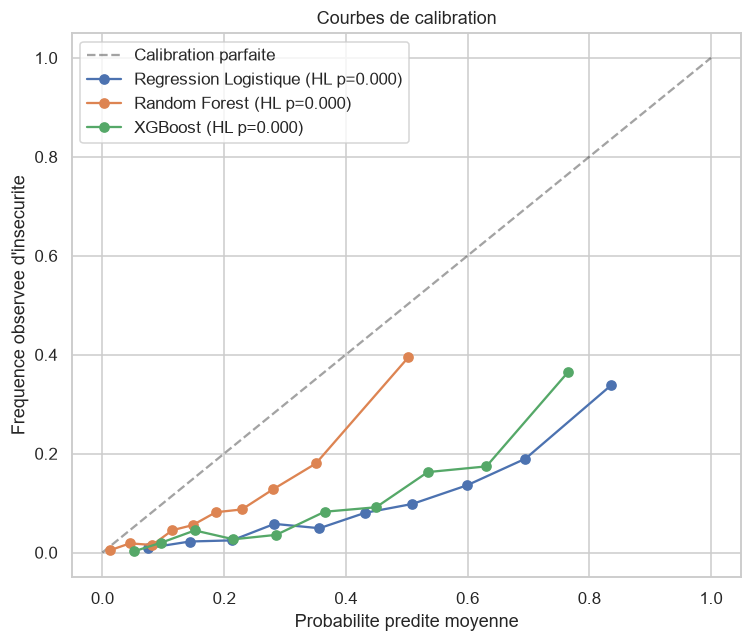
\includegraphics[width=0.62\textwidth]{outputs/calibration.png}
\caption{Courbes de calibration des trois modèles avant recalibration}
\label{fig:res-calibration}
\end{figure}

% ---------------------------------------------------------------------
\subsection{Interprétabilité du modèle retenu : valeurs \textsc{shap}}
\label{ssec:res-shap}

Conformément à la Section~4.7, les valeurs \textsc{shap} ont été calculées pour
les trois modèles (Tree\textsc{shap} pour Random Forest et XGBoost,
Linear\textsc{shap} pour le Logit), sur un échantillon de 1\,200 observations
de l'échantillon test.

\textbf{Importance globale.} Les classements d'importance
(Figure~\ref{fig:res-shap-imp}) convergent avec les déterminants identifiés en
OS1 : les dépenses alimentaires (log), l'accès à l'électricité et le revenu
(log) dominent, suivis de l'indice de qualité du logement et des variables
géographiques (département de l'Atacora). La convergence entre les trois
modèles — pourtant de familles algorithmiques différentes — renforce la
robustesse de ces conclusions.

\textbf{Direction des effets.} Le \emph{summary plot}
(Figure~\ref{fig:res-shap-summary}) confirme le sens des associations : des
dépenses alimentaires faibles, l'absence d'électricité, un revenu faible et un
logement précaire poussent la prédiction vers l'insécurité (valeurs
\textsc{shap} positives), tandis que les niveaux élevés de ces mêmes variables
sont protecteurs.

\textbf{Non-linéarités.} Les \emph{dependence plots} des trois variables les
plus importantes (Figures~\ref{fig:res-shap-dep1}
et~\ref{fig:res-shap-dep2}) révèlent notamment un effet de seuil des dépenses
alimentaires — la contribution au risque devient fortement positive sous un
plancher de dépenses — cohérent avec la non-linéarité détectée par le test de
Box-Tidwell (Section~\ref{ssec:res-bivarie}).

\textbf{Décomposition individuelle.} Les \emph{waterfall plots} de trois
ménages représentatifs illustrent l'usage opérationnel du modèle : pour le
ménage le plus à risque de l'échantillon (probabilité prédite de 0,91 ;
Figure~\ref{fig:res-shap-waterfall}), l'absence de dépenses alimentaires
déclarées (contribution $+0{,}90$ sur l'échelle logit), la résidence dans
l'Atacora ($+0{,}56$), un revenu très faible ($+0{,}16$), l'absence
d'électricité ($+0{,}16$) et l'assistance alimentaire reçue ($+0{,}15$)
constituent l'essentiel du diagnostic. Le
\emph{force plot} interactif du ménage médian, exporté en \textsc{html},
préfigure l'intégration de ces explications individuelles dans l'outil web
(OS4).

\begin{figure}[H]
\centering
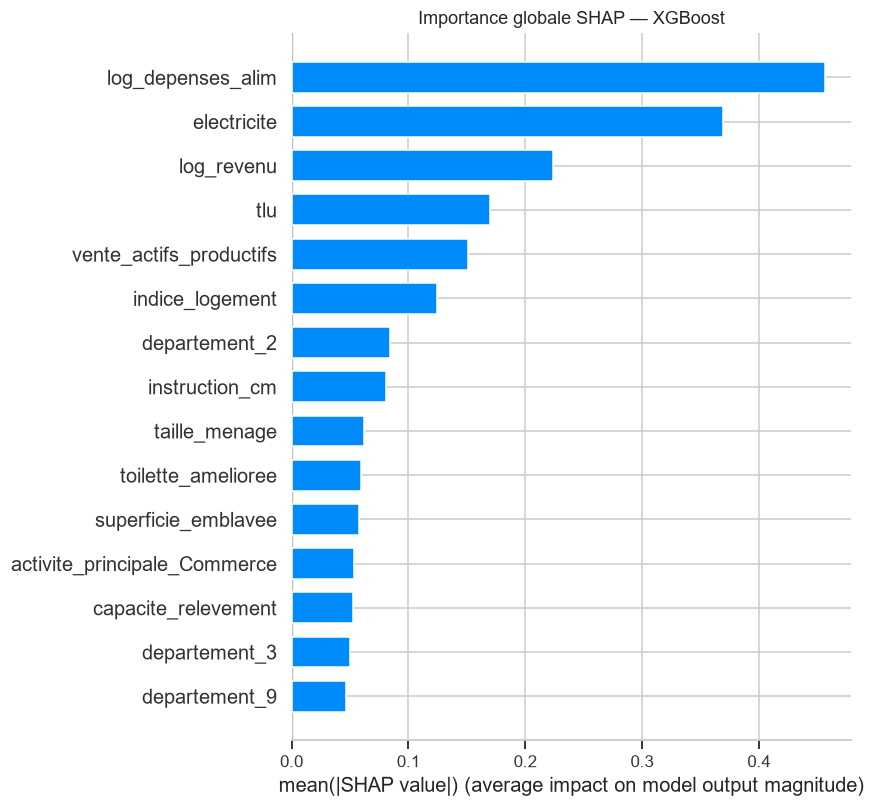
\includegraphics[width=0.72\textwidth]{outputs/shap_importance_xgboost.png}
\caption{Importance globale \textsc{shap} des prédicteurs — XGBoost}
\label{fig:res-shap-imp}
\end{figure}

\begin{figure}[H]
\centering
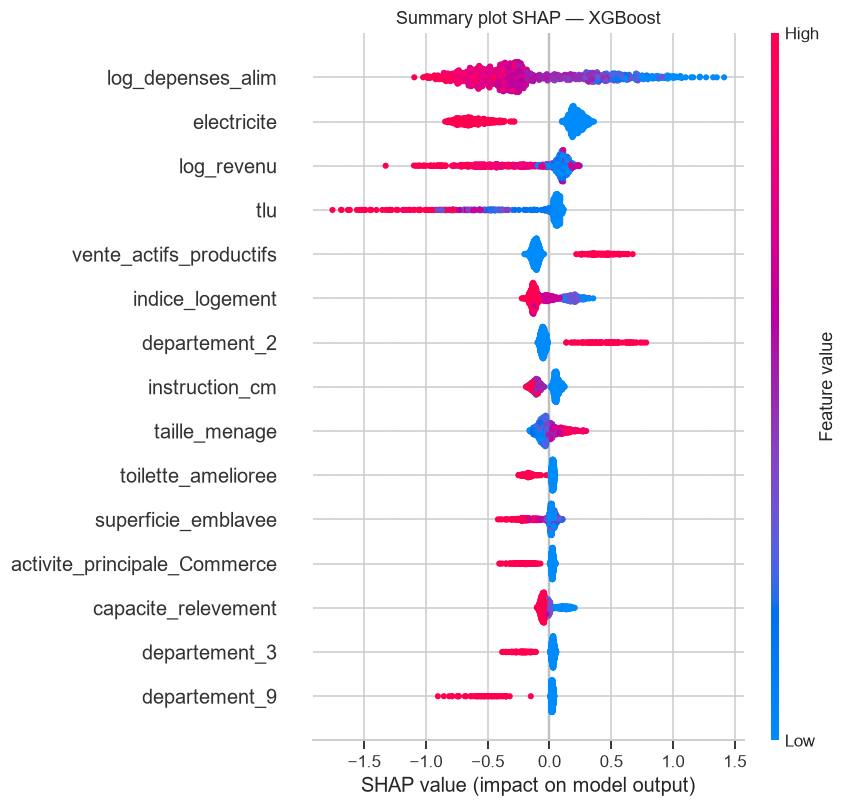
\includegraphics[width=0.72\textwidth]{outputs/shap_summary.png}
\caption{\emph{Summary plot} \textsc{shap} — importance et direction des effets (XGBoost)}
\label{fig:res-shap-summary}
\end{figure}

\begin{figure}[H]
\centering
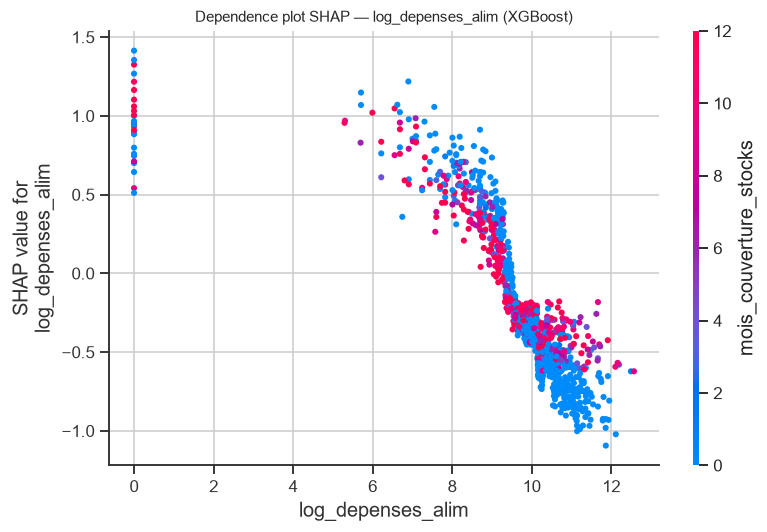
\includegraphics[width=0.6\textwidth]{outputs/shap_dependence_log_depenses_alim.png}
\caption{\emph{Dependence plot} \textsc{shap} des dépenses alimentaires (log)}
\label{fig:res-shap-dep1}
\end{figure}

\begin{figure}[H]
\centering
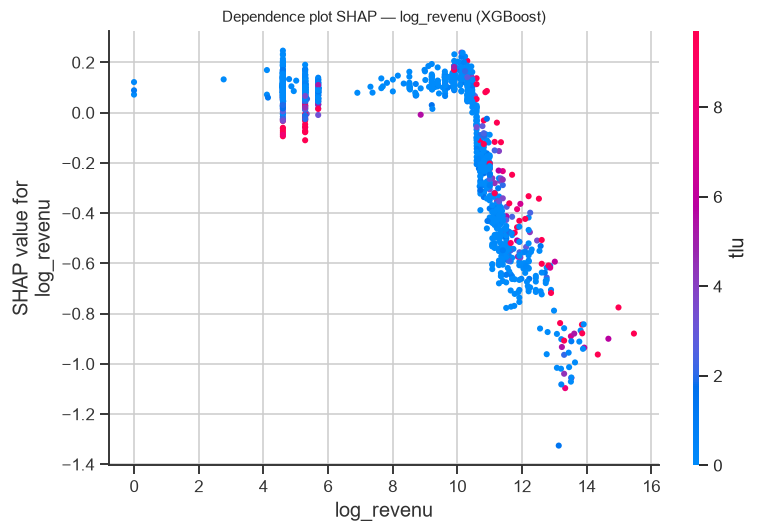
\includegraphics[width=0.6\textwidth]{outputs/shap_dependence_log_revenu.png}
\caption{\emph{Dependence plot} \textsc{shap} du revenu mensuel (log)}
\label{fig:res-shap-dep2}
\end{figure}

\begin{figure}[H]
\centering
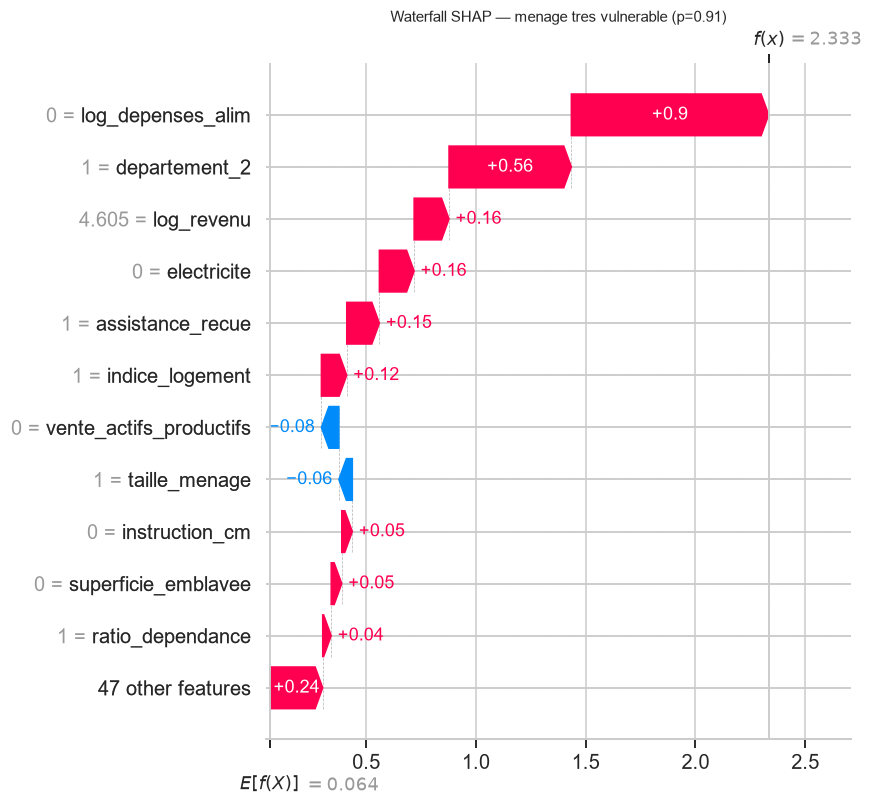
\includegraphics[width=0.72\textwidth]{outputs/shap_waterfall_menage_tres_vulnerable.png}
\caption{\emph{Waterfall plot} \textsc{shap} du ménage le plus vulnérable de l'échantillon
($\hat p = 0{,}91$)}
\label{fig:res-shap-waterfall}
\end{figure}

% ---------------------------------------------------------------------
\subsection{Cartographie communale du risque prédit (OS3)}
\label{ssec:res-os3}

Les probabilités individuelles prédites par le modèle final (XGBoost recalibré)
ont été agrégées par commune avec pondération par les poids d'enquête, puis
jointes au fond de carte des 77~communes (geoBoundaries \textsc{adm}2), avec un
appariement exhaustif (77/77).

\textbf{Autocorrélation spatiale.} L'indice de Moran calculé sur les risques
communaux moyens (matrice de contiguïté de type Queen, standardisée en ligne)
s'établit à $I = 0{,}570$ ($p = 0{,}001$, test par permutations), révélant une
autocorrélation spatiale positive forte et significative : les communes à
risque élevé sont géographiquement groupées. \textbf{L'hypothèse $H_3$ est
confirmée.}

\textbf{Poches de vulnérabilité.} La discrétisation de Jenks en quatre classes
(seuils : 0,08, 0,14 et 0,23) fait apparaître une poche principale de risque
très élevé dans le nord-ouest du pays (département de l'Atacora), et une poche
secondaire dans le centre-sud (Couffo et ouest du Zou)
(Figure~\ref{fig:res-carte}). Les dix communes au risque prédit le plus élevé
sont listées à la Table~\ref{tab:res-communes} : les cinq premières
appartiennent à l'Atacora, Boukoumbé et Toucountouna (39,3\,\% chacune) se
détachant nettement.

\begin{table}[H]
\centering
\caption{Les dix communes au risque prédit d'insécurité alimentaire le plus élevé}
\label{tab:res-communes}
\begin{tabular}{llr}
\toprule
\textbf{Commune} & \textbf{Département} & \textbf{Risque prédit moyen (\%)} \\
\midrule
Boukoumbé    & Atacora & 39,3 \\
Toucountouna & Atacora & 39,3 \\
Tanguiéta    & Atacora & 23,1 \\
Cobly        & Atacora & 22,5 \\
Matéri       & Atacora & 21,5 \\
Agbangnizoun & Zou     & 19,2 \\
Lalo         & Couffo  & 18,9 \\
Natitingou   & Atacora & 18,8 \\
Toviklin     & Couffo  & 17,8 \\
Djakotomey   & Couffo  & 17,4 \\
\bottomrule
\end{tabular}
\end{table}

\begin{figure}[H]
\centering
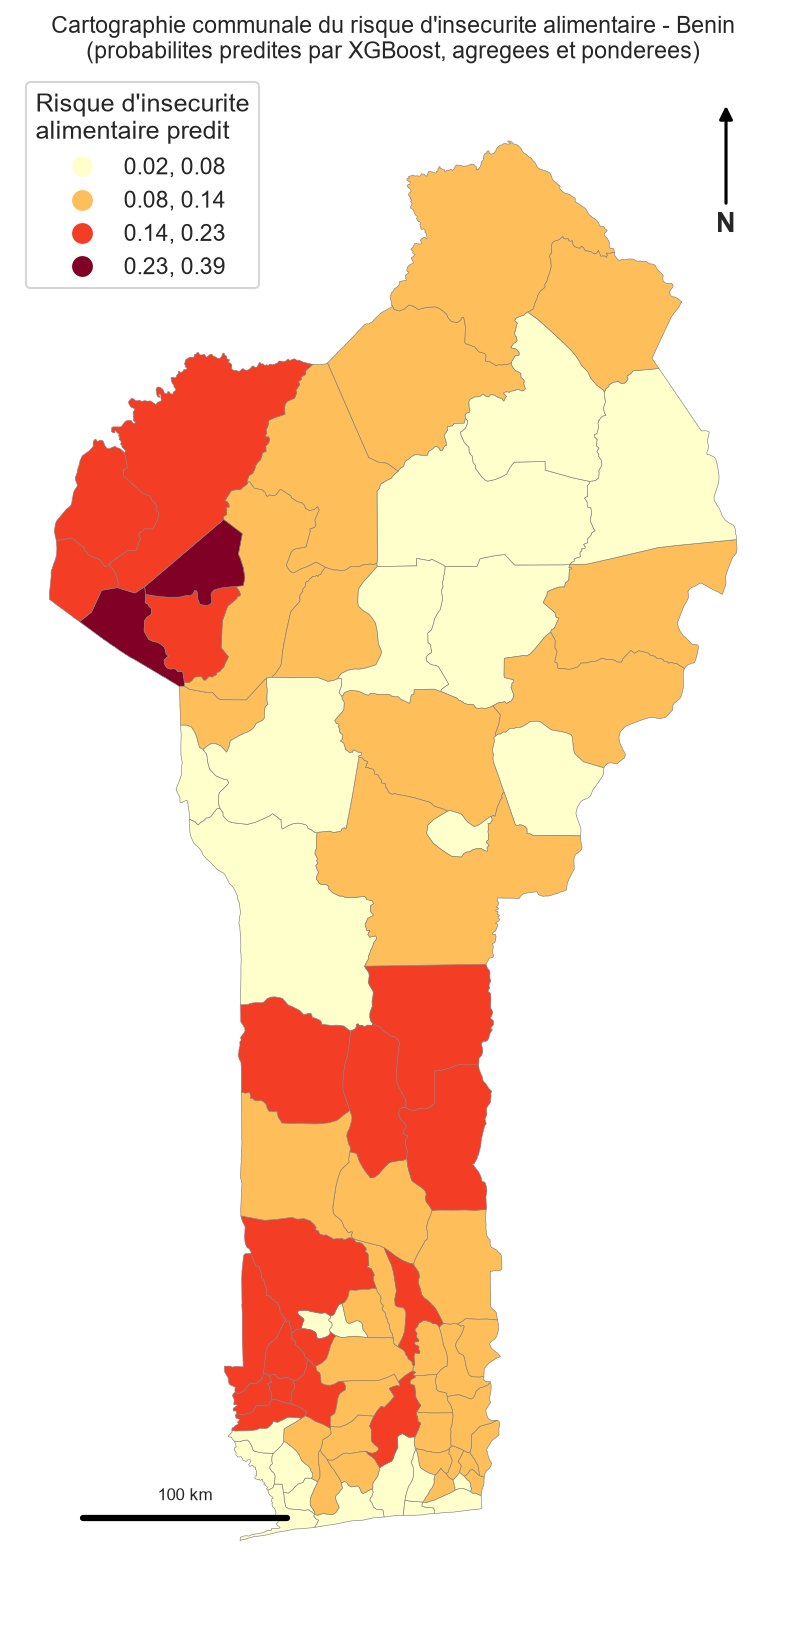
\includegraphics[width=0.8\textwidth]{outputs/carte_risque_communal.png}
\caption{Cartographie communale du risque prédit d'insécurité alimentaire au Bénin
(probabilités du modèle XGBoost, agrégées et pondérées ; discrétisation de Jenks, 4 classes)}
\label{fig:res-carte}
\end{figure}

Ce résultat cartographique converge avec la prévalence départementale observée
(Section~\ref{ssec:res-univarie}) tout en la raffinant à l'échelle communale :
au sein même de l'Atacora, le risque varie du simple au double entre communes,
information directement mobilisable pour le ciblage géographique des
interventions.

% ---------------------------------------------------------------------
\subsection{Produits opérationnels pour l'outil d'aide à la décision (OS4)}
\label{ssec:res-os4}

Le pipeline a produit les artefacts nécessaires au développement de l'outil
d'aide à la décision prévu par l'OS4 :

\begin{itemize}
  \item le \textbf{modèle final sérialisable} (XGBoost recalibré par régression
        isotonique), dont la calibration validée (Brier~=~0,077 ;
        Hosmer-Lemeshow $p = 0{,}479$) autorise des prédictions probabilistes
        fiables sur des ménages hors échantillon au profil similaire à celui de
        l'enquête — condition de l'hypothèse $H_4$ ;
  \item la \textbf{carte interactive} (\texttt{carte\_interactive.html},
        bibliothèque \texttt{folium}) offrant zoom et infobulles communales
        pour la consultation dynamique du risque ;
  \item le \textbf{force plot \textsc{shap} interactif}
        (\texttt{shap\_force\_menage\_median.html}) démontrant la faisabilité
        d'explications individuelles par ménage dans l'application ;
  \item l'\textbf{environnement logiciel figé}
        (\texttt{requirements\_versions.txt}, Section~4.10.1) garantissant la
        reproductibilité du déploiement.
\end{itemize}

Le développement de l'interface applicative elle-même relève des perspectives
et sera discuté au chapitre suivant.

% ---------------------------------------------------------------------
\subsection{Synthèse des résultats au regard des hypothèses de recherche}
\label{ssec:res-hypotheses}

La Table~\ref{tab:res-hypotheses} confronte les résultats obtenus aux quatre
hypothèses formulées au chapitre~2.

\begin{table}[H]
\centering
\caption{Confrontation des résultats aux hypothèses de recherche}
\label{tab:res-hypotheses}
\begin{tabular}{p{0.16\textwidth}p{0.5\textwidth}p{0.24\textwidth}}
\toprule
\textbf{Hypothèse} & \textbf{Résultat empirique} & \textbf{Verdict} \\
\midrule
$H_1$ (OS1) & Éducation (OR = 0,831 ; $p$ = 0,007) et diversification des
revenus (OR = 0,823 ; $p$ = 0,036) significatives ; eau améliorée et résidence
rurale significatives au stade bivarié mais non retenues par le modèle
multivarié (effets absorbés par l'habitat et le département). &
Partiellement validée \\
\addlinespace
$H_2$ (OS2) & AUROC : RF 0,801 $\approx$ XGBoost 0,794 $>$ Logit 0,773 ;
DeLong ML vs Logit significatif ($p \leq 5\times10^{-4}$) ; hiérarchie robuste
aux définitions de $Y$ (hors définition stricte, 124 cas). & Validée \\
\addlinespace
$H_3$ (OS3) & Indice de Moran $I$ = 0,570 ($p$ = 0,001) ; poches concentrées
dans l'Atacora (nord-ouest), secondairement Couffo--Zou. & Validée \\
\addlinespace
$H_4$ (OS4) & Après recalibration isotonique : Brier = 0,077 ;
Hosmer-Lemeshow $p$ = 0,479 ; artefacts opérationnels produits (carte et
explications interactives). & Validée \\
\bottomrule
\end{tabular}
\end{table}

En résumé, l'étude identifie un noyau robuste de déterminants — conditions
économiques du ménage (dépenses, revenu, diversification), capital humain
(instruction, scolarisation), habitat (électricité, qualité du logement) et
ancrage territorial (Atacora) — convergents entre l'approche économétrique
(odds ratios) et l'approche prédictive (valeurs \textsc{shap}) ; elle établit
la supériorité discriminante des algorithmes d'ensemble sur la régression
logistique, sélectionne et calibre un modèle XGBoost opérationnel, et localise
les poches communales de vulnérabilité qui fondent le ciblage géographique des
interventions. Ces résultats sont discutés et mis en perspective au chapitre
suivant.

% ===================== FIN DU CHAPITRE 5 =============================

% =====================================================================

\section{Présentation des résultats}
\label{sec:resultats}

Ce chapitre présente les résultats produits par le pipeline analytique décrit au
chapitre~4, exécuté sous \texttt{Python}~3.11 (\emph{notebook}
\texttt{Pipeline\_Insecurite\_Alimentaire\_Benin.ipynb}, graine aléatoire
\texttt{RANDOM\_STATE = 42}). La présentation suit la progression logique des
objectifs spécifiques : constitution et validation de la variable dépendante
(Section~\ref{ssec:res-echantillon}), analyse descriptive univariée et bivariée
(Sections~\ref{ssec:res-univarie} à~\ref{ssec:res-bivarie}), identification des
déterminants — OS1 (Section~\ref{ssec:res-os1}), comparaison des modèles
prédictifs — OS2 (Section~\ref{ssec:res-os2}), interprétabilité \textsc{shap}
(Section~\ref{ssec:res-shap}), cartographie communale du risque — OS3
(Section~\ref{ssec:res-os3}) et produits opérationnels pour l'outil d'aide à la
décision — OS4 (Section~\ref{ssec:res-os4}). Une synthèse confronte enfin les
résultats aux hypothèses de recherche (Section~\ref{ssec:res-hypotheses}).

% ---------------------------------------------------------------------
\subsection{Constitution de l'échantillon analytique et validation de la variable dépendante}
\label{ssec:res-echantillon}

\subsubsection{Échantillon analytique et prévalence de l'insécurité alimentaire}

La base AGVSAN 2017 compte 14\,952 ménages et 1\,406 variables. La variable
\texttt{Round\_INDICE\_SECAL} est renseignée pour la totalité des ménages :
aucune observation n'a été exclue et l'échantillon analytique est de
$n = 14\,952$. La Table~\ref{tab:res-repartition-y} présente la répartition des
quatre classes \textsc{cari} et les prévalences associées aux trois définitions
de la variable dépendante.

\begin{table}[H]
\centering
\caption{Répartition des classes \textsc{cari} et prévalence de $Y$ selon les trois définitions}
\label{tab:res-repartition-y}
\small\setlength{\tabcolsep}{4pt}
\begin{tabular}{lrr}
\toprule
\textbf{Classe \textsc{cari}} & \textbf{Effectif} & \textbf{\%} \\
\midrule
1 — Sécurité alimentaire          & 6\,998 & 46,80 \\
2 — Sécurité alimentaire limite   & 6\,452 & 43,15 \\
3 — Insécurité modérée            & 1\,378 &  9,22 \\
4 — Insécurité sévère             &    124 &  0,83 \\
\midrule
\textbf{Définition de $Y$}        & \textbf{Prévalence brute} & \textbf{Prévalence pondérée} \\
\midrule
Référence $\{3,4\}$               & 10,05\,\% & 9,66\,\% \\
Stricte $\{4\}$                   &  0,83\,\% & --- \\
Élargie $\{2,3,4\}$               & 53,20\,\% & --- \\
\bottomrule
\end{tabular}
\end{table}

Selon la définition de référence, 1\,502 ménages (10,05\,\% ; 9,66\,\% après
pondération par les poids d'enquête \texttt{weight\_agvsa}) sont en insécurité
alimentaire. Ce fort déséquilibre de classes justifie \emph{a posteriori} la
stratégie de \emph{class weighting} retenue au chapitre~4 (Section~4.5.2). La
prévalence pondérée est nettement différenciée selon le milieu de résidence :
13,03\,\% en milieu rural contre 6,19\,\% en milieu urbain (et 1,52\,\%
seulement à Cotonou), premier indice de la dimension territoriale du phénomène.

\subsubsection{Validation croisée de la classification officielle}

Conformément à la Section~4.2.4, le \textsc{sca} a été reconstruit de manière
indépendante à partir des 18~items bruts de consommation alimentaire
(moyenne~=~49,8 ; médiane~=~50,5 ; étendue 0--112). Sa répartition selon les
seuils standard du \textsc{pam} est : pauvre ($<28$) 1\,435 ménages (9,6\,\%),
limite (28--42) 3\,387 (22,7\,\%), acceptable ($>42$) 10\,130 (67,7\,\%). La
concordance entre le \textsc{sca} reconstruit dichotomisé
($\textsc{sca} \leq 42$) et la classification officielle dichotomisée s'établit
à \textbf{76,1\,\% d'accord global} avec un \textbf{Kappa de Cohen de 0,333},
et la corrélation ordinale entre le \textsc{sca} et la classe \textsc{cari} est
négative et hautement significative (Spearman $\rho = -0{,}371$ ;
$p < 0{,}001$), dans le sens attendu (un \textsc{sca} plus faible correspond à
une classe plus sévère). Cette concordance modérée est conforme à la
littérature : la classification \textsc{cari} officielle combine le \textsc{sca}
avec le \textsc{rcsi} et la part des dépenses alimentaires, de sorte qu'une
concordance parfaite avec le seul \textsc{sca} n'est pas attendue.

La validation par l'indice de stratégies de survie confirme la cohérence de la
variable dépendante : le \textsc{rcsi} moyen est de 18,96 chez les ménages en
insécurité contre 10,79 chez les ménages en sécurité (test unilatéral de
Mann-Whitney, $p = 2{,}2 \times 10^{-66}$).

\paragraph{Limite relative au \textsc{hfias}.} Le score \textsc{hfias} prévu
comme second indicateur de validation (Section~4.2.5) s'est révélé
\textbf{indisponible} dans la base ménage transmise (la colonne \texttt{Q\_9\_05}
du fichier correspond à un autre champ du questionnaire). La validation croisée
repose donc sur le seul \textsc{rcsi}, limite qui sera discutée au chapitre
suivant.

% ---------------------------------------------------------------------
\subsection{Analyse univariée des variables focales}
\label{ssec:res-univarie}

\subsubsection{Situation alimentaire des ménages}

Au niveau national, 89,95\,\% des ménages sont en sécurité alimentaire et
10,05\,\% en insécurité (90,34\,\% et 9,66\,\% après pondération ;
Figure~\ref{fig:res-y-national}). La stratification par département
(Figure~\ref{fig:res-y-departement}) révèle de fortes disparités : la
prévalence brute varie de 1,52\,\% dans le Littoral à \textbf{22,80\,\% dans
l'Atacora}, suivi du Couffo (16,40\,\%), des Collines (15,74\,\%) et du Zou
(11,63\,\%), tous au-dessus de la moyenne nationale. Cette hétérogénéité
géographique, déjà visible au stade descriptif, annonce les résultats de la
cartographie prédictive (Section~\ref{ssec:res-os3}).

\begin{figure}[H]
\centering
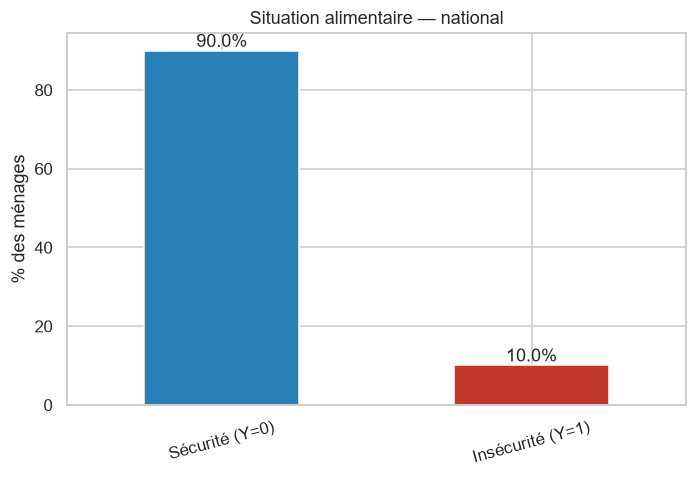
\includegraphics[width=0.62\textwidth]{outputs/univarie_Y_national.png}
\caption{Répartition nationale des ménages selon la situation alimentaire ($Y$)}
\label{fig:res-y-national}
\end{figure}

\begin{figure}[H]
\centering
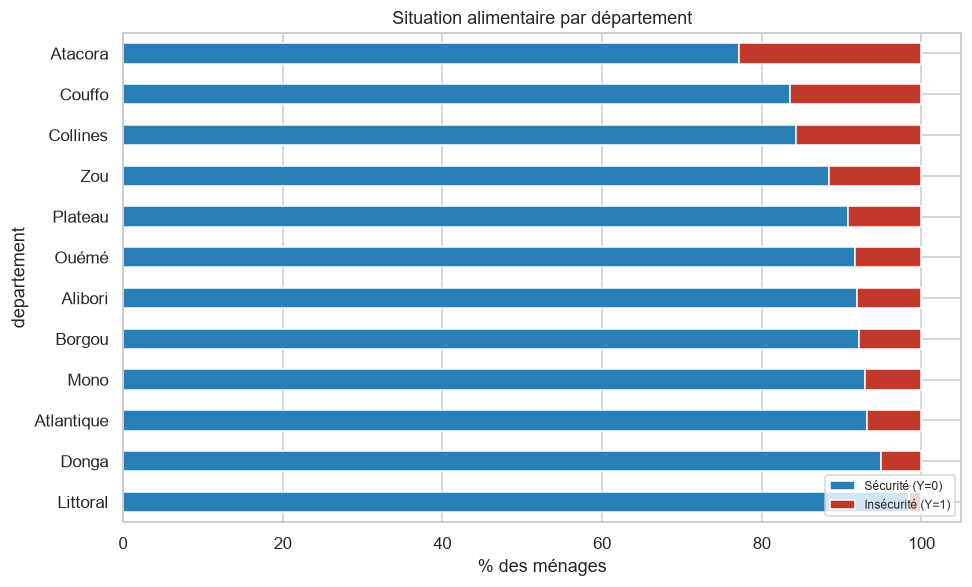
\includegraphics[width=0.85\textwidth]{outputs/univarie_Y_departement.png}
\caption{Situation alimentaire des ménages par département (barres empilées, \% en ligne)}
\label{fig:res-y-departement}
\end{figure}

\subsubsection{Taille des ménages}

La taille moyenne des ménages est de 6,83 personnes (médiane~=~6 ;
écart-type~=~4,57 ; CV~=~66,9\,\%), avec une distribution asymétrique à droite
(skewness~=~2,88) s'étirant jusqu'à 86 personnes
(Figure~\ref{fig:res-taille-hist}). Les ménages ruraux sont en moyenne plus
grands que les ménages urbains (7,2 contre 6,4 personnes ;
Figure~\ref{fig:res-taille-box}), les percentiles extrêmes confirmant cet écart
($P_{90}$ de 13 en milieu rural contre 11 en milieu urbain).

\begin{figure}[H]
\centering
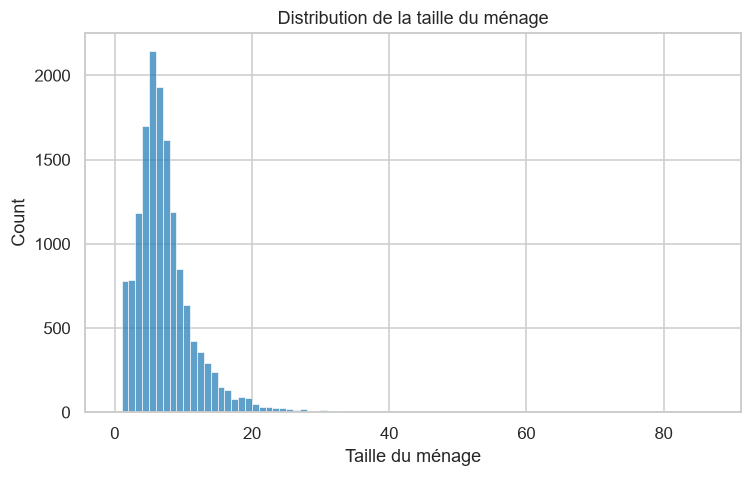
\includegraphics[width=0.62\textwidth]{outputs/univarie_taille_hist.png}
\caption{Distribution de la taille des ménages}
\label{fig:res-taille-hist}
\end{figure}

\begin{figure}[H]
\centering
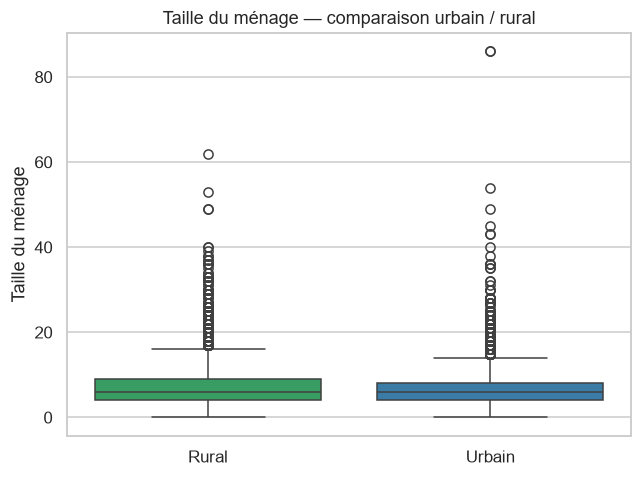
\includegraphics[width=0.55\textwidth]{outputs/univarie_taille_boxplot.png}
\caption{Taille des ménages : comparaison urbain / rural (boîtes à moustaches)}
\label{fig:res-taille-box}
\end{figure}

\subsubsection{Revenu mensuel}

Le revenu mensuel déclaré présente l'asymétrie extrême caractéristique des
données de revenu : moyenne de 68\,105 \textsc{fcfa} pour une médiane de
15\,000 \textsc{fcfa}, écart-type de 217\,941 \textsc{fcfa}
(CV~=~320\,\%), skewness de 11,06 et kurtosis de 181,8
(Figure~\ref{fig:res-revenu-brut}). La transformation logarithmique
$\ln(\text{revenu}+1)$ retenue pour la modélisation (Section~4.3.3) ramène la
skewness à $-0{,}06$, soit une distribution quasi symétrique
(Figure~\ref{fig:res-revenu-log}), ce qui valide empiriquement ce choix
méthodologique.

\begin{figure}[H]
\centering
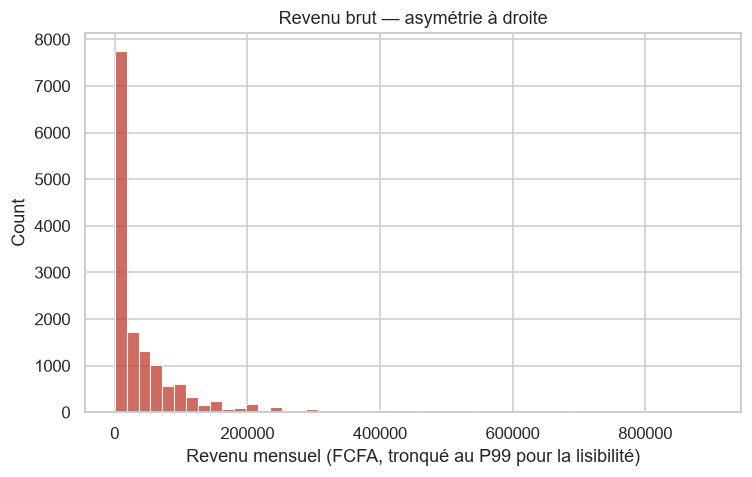
\includegraphics[width=0.62\textwidth]{outputs/univarie_revenu_brut.png}
\caption{Distribution du revenu mensuel brut (\textsc{fcfa}, tronqué au $P_{99}$)}
\label{fig:res-revenu-brut}
\end{figure}

\begin{figure}[H]
\centering
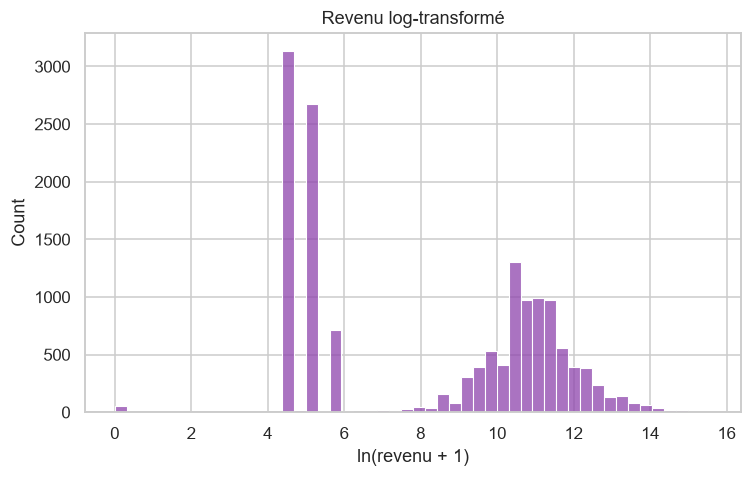
\includegraphics[width=0.62\textwidth]{outputs/univarie_revenu_log.png}
\caption{Distribution du revenu log-transformé $\ln(\text{revenu}+1)$}
\label{fig:res-revenu-log}
\end{figure}

\subsubsection{Âge du chef de ménage}

L'âge moyen du chef de ménage est de 47,1 ans (médiane~=~45 ;
écart-type~=~15,0 ; étendue 16--100 ans), avec une asymétrie modérée
(skewness~=~0,70 ; Figure~\ref{fig:res-age}). La répartition par tranches
usuelles est la suivante : moins de 30~ans, 8,94\,\% ; 30--44~ans, 37,22\,\% ;
45--59~ans, 32,30\,\% ; 60~ans et plus, 21,54\,\%.

\begin{figure}[H]
\centering
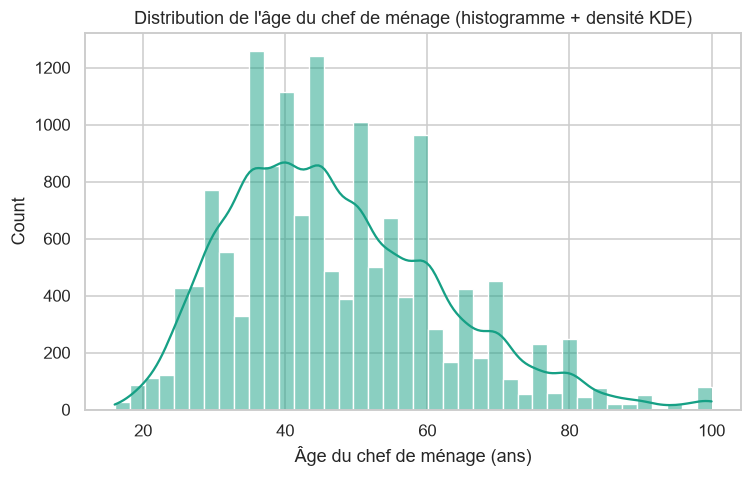
\includegraphics[width=0.62\textwidth]{outputs/univarie_age.png}
\caption{Distribution de l'âge du chef de ménage (histogramme et densité à noyau)}
\label{fig:res-age}
\end{figure}

\subsubsection{Niveau d'instruction du chef de ménage}

Plus de la moitié des chefs de ménage (51,22\,\%) n'ont aucune instruction
formelle ; viennent ensuite le primaire (22,59\,\%), le secondaire (17,04\,\%),
le supérieur (4,47\,\%), l'alphabétisation (3,36\,\%), l'école coranique
(1,17\,\%) et le cursus arabe (0,06\,\%) (Figure~\ref{fig:res-instruction}).
Après recodage en trois niveaux (Table~5 du chapitre~4), la répartition est :
\emph{Aucun/informel} 55,89\,\%, \emph{Primaire} 22,59\,\%,
\emph{Secondaire et plus} 21,52\,\%.

\begin{figure}[H]
\centering
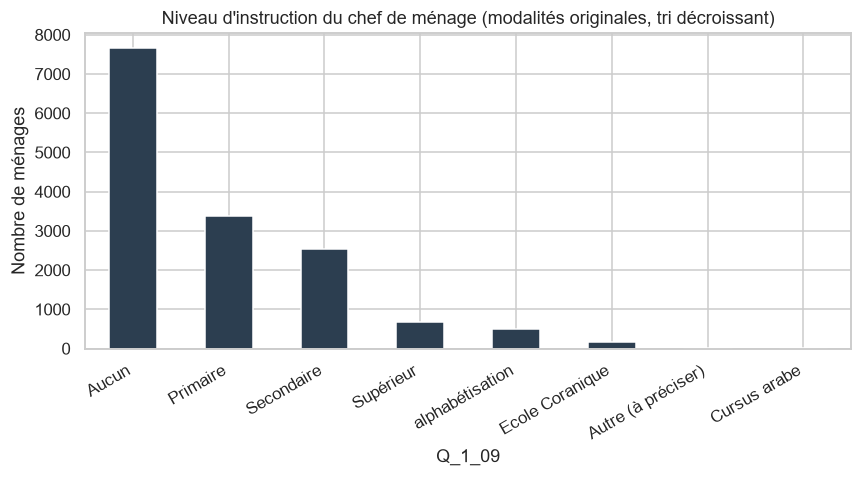
\includegraphics[width=0.72\textwidth]{outputs/univarie_instruction.png}
\caption{Niveau d'instruction du chef de ménage (modalités originales, tri décroissant)}
\label{fig:res-instruction}
\end{figure}

\subsubsection{Accès au crédit}

Un peu plus du quart des ménages (25,79\,\% ; 26,26\,\% pondéré) a contracté un
emprunt au cours des douze derniers mois. L'accès au crédit est légèrement plus
fréquent en milieu rural (27,31\,\%) qu'en milieu urbain (23,99\,\%)
(Figure~\ref{fig:res-credit-univ}).

\begin{figure}[H]
\centering
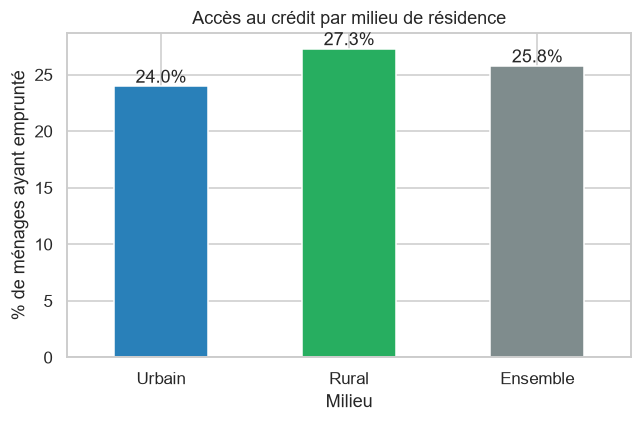
\includegraphics[width=0.55\textwidth]{outputs/univarie_credit.png}
\caption{Proportion de ménages ayant accès au crédit, par milieu de résidence}
\label{fig:res-credit-univ}
\end{figure}

% ---------------------------------------------------------------------
\subsection{Tests de normalité des variables continues}
\label{ssec:res-normalite}

La Table~\ref{tab:res-normalite} rapporte les tests de normalité prévus à la
Section~4.4.3. Pour les quatre variables continues focales, l'hypothèse de
normalité est rejetée par le test de Kolmogorov-Smirnov comme par celui de
Shapiro-Wilk ($p < 0{,}001$ dans tous les cas), conclusion corroborée par les
coefficients de forme et par les QQ-plots
(Figures~\ref{fig:res-qq-taille} et~\ref{fig:res-qq-age}). Conformément à la
règle de décision du chapitre~4 — et en tenant compte de la puissance très
élevée de ces tests avec $n \approx 15\,000$ — l'analyse bivariée recourt
systématiquement au test non paramétrique de Mann-Whitney pour les variables
continues.

\begin{table}[H]
\centering
\caption{Tests de normalité des variables continues focales ($n = 14\,952$)}
\label{tab:res-normalite}
\small\setlength{\tabcolsep}{4pt}
\begin{tabular}{lrrrrrl}
\toprule
\textbf{Variable} & \textbf{KS $D_n$} & \textbf{KS $p$} & \textbf{Shapiro $W$} & \textbf{Skew.} & \textbf{Kurt.} & \textbf{Conclusion} \\
\midrule
Taille du ménage        & 0,164 & $<0{,}001$ & 0,813 &  2,88 & 22,24  & Normalité rejetée \\
Revenu brut (\textsc{fcfa}) & 0,377 & $<0{,}001$ & 0,267 & 11,06 & 181,85 & Normalité rejetée \\
$\ln(\text{revenu}+1)$  & 0,239 & $<0{,}001$ & 0,848 & $-0{,}06$ & $-1{,}54$ & Normalité rejetée \\
Âge du chef de ménage   & 0,092 & $<0{,}001$ & 0,969 &  0,70 & 0,33   & Normalité rejetée \\
\bottomrule
\end{tabular}
\end{table}

\begin{figure}[H]
\centering
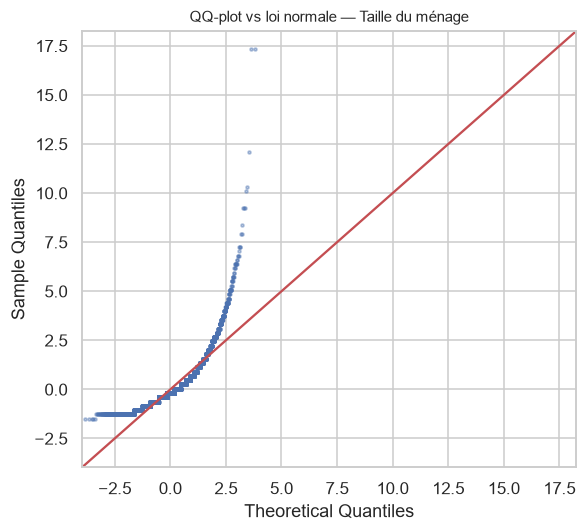
\includegraphics[width=0.48\textwidth]{outputs/normalite_qq_taille.png}
\caption{QQ-plot de la taille du ménage contre la loi normale standard}
\label{fig:res-qq-taille}
\end{figure}

\begin{figure}[H]
\centering
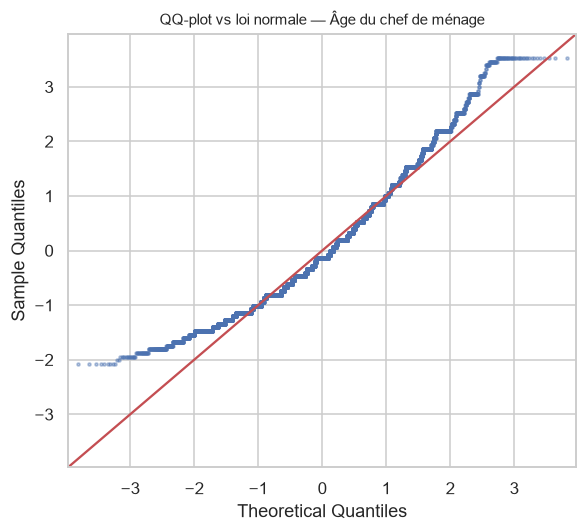
\includegraphics[width=0.48\textwidth]{outputs/normalite_qq_age.png}
\caption{QQ-plot de l'âge du chef de ménage contre la loi normale standard}
\label{fig:res-qq-age}
\end{figure}

% ---------------------------------------------------------------------
\subsection{Analyse bivariée et tests pré-estimation}
\label{ssec:res-bivarie}

\subsubsection{Variables focales croisées avec la situation alimentaire}

La Table~\ref{tab:res-bivarie-focales} synthétise les tests bivariés conduits
selon le canevas de la Section~4.4.4 (le test de Levene ayant orienté, avec le
rejet de la normalité, vers le test de Mann-Whitney pour les continues).

\begin{table}[H]
\centering
\caption{Analyse bivariée des variables focales $\times$ situation alimentaire ($Y$)}
\label{tab:res-bivarie-focales}
\small\setlength{\tabcolsep}{3.5pt}
\begin{tabular}{lllrl}
\toprule
\textbf{Variable} & \textbf{Test} & \textbf{Statistique} & \textbf{$p$-valeur} & \textbf{Conclusion} \\
\midrule
Taille du ménage        & Mann-Whitney & $U = 9\,667\,365{,}5$  & 0,006                 & Significatif \\
$\ln(\text{revenu}+1)$  & Mann-Whitney & $U = 8\,119\,697{,}0$  & $2{,}7\times10^{-36}$ & Significatif \\
Âge du chef de ménage   & Mann-Whitney & $U = 10\,613\,702{,}0$ & 0,001                 & Significatif \\
Niveau d'instruction    & $\chi^2$ (ddl = 2) & $\chi^2 = 226{,}06$ ; $V = 0{,}123$ & $8{,}2\times10^{-50}$ & Significatif \\
Accès au crédit         & $\chi^2$ (2$\times$2) & $\chi^2 = 0{,}013$ ; OR = 0,991 & 0,908 & \textbf{Non significatif} \\
\bottomrule
\end{tabular}
\end{table}

Quatre enseignements ressortent de cette analyse.

\textbf{(i) Le revenu est le facteur focal le plus discriminant.} Le revenu
log-transformé des ménages en insécurité est très inférieur à celui des ménages
en sécurité (médianes de 5,70 contre 9,63 sur l'échelle log, soit environ 297
contre 15\,198 \textsc{fcfa} sur l'échelle brute ;
$p = 2{,}7\times10^{-36}$ ; Figure~\ref{fig:res-box-revenu}), résultat cohérent
avec l'approche des pièges à pauvreté discutée au chapitre~3.

\textbf{(ii) Le gradient d'instruction est net et monotone.} La prévalence de
l'insécurité décroît régulièrement avec le niveau d'instruction du chef de
ménage : 13,17\,\% (\emph{Aucun/informel}), 7,73\,\% (\emph{Primaire}),
4,35\,\% (\emph{Secondaire et plus}) ($\chi^2(2) = 226{,}06$ ;
$V$ de Cramér~=~0,123 ; Figure~\ref{fig:res-biv-instruction}), conformément à
la littérature.

\textbf{(iii) Deux résultats vont à rebours de l'intuition.} D'une part, les
ménages en insécurité sont en moyenne légèrement \emph{plus petits} que les
ménages en sécurité (6,54 contre 6,87 personnes ; $p = 0{,}006$ ;
Figure~\ref{fig:res-box-taille}). D'autre part, la relation entre l'âge du chef
de ménage et l'insécurité est en U : la prévalence est plus élevée aux deux
extrémités de la distribution (11,23\,\% avant 30~ans et 12,79\,\% à 60~ans et
plus, contre 8,97\,\% et 9,13\,\% pour les tranches intermédiaires), les
moyennes différant significativement (48,69 contre 46,93 ans ; $p = 0{,}001$ ;
Figure~\ref{fig:res-box-age}).

\textbf{(iv) L'accès au crédit n'est pas associé au statut alimentaire.} La
prévalence de l'insécurité est quasi identique chez les ménages emprunteurs
(9,98\,\%) et non emprunteurs (10,07\,\%), et l'odds ratio brut est nul au sens
statistique (OR~=~0,991 ; IC à 95\,\% $[0{,}877\,;\,1{,}120]$ ; $p = 0{,}908$ ;
Figure~\ref{fig:res-biv-credit}). Ce résultat nul, contraire à l'hypothèse
d'un rôle protecteur du crédit, sera repris dans la discussion.

\begin{figure}[H]
\centering
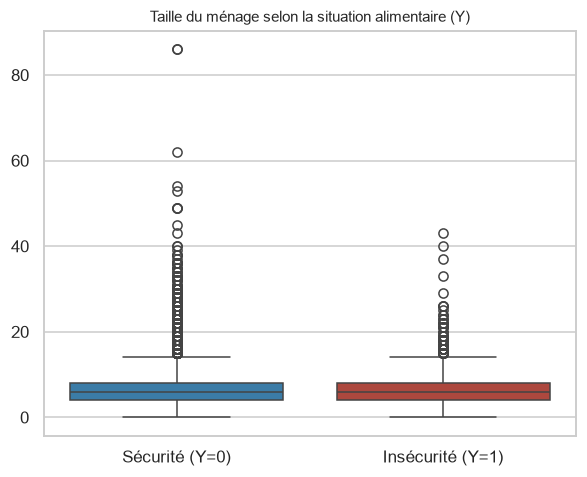
\includegraphics[width=0.5\textwidth]{outputs/bivarie_boxplot_taille.png}
\caption{Taille du ménage selon la situation alimentaire}
\label{fig:res-box-taille}
\end{figure}

\begin{figure}[H]
\centering
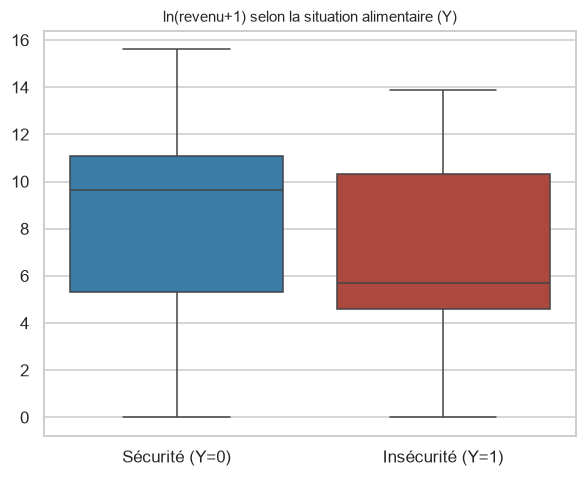
\includegraphics[width=0.5\textwidth]{outputs/bivarie_boxplot_revenu.png}
\caption{Revenu log-transformé selon la situation alimentaire}
\label{fig:res-box-revenu}
\end{figure}

\begin{figure}[H]
\centering
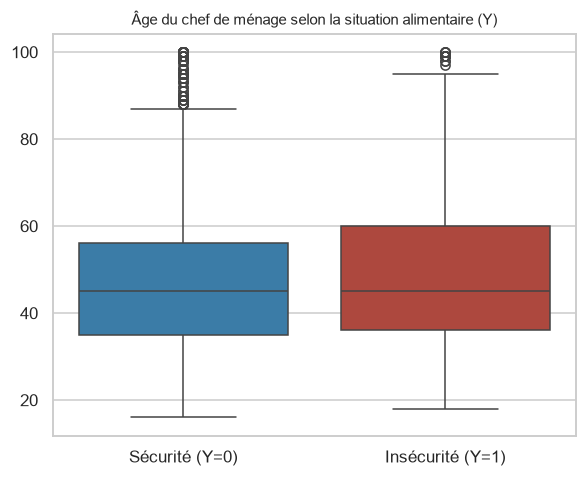
\includegraphics[width=0.5\textwidth]{outputs/bivarie_boxplot_age.png}
\caption{Âge du chef de ménage selon la situation alimentaire}
\label{fig:res-box-age}
\end{figure}

\begin{figure}[H]
\centering
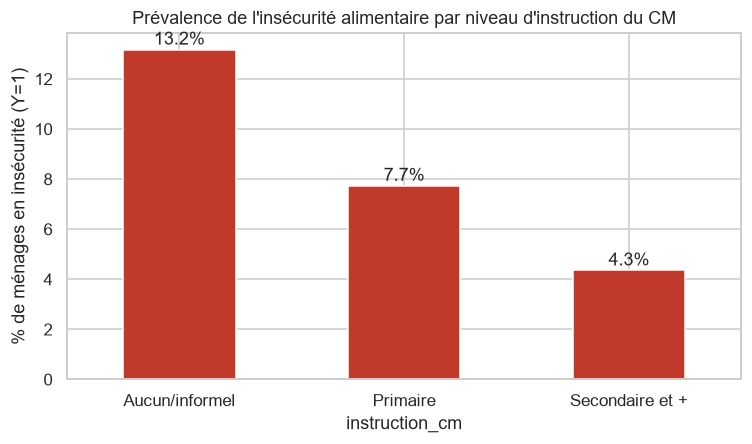
\includegraphics[width=0.62\textwidth]{outputs/bivarie_instruction.png}
\caption{Prévalence de l'insécurité alimentaire selon le niveau d'instruction du chef de ménage}
\label{fig:res-biv-instruction}
\end{figure}

\begin{figure}[H]
\centering
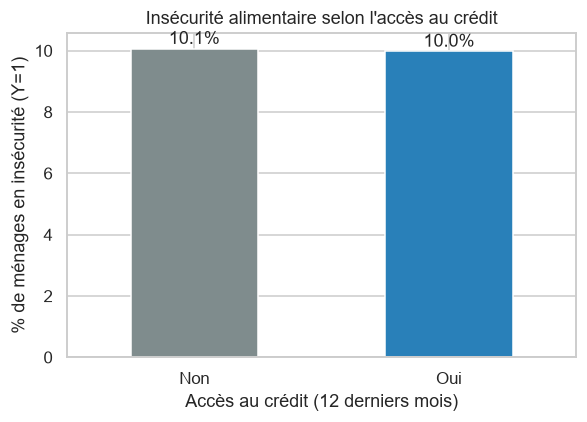
\includegraphics[width=0.5\textwidth]{outputs/bivarie_credit.png}
\caption{Prévalence de l'insécurité alimentaire selon l'accès au crédit}
\label{fig:res-biv-credit}
\end{figure}

\subsubsection{Tests bivariés étendus et correction pour comparaisons multiples}

L'analyse a été étendue à l'ensemble des variables indépendantes retenues
(Table~10 du chapitre~4), soit 22~tests, avec correction de Benjamini-Hochberg
(contrôle du \textsc{fdr}). Après correction, \textbf{20 des 22 variables
demeurent significativement associées} au statut alimentaire au seuil de
5\,\% ; seules la possession de bétail (\textsc{tlu}, $p_{aj} = 0{,}709$) et
l'accès au crédit ($p_{aj} = 0{,}908$) ne le sont pas. Les associations les
plus fortes concernent, par ordre de $p$-valeur ajustée croissante : les
dépenses alimentaires (log), l'accès à l'électricité ($V = 0{,}169$), le
département ($V = 0{,}179$), l'indice de qualité du logement, le niveau
d'instruction, le milieu de résidence ($V = 0{,}115$) et le revenu (log). La
nouvelle variable « mois de couverture des stocks » est également associée au
statut alimentaire ($p_{aj} < 0{,}001$), les ménages en insécurité déclarant
paradoxalement une couverture médiane plus longue (2~mois contre 0), reflet de
leur profil plus agricole.

\subsubsection{Multicolinéarité et linéarité dans le logit}

Aucune colinéarité problématique n'est détectée parmi les prédicteurs continus :
tous les \textsc{vif} sont inférieurs à 2 (maximum : diversification des
revenus, \textsc{vif} = 1,82). Pour les variables polytomiques, le \textsc{gvif}
de Fox et Monette conduit à la même conclusion
(Table~\ref{tab:res-gvif}) : la valeur normalisée maximale
$\text{GVIF}^{1/(2\,\text{ddl})} = 1{,}78$ (type de choc) reste sous le seuil
de $\sqrt{5} \approx 2{,}24$. L'ensemble des prédicteurs peut donc être
conservé dans le modèle logistique.

\begin{table}[H]
\centering
\caption{GVIF des variables polytomiques (Fox et Monette, 1992)}
\label{tab:res-gvif}
\begin{tabular}{lrrr}
\toprule
\textbf{Variable} & \textbf{ddl} & \textbf{GVIF} & \textbf{GVIF$^{1/(2\,\text{ddl})}$} \\
\midrule
Statut matrimonial    &  5 &   2,155 & 1,080 \\
Département           & 11 &   6,231 & 1,087 \\
Activité principale   &  5 &   5,163 & 1,178 \\
Type de choc          &  4 & 102,411 & 1,784 \\
\bottomrule
\end{tabular}
\end{table}

Le test de Box-Tidwell (Section~4.5.3) conclut à une linéarité acceptable dans
le logit pour l'âge ($p = 0{,}61$), la taille du ménage ($p = 0{,}21$) et le
ratio de dépendance ($p = 0{,}11$) ; seules les dépenses alimentaires (log)
présentent une non-linéarité significative ($p = 3{,}9\times10^{-18}$),
qu'avec $n \approx 15\,000$ il convient de relativiser et que les modèles
d'arbres (Random Forest, XGBoost), non paramétriques, capturent par
construction.

\subsubsection{Robustesse au plan de sondage : analyse pondérée design-based}
\label{sssec:res-ponderee}

Conformément à la Section~4.5.1, les statistiques descriptives et les tests
bivariés ont été recalculés en tenant compte du plan de sondage complexe
(poids \texttt{weight\_agvsa}, grappes en unités primaires, strates
reconstruites «~département~$\times$~milieu~») au moyen du package
\texttt{samplics} (linéarisation de Taylor). Les proportions et moyennes
pondérées sont assorties d'un intervalle de confiance design-based
(Table~\ref{tab:res-pondere-uni}). Pour les variables continues et binaires,
l'association avec $Y$ est testée par comparaison design-based des
moyennes/proportions par domaine ; pour les variables polytomiques, pour
lesquelles le test de Rao-Scott n'était pas exploitable dans la version
disponible du package, le test est calculé par repondération simple des
effectifs, conformément à la limite reconnue au chapitre~4.

\begin{table}[H]
\centering
\caption{Statistiques univariées pondérées design-based (intervalles de confiance
à 95\,\% de Taylor)}
\label{tab:res-pondere-uni}
\small\setlength{\tabcolsep}{5pt}
\begin{tabular}{llr}
\toprule
\textbf{Variable} & \textbf{Paramètre} & \textbf{Estimation [IC à 95\,\%]} \\
\midrule
Insécurité alimentaire ($Y=1$) & proportion & 9,66\,\% [8,98 ; 10,37] \\
Accès à l'électricité          & proportion & 41,62\,\% [39,49 ; 43,78] \\
Eau améliorée                  & proportion & 74,46\,\% [72,54 ; 76,30] \\
Accès au crédit                & proportion & 26,26\,\% [24,93 ; 27,64] \\
Résidence rurale               & proportion & 50,70\,\% [49,22 ; 52,17] \\
Taille du ménage               & moyenne    & 6,50 [6,40 ; 6,60] \\
Âge du chef de ménage          & moyenne    & 46,94 [46,58 ; 47,29] \\
$\ln(\text{revenu}+1)$         & moyenne    & 8,29 [8,15 ; 8,42] \\
\bottomrule
\end{tabular}
\end{table}

La prise en compte du plan de sondage \textbf{ne modifie pas les conclusions
qualitatives pour 20 des 22 variables} testées : les associations mises en
évidence au stade non pondéré (Section~\ref{ssec:res-bivarie}) demeurent
significatives en analyse pondérée. Deux variables font toutefois exception, ce
qui souligne l'intérêt de l'approche design-based :

\begin{itemize}
  \item la \textbf{possession de bétail} (\textsc{tlu}), non significative en
        non pondéré ($p = 0{,}68$), devient hautement significative en pondéré
        ($p = 4{,}4\times10^{-10}$) : l'élevage, concentré dans des strates du
        Nord fortement pondérées, apparaît alors nettement associé au statut
        alimentaire ;
  \item la \textbf{taille du ménage}, significative en non pondéré ($p = 0{,}006$),
        ne l'est plus en pondéré ($p = 0{,}159$) : l'écart observé sur
        l'échantillon brut ne résiste pas à la représentativité du plan de
        sondage.
\end{itemize}

Ces deux nuances mises à part, la convergence des deux approches conforte la
robustesse des associations décrites, et l'analyse pondérée fournit les
prévalences représentatives au niveau national mobilisées dans la discussion.

% ---------------------------------------------------------------------
\subsection{Déterminants du risque d'insécurité alimentaire (OS1)}
\label{ssec:res-os1}

La partition stratifiée 70/30 a produit un échantillon d'apprentissage de
10\,466 ménages (10,0\,\% de $Y=1$ ; 750~grappes) et un échantillon test de
4\,486 ménages (10,1\,\% ; 749~grappes). La régression logistique pénalisée
Elastic-Net ($\ell_1$-ratio~=~1,0, soit une pénalisation \textsc{lasso} pure ;
$C \approx 0{,}046$, sélectionnés par validation croisée) sert de modèle
prédictif ; l'inférence sur les déterminants repose sur
le \textsc{glm} binomial non pénalisé, pondéré par les poids d'enquête
normalisés, avec erreurs-types robustes en grappes (Section~4.5.3). La
Table~\ref{tab:res-or} présente les odds ratios significatifs au seuil de
5\,\%, classés en facteurs aggravants et protecteurs.

\begin{table}[H]
\centering
\caption{Déterminants significatifs de l'insécurité alimentaire — odds ratios du \textsc{glm}
binomial pondéré, erreurs-types robustes en grappes (échantillon d'apprentissage, $n = 10\,466$)}
\label{tab:res-or}
\begin{tabular}{lrrr}
\toprule
\textbf{Variable} & \textbf{OR} & \textbf{IC à 95\,\%} & \textbf{$p$-valeur} \\
\midrule
\multicolumn{4}{l}{\emph{Facteurs aggravants (OR $>$ 1)}} \\
\midrule
Vente d'actifs productifs (stratégie de crise) & 2,071 & [1,640 ; 2,615] & $<0{,}001$ \\
Département de l'Atacora (réf. : Atlantique)   & 2,285 & [1,451 ; 3,600] & $<0{,}001$ \\
Pratique de l'agriculture                      & 2,240 & [1,429 ; 3,512] & $<0{,}001$ \\
Assistance alimentaire reçue                   & 1,720 & [1,280 ; 2,313] & $<0{,}001$ \\
Taille du ménage (par personne suppl.)         & 1,031 & [1,010 ; 1,052] & 0,004 \\
\midrule
\multicolumn{4}{l}{\emph{Facteurs protecteurs (OR $<$ 1)}} \\
\midrule
Dépenses alimentaires (log)                    & 0,852 & [0,821 ; 0,883] & $<0{,}001$ \\
Accès à l'électricité                          & 0,495 & [0,385 ; 0,636] & $<0{,}001$ \\
Indice de qualité du logement (0--3)           & 0,805 & [0,734 ; 0,883] & $<0{,}001$ \\
Superficie emblavée (classe)                   & 0,840 & [0,777 ; 0,908] & $<0{,}001$ \\
Possession de bétail (\textsc{tlu})            & 0,929 & [0,895 ; 0,964] & $<0{,}001$ \\
Sécurité foncière                              & 0,666 & [0,502 ; 0,884] & 0,005 \\
Activité principale : commerce (réf. : agric.) & 0,630 & [0,457 ; 0,869] & 0,005 \\
Niveau d'instruction du CM (par niveau)        & 0,831 & [0,726 ; 0,951] & 0,007 \\
Taux de scolarisation des enfants              & 0,618 & [0,430 ; 0,889] & 0,009 \\
Département du Mono                            & 0,401 & [0,197 ; 0,816] & 0,012 \\
Toilettes améliorées                           & 0,697 & [0,525 ; 0,924] & 0,012 \\
Département de la Donga                        & 0,485 & [0,262 ; 0,895] & 0,021 \\
Département du Littoral                        & 0,442 & [0,209 ; 0,935] & 0,033 \\
Capacité de relèvement après choc              & 0,828 & [0,695 ; 0,988] & 0,036 \\
Diversification des revenus (par source)       & 0,823 & [0,686 ; 0,987] & 0,036 \\
Revenu mensuel (log)                           & 0,966 & [0,935 ; 0,999] & 0,041 \\
\bottomrule
\end{tabular}
\end{table}

Trois lectures se dégagent de ce tableau.

\textbf{Le capital physique et financier protège.} L'accès à l'électricité
divise par deux la cote d'insécurité (OR~=~0,495), et chaque point de l'indice
de qualité du logement la réduit de 20\,\% environ ; le niveau des dépenses
alimentaires, le revenu et la diversification des sources de revenus jouent
dans le même sens, de même que le capital humain (instruction du chef de
ménage, scolarisation des enfants) et le capital naturel sécurisé (superficie
emblavée, sécurité foncière, bétail).

\textbf{Les marqueurs de vulnérabilité en cours sont aggravants.} La vente
d'actifs productifs — stratégie d'adaptation destructrice — double la cote
d'insécurité (OR~=~2,071), signal de détresse plus que cause ; le lien positif
de l'assistance alimentaire reçue (OR~=~1,720) s'interprète de même comme un
effet de ciblage (l'aide va aux ménages déjà vulnérables) et non comme un effet
causal défavorable.

\textbf{La géographie demeure déterminante à caractéristiques contrôlées.}
Résider dans l'Atacora multiplie par 2,3 la cote d'insécurité par rapport à
l'Atlantique, alors même que les caractéristiques socio-économiques des ménages
sont contrôlées ; à l'inverse, le milieu rural en tant que tel n'est plus
significatif (OR~=~1,166 ; $p = 0{,}151$) une fois le département et les
conditions d'habitat pris en compte : l'effet « rural » observé au stade
bivarié transite par ces variables.

Au regard de l'hypothèse $H_1$, l'éducation du chef de ménage
(OR~=~0,831 ; $p = 0{,}007$) et la diversification des revenus
(OR~=~0,823 ; $p = 0{,}036$) sont confirmées comme déterminants significatifs.
En revanche, l'accès à l'eau améliorée, significatif au stade bivarié
($\chi^2$ ; $p_{aj} < 0{,}001$), ne l'est plus dans le modèle multivarié
(OR~=~0,831 ; $p = 0{,}070$), et la résidence rurale voit son effet absorbé par
le département : \textbf{$H_1$ est donc partiellement validée}.

\subsubsection{Qualité d'ajustement globale du modèle logistique}
\label{sssec:res-pseudor2}

Le modèle logistique ne disposant pas d'un $R^2$ au sens strict, trois
pseudo-$R^2$ complémentaires sont rapportés à partir des log-vraisemblances du
modèle complet $\ell(\hat\beta_{\text{complet}})$ et du modèle nul
$\ell(\hat\beta_{\text{nul}})$ (constante seule), conformément à la
Section~4.5.3. Le \textbf{pseudo-$R^2$ de McFadden} s'établit à \textbf{0,171},
valeur qui, sur l'échelle propre à cet indicateur (où l'intervalle 0,2--0,4
traduit déjà un très bon ajustement, à un niveau nettement inférieur à celui
d'un $R^2$ linéaire classique), dénote un ajustement satisfaisant. Les
pseudo-$R^2$ de \textbf{Cox et Snell} (0,103) et de \textbf{Nagelkerke} (0,219,
version normalisée corrigeant l'impossibilité pour le Cox-Snell d'atteindre~1)
confirment ce constat. Ces trois indicateurs sont étendus aux deux modèles
d'apprentissage à la Section~\ref{ssec:res-os2}
(Table~\ref{tab:res-pseudor2}) pour une comparaison de la qualité d'ajustement
globale entre les trois approches.

% ---------------------------------------------------------------------
\subsection{Comparaison des performances prédictives (OS2)}
\label{ssec:res-os2}

\subsubsection{Performances hors échantillon}

La Table~\ref{tab:res-perf} compare les trois modèles sur l'échantillon test
($n = 4\,486$), au seuil de classification de 0,5. Les courbes \textsc{roc}
correspondantes sont superposées à la Figure~\ref{fig:res-roc}, et les matrices
de confusion sont présentées séparément pour chaque modèle
(Figures~\ref{fig:res-cm-logit} à~\ref{fig:res-cm-xgb}).

\begin{table}[H]
\centering
\caption{Performances hors échantillon des trois modèles (échantillon test, $n = 4\,486$)}
\label{tab:res-perf}
\small\setlength{\tabcolsep}{4pt}
\begin{tabular}{lrrrrrrr}
\toprule
\textbf{Modèle} & \textbf{AUROC} & \textbf{IC à 95\,\%} & \textbf{Accur.} & \textbf{Recall} & \textbf{Préc.} & \textbf{F1} & \textbf{Brier} \\
\midrule
Régression Logistique & 0,773 & [0,750 ; 0,794] & 0,685 & 0,730 & 0,203 & 0,317 & 0,202 \\
Random Forest         & \textbf{0,801} & [0,780 ; 0,822] & 0,902 & 0,220 & 0,532 & 0,311 & 0,088 \\
XGBoost               & 0,794 & [0,773 ; 0,815] & 0,747 & 0,681 & 0,236 & 0,351 & 0,162 \\
\bottomrule
\end{tabular}
\end{table}

Les deux algorithmes d'apprentissage automatique dominent la régression
logistique sur le critère principal : les tests de DeLong concluent à une
différence d'\textsc{auroc} significative pour Random Forest contre Logit
($p < 0{,}0001$) comme pour XGBoost contre Logit ($p = 0{,}0005$), tandis que
XGBoost et Random Forest sont statistiquement équivalents ($p = 0{,}098$).
\textbf{L'hypothèse $H_2$ est ainsi confirmée} : les algorithmes de
\emph{machine learning} offrent une performance discriminante supérieure à
celle du modèle économétrique de référence, validée par le test de DeLong au
seuil de 5\,\%.

En application des critères de sélection de la Section~4.8.3 — \textsc{auroc}
maximale, puis, en cas d'équivalence statistique, \emph{recall} le plus élevé
compte tenu du coût social asymétrique du faux négatif — le critère primaire
place Random Forest en tête (0,801 contre 0,794), mais la différence n'étant
pas significative (DeLong, $p = 0{,}098$), le critère secondaire départage :
au seuil de 0,5, XGBoost identifie 68,1\,\% des ménages en insécurité contre
22,0\,\% seulement pour Random Forest, dont l'exactitude élevée (0,902)
masque un \emph{recall} effondré — profil inadapté à un objectif de détection
des ménages vulnérables. Le modèle \textbf{XGBoost est donc retenu comme
meilleur modèle}. Concrètement, sur les 451~ménages en insécurité de
l'échantillon test, XGBoost en détecte 307 (144~faux négatifs ;
Figure~\ref{fig:res-cm-xgb}).

\begin{figure}[H]
\centering
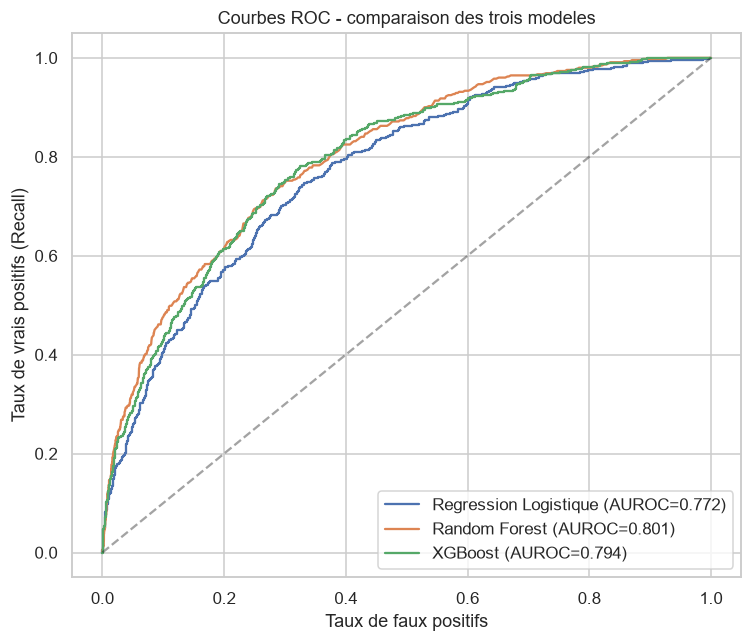
\includegraphics[width=0.62\textwidth]{outputs/courbes_roc.png}
\caption{Courbes \textsc{roc} des trois modèles (échantillon test)}
\label{fig:res-roc}
\end{figure}

\begin{figure}[H]
\centering
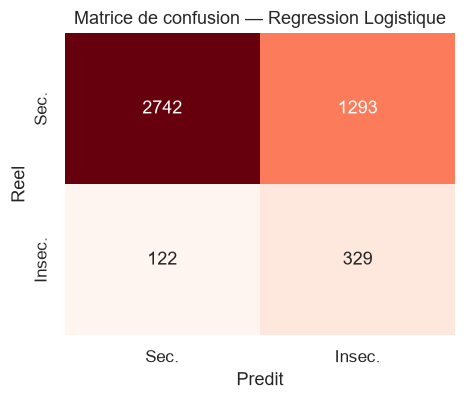
\includegraphics[width=0.45\textwidth]{outputs/matrice_confusion_regression_logistique.png}
\caption{Matrice de confusion de la Régression Logistique (seuil = 0,5)}
\label{fig:res-cm-logit}
\end{figure}

\begin{figure}[H]
\centering
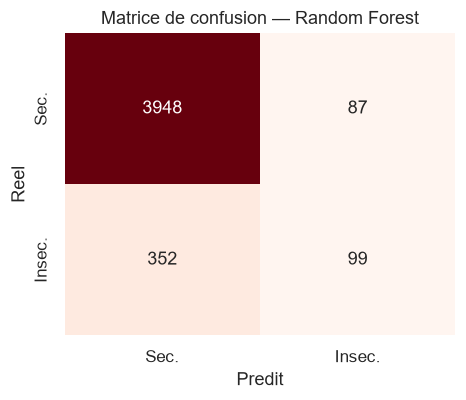
\includegraphics[width=0.45\textwidth]{outputs/matrice_confusion_random_forest.png}
\caption{Matrice de confusion du Random Forest (seuil = 0,5)}
\label{fig:res-cm-rf}
\end{figure}

\begin{figure}[H]
\centering
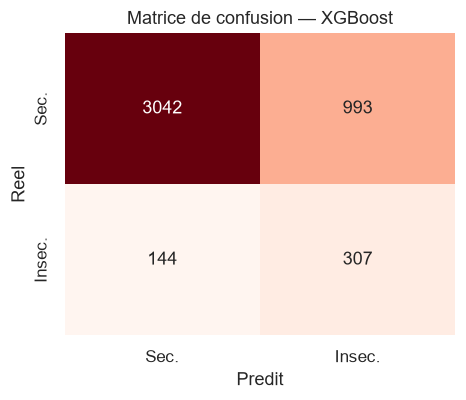
\includegraphics[width=0.45\textwidth]{outputs/matrice_confusion_xgboost.png}
\caption{Matrice de confusion du XGBoost (seuil = 0,5)}
\label{fig:res-cm-xgb}
\end{figure}

\subsubsection{Qualité d'ajustement globale : pseudo-$R^2$ des trois modèles}
\label{sssec:res-pseudor2-comp}

Les trois pseudo-$R^2$ introduits pour le Logit
(Section~\ref{sssec:res-pseudor2}) sont étendus aux deux modèles d'apprentissage
pour comparer la qualité d'ajustement globale des trois approches
(Table~\ref{tab:res-pseudor2}). Une précaution s'impose toutefois : le
\emph{class weighting} \textbf{décalibre volontairement} les probabilités
prédites (il optimise la discrimination, non la vraisemblance), de sorte qu'un
calcul direct sur les probabilités brutes des modèles d'ensemble produirait des
pseudo-$R^2$ négatifs, dénués de sens. Les valeurs inter-modèles sont donc
calculées sur des \textbf{probabilités recalibrées} (régression isotonique
ajustée sur une moitié de l'échantillon test, pseudo-$R^2$ évalué sur l'autre
moitié, sous-ensembles disjoints) ; la valeur classique \emph{in-sample} du
Logit (éq.~14) est rappelée en dernière ligne à titre de référence.

\begin{table}[H]
\centering
\caption{Pseudo-$R^2$ de qualité d'ajustement globale des trois modèles
(probabilités recalibrées sur l'échantillon test, sauf dernière ligne)}
\label{tab:res-pseudor2}
\begin{tabular}{lrrr}
\toprule
\textbf{Modèle} & \textbf{McFadden} & \textbf{Cox-Snell} & \textbf{Nagelkerke} \\
\midrule
Régression Logistique (test recalibré) & 0,147 & 0,091 & 0,191 \\
Random Forest (test recalibré)         & 0,181 & 0,111 & 0,232 \\
XGBoost (test recalibré)               & 0,174 & 0,107 & 0,224 \\
\midrule
Régression Logistique (\emph{in-sample}, éq.~14) & 0,171 & 0,103 & 0,219 \\
\bottomrule
\end{tabular}
\end{table}

Sur des probabilités remises sur un pied de comparabilité, les trois modèles
présentent une qualité d'ajustement globale du même ordre, le
\textbf{Random Forest} (McFadden~=~0,181) et le \textbf{XGBoost}
(0,174) devançant légèrement la régression logistique (0,147). L'ensemble des
pseudo-$R^2$ de McFadden se situe au voisinage du seuil de 0,2 usuellement
associé à un très bon ajustement pour cet indicateur, ce qui conforte, sous un
angle complémentaire à l'\textsc{auroc}, la pertinence des trois modèles et le
léger avantage des méthodes d'ensemble.

\subsubsection{Gestion du déséquilibre : \emph{class weighting} contre \textsc{smote}}

La comparaison prévue à la Section~4.5.2 conforte le choix du
\emph{class weighting} : à hyperparamètres identiques, le XGBoost entraîné sur
données suréchantillonnées par \textsc{smote} obtient une \textsc{auroc}
légèrement inférieure (0,783 contre 0,794) et surtout un \emph{recall}
effondré au seuil de 0,5 (0,118 contre 0,681), rédhibitoire au regard de
l'objectif de détection des ménages vulnérables. Le \emph{class weighting}
présente en outre l'avantage décisif de préserver l'intégration des poids
d'enquête, impossibles à attacher aux observations synthétiques de
\textsc{smote}.

\subsubsection{Analyse de sensibilité à la définition de la variable dépendante}

La hiérarchie des modèles est robuste à la définition de $Y$
(Section~4.2.4) : pour la définition de référence ($\{3,4\}$, prévalence
10,05\,\%) comme pour la définition élargie ($\{2,3,4\}$, 53,20\,\%),
XGBoost domine le Logit (0,794 contre 0,769 et 0,771 contre 0,749
respectivement). Seule la définition stricte ($\{4\}$, 0,83\,\% soit 124~cas)
inverse ponctuellement la hiérarchie (0,814 contre 0,831), inversion à
interpréter avec prudence compte tenu de l'instabilité d'une estimation fondée
sur si peu de cas positifs.

\subsubsection{Calibration des probabilités prédites}

Bruts, les trois modèles sont mal calibrés au sens du test de Hosmer-Lemeshow
($p < 0{,}001$ pour chacun), phénomène attendu : le \emph{class weighting}
optimise la discrimination au détriment de la justesse des probabilités. La
recalibration isotonique du modèle retenu (XGBoost), réalisée sur une moitié de
l'échantillon test et évaluée sur l'autre moitié, corrige ce défaut : le score
de Brier passe de 0,159 à \textbf{0,077} et le test de Hosmer-Lemeshow devient
non significatif ($p = 0{,}479$), indiquant une calibration adéquate
(Figure~\ref{fig:res-calibration}). Le modèle final — XGBoost recalibré — est
donc apte à produire des probabilités interprétables comme des risques réels,
condition posée par l'hypothèse $H_4$ pour le déploiement opérationnel.

\begin{figure}[H]
\centering
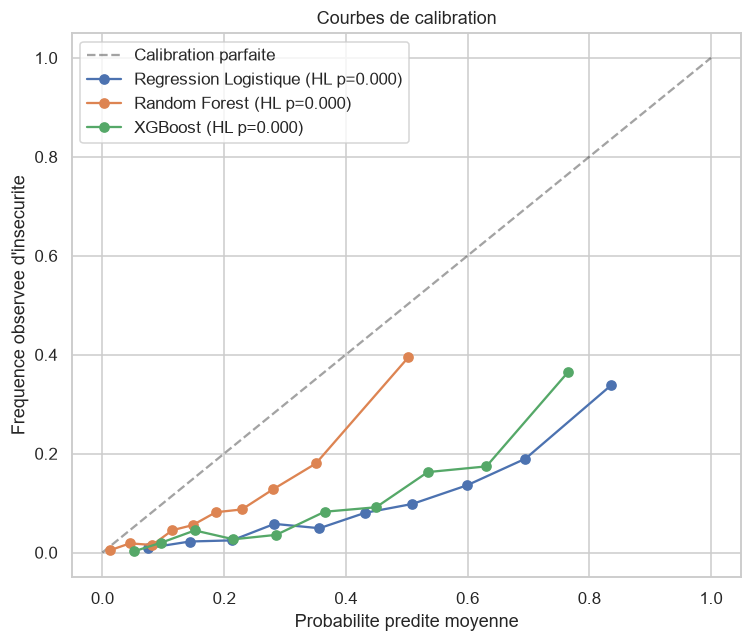
\includegraphics[width=0.62\textwidth]{outputs/calibration.png}
\caption{Courbes de calibration des trois modèles avant recalibration}
\label{fig:res-calibration}
\end{figure}

% ---------------------------------------------------------------------
\subsection{Interprétabilité du modèle retenu : valeurs \textsc{shap}}
\label{ssec:res-shap}

Conformément à la Section~4.7, les valeurs \textsc{shap} ont été calculées pour
les trois modèles (Tree\textsc{shap} pour Random Forest et XGBoost,
Linear\textsc{shap} pour le Logit), sur un échantillon de 1\,200 observations
de l'échantillon test.

\textbf{Importance globale.} Les classements d'importance
(Figure~\ref{fig:res-shap-imp}) convergent avec les déterminants identifiés en
OS1 : les dépenses alimentaires (log), l'accès à l'électricité et le revenu
(log) dominent, suivis de l'indice de qualité du logement et des variables
géographiques (département de l'Atacora). La convergence entre les trois
modèles — pourtant de familles algorithmiques différentes — renforce la
robustesse de ces conclusions.

\textbf{Direction des effets.} Le \emph{summary plot}
(Figure~\ref{fig:res-shap-summary}) confirme le sens des associations : des
dépenses alimentaires faibles, l'absence d'électricité, un revenu faible et un
logement précaire poussent la prédiction vers l'insécurité (valeurs
\textsc{shap} positives), tandis que les niveaux élevés de ces mêmes variables
sont protecteurs.

\textbf{Non-linéarités.} Les \emph{dependence plots} des trois variables les
plus importantes (Figures~\ref{fig:res-shap-dep1}
et~\ref{fig:res-shap-dep2}) révèlent notamment un effet de seuil des dépenses
alimentaires — la contribution au risque devient fortement positive sous un
plancher de dépenses — cohérent avec la non-linéarité détectée par le test de
Box-Tidwell (Section~\ref{ssec:res-bivarie}).

\textbf{Décomposition individuelle.} Les \emph{waterfall plots} de trois
ménages représentatifs illustrent l'usage opérationnel du modèle : pour le
ménage le plus à risque de l'échantillon (probabilité prédite de 0,91 ;
Figure~\ref{fig:res-shap-waterfall}), l'absence de dépenses alimentaires
déclarées (contribution $+0{,}90$ sur l'échelle logit), la résidence dans
l'Atacora ($+0{,}56$), un revenu très faible ($+0{,}16$), l'absence
d'électricité ($+0{,}16$) et l'assistance alimentaire reçue ($+0{,}15$)
constituent l'essentiel du diagnostic. Le
\emph{force plot} interactif du ménage médian, exporté en \textsc{html},
préfigure l'intégration de ces explications individuelles dans l'outil web
(OS4).

\begin{figure}[H]
\centering
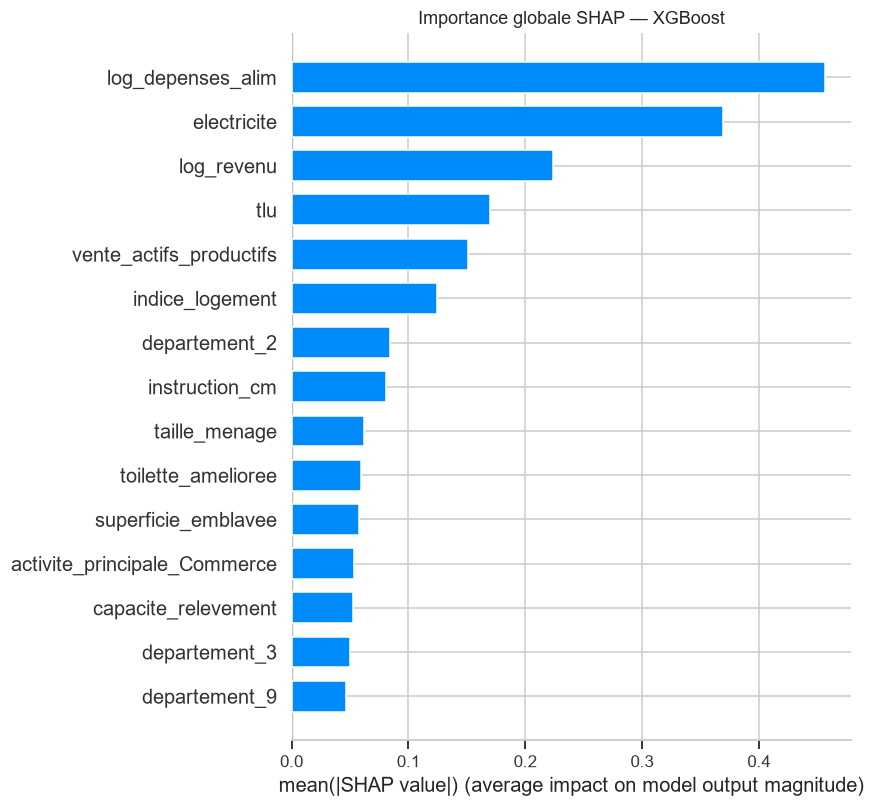
\includegraphics[width=0.72\textwidth]{outputs/shap_importance_xgboost.png}
\caption{Importance globale \textsc{shap} des prédicteurs — XGBoost}
\label{fig:res-shap-imp}
\end{figure}

\begin{figure}[H]
\centering
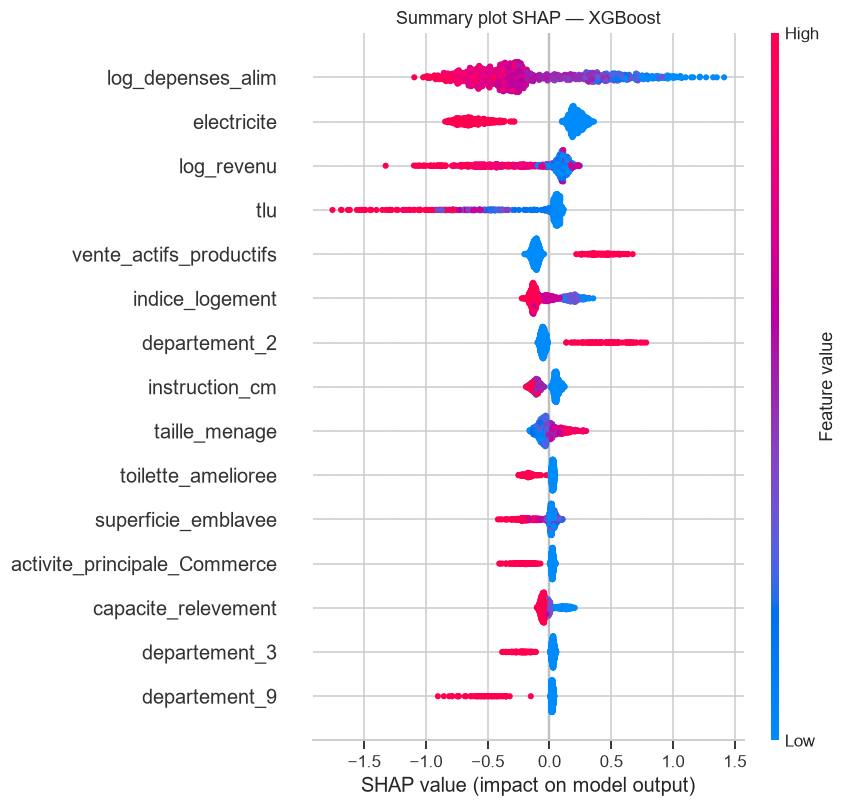
\includegraphics[width=0.72\textwidth]{outputs/shap_summary.png}
\caption{\emph{Summary plot} \textsc{shap} — importance et direction des effets (XGBoost)}
\label{fig:res-shap-summary}
\end{figure}

\begin{figure}[H]
\centering
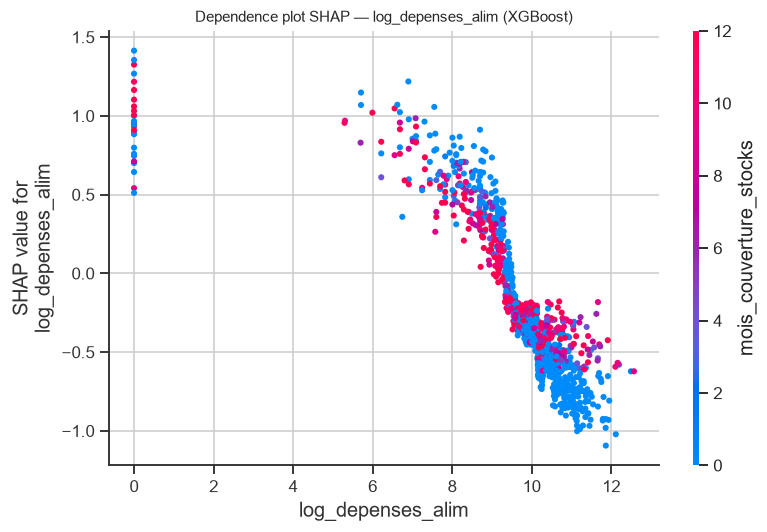
\includegraphics[width=0.6\textwidth]{outputs/shap_dependence_log_depenses_alim.png}
\caption{\emph{Dependence plot} \textsc{shap} des dépenses alimentaires (log)}
\label{fig:res-shap-dep1}
\end{figure}

\begin{figure}[H]
\centering
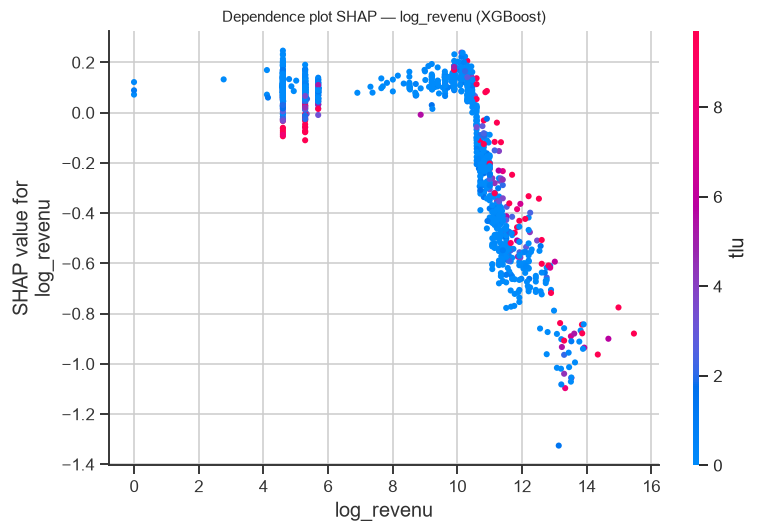
\includegraphics[width=0.6\textwidth]{outputs/shap_dependence_log_revenu.png}
\caption{\emph{Dependence plot} \textsc{shap} du revenu mensuel (log)}
\label{fig:res-shap-dep2}
\end{figure}

\begin{figure}[H]
\centering
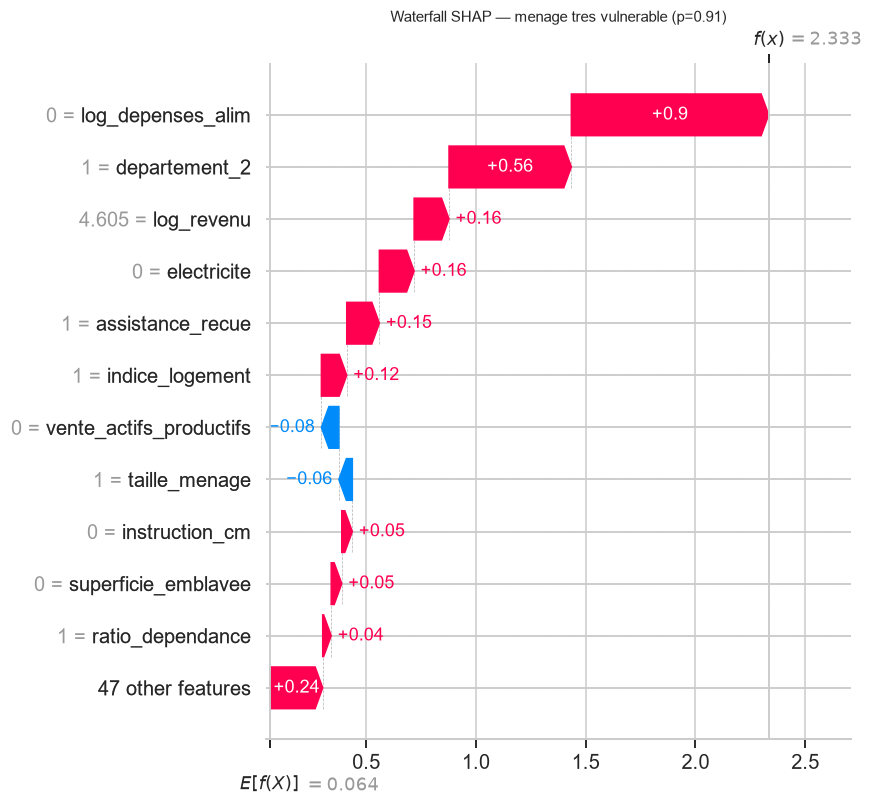
\includegraphics[width=0.72\textwidth]{outputs/shap_waterfall_menage_tres_vulnerable.png}
\caption{\emph{Waterfall plot} \textsc{shap} du ménage le plus vulnérable de l'échantillon
($\hat p = 0{,}91$)}
\label{fig:res-shap-waterfall}
\end{figure}

% ---------------------------------------------------------------------
\subsection{Cartographie communale du risque prédit (OS3)}
\label{ssec:res-os3}

Les probabilités individuelles prédites par le modèle final (XGBoost recalibré)
ont été agrégées par commune avec pondération par les poids d'enquête, puis
jointes au fond de carte des 77~communes (geoBoundaries \textsc{adm}2), avec un
appariement exhaustif (77/77).

\textbf{Autocorrélation spatiale.} L'indice de Moran calculé sur les risques
communaux moyens (matrice de contiguïté de type Queen, standardisée en ligne)
s'établit à $I = 0{,}570$ ($p = 0{,}001$, test par permutations), révélant une
autocorrélation spatiale positive forte et significative : les communes à
risque élevé sont géographiquement groupées. \textbf{L'hypothèse $H_3$ est
confirmée.}

\textbf{Poches de vulnérabilité.} La discrétisation de Jenks en quatre classes
(seuils : 0,08, 0,14 et 0,23) fait apparaître une poche principale de risque
très élevé dans le nord-ouest du pays (département de l'Atacora), et une poche
secondaire dans le centre-sud (Couffo et ouest du Zou)
(Figure~\ref{fig:res-carte}). Les dix communes au risque prédit le plus élevé
sont listées à la Table~\ref{tab:res-communes} : les cinq premières
appartiennent à l'Atacora, Boukoumbé et Toucountouna (39,3\,\% chacune) se
détachant nettement.

\begin{table}[H]
\centering
\caption{Les dix communes au risque prédit d'insécurité alimentaire le plus élevé}
\label{tab:res-communes}
\begin{tabular}{llr}
\toprule
\textbf{Commune} & \textbf{Département} & \textbf{Risque prédit moyen (\%)} \\
\midrule
Boukoumbé    & Atacora & 39,3 \\
Toucountouna & Atacora & 39,3 \\
Tanguiéta    & Atacora & 23,1 \\
Cobly        & Atacora & 22,5 \\
Matéri       & Atacora & 21,5 \\
Agbangnizoun & Zou     & 19,2 \\
Lalo         & Couffo  & 18,9 \\
Natitingou   & Atacora & 18,8 \\
Toviklin     & Couffo  & 17,8 \\
Djakotomey   & Couffo  & 17,4 \\
\bottomrule
\end{tabular}
\end{table}

\begin{figure}[H]
\centering
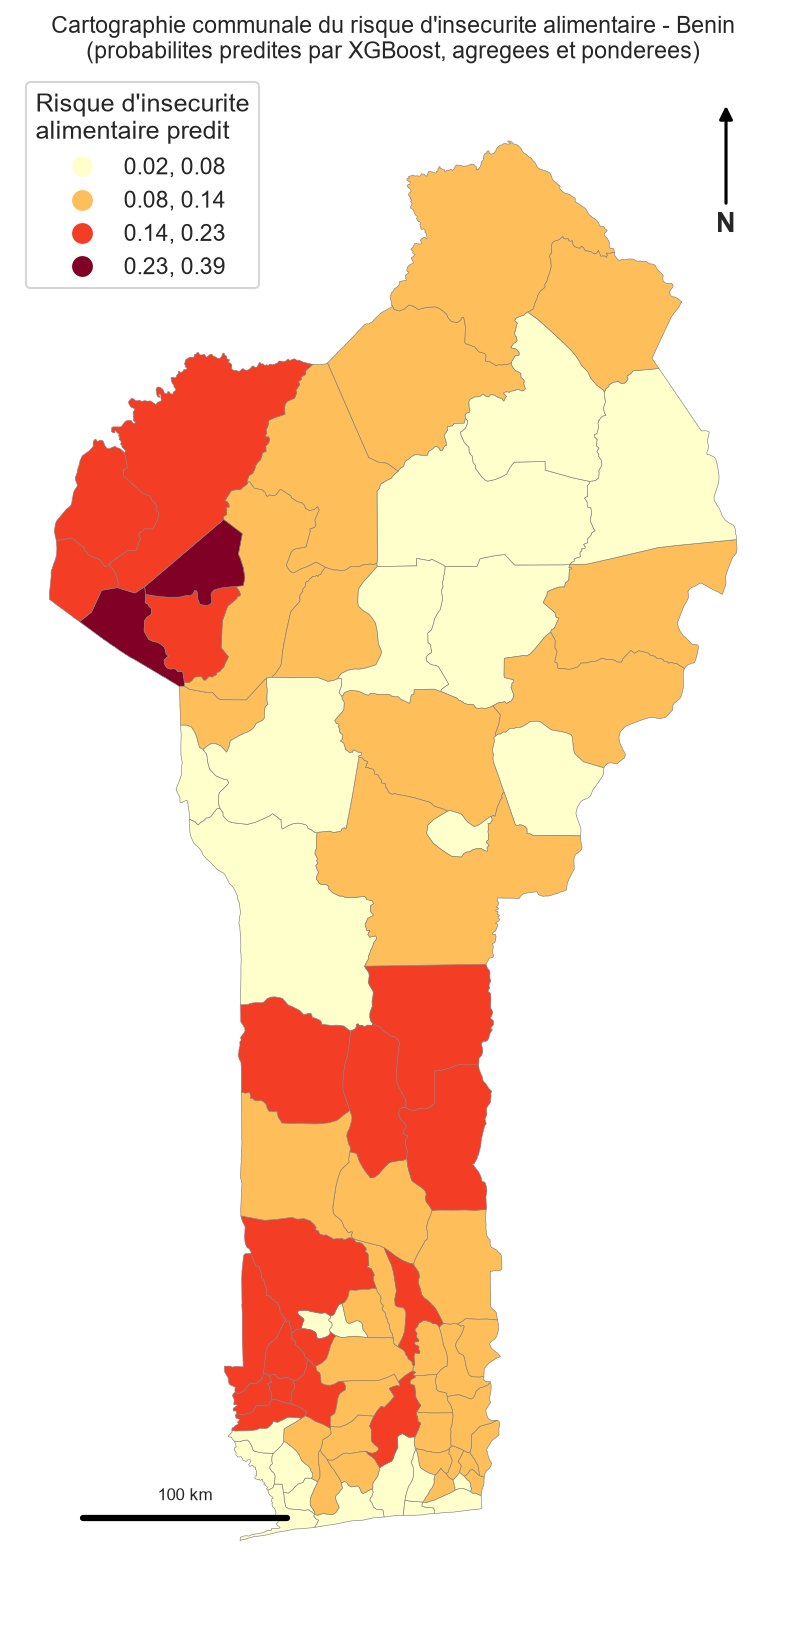
\includegraphics[width=0.8\textwidth]{outputs/carte_risque_communal.png}
\caption{Cartographie communale du risque prédit d'insécurité alimentaire au Bénin
(probabilités du modèle XGBoost, agrégées et pondérées ; discrétisation de Jenks, 4 classes)}
\label{fig:res-carte}
\end{figure}

Ce résultat cartographique converge avec la prévalence départementale observée
(Section~\ref{ssec:res-univarie}) tout en la raffinant à l'échelle communale :
au sein même de l'Atacora, le risque varie du simple au double entre communes,
information directement mobilisable pour le ciblage géographique des
interventions.

% ---------------------------------------------------------------------
\subsection{Produits opérationnels pour l'outil d'aide à la décision (OS4)}
\label{ssec:res-os4}

Le pipeline a produit les artefacts nécessaires au développement de l'outil
d'aide à la décision prévu par l'OS4 :

\begin{itemize}
  \item le \textbf{modèle final sérialisable} (XGBoost recalibré par régression
        isotonique), dont la calibration validée (Brier~=~0,077 ;
        Hosmer-Lemeshow $p = 0{,}479$) autorise des prédictions probabilistes
        fiables sur des ménages hors échantillon au profil similaire à celui de
        l'enquête — condition de l'hypothèse $H_4$ ;
  \item la \textbf{carte interactive} (\texttt{carte\_interactive.html},
        bibliothèque \texttt{folium}) offrant zoom et infobulles communales
        pour la consultation dynamique du risque ;
  \item le \textbf{force plot \textsc{shap} interactif}
        (\texttt{shap\_force\_menage\_median.html}) démontrant la faisabilité
        d'explications individuelles par ménage dans l'application ;
  \item l'\textbf{environnement logiciel figé}
        (\texttt{requirements\_versions.txt}, Section~4.10.1) garantissant la
        reproductibilité du déploiement.
\end{itemize}

Le développement de l'interface applicative elle-même relève des perspectives
et sera discuté au chapitre suivant.

% ---------------------------------------------------------------------
\subsection{Synthèse des résultats au regard des hypothèses de recherche}
\label{ssec:res-hypotheses}

La Table~\ref{tab:res-hypotheses} confronte les résultats obtenus aux quatre
hypothèses formulées au chapitre~2.

\begin{table}[H]
\centering
\caption{Confrontation des résultats aux hypothèses de recherche}
\label{tab:res-hypotheses}
\begin{tabular}{p{0.16\textwidth}p{0.5\textwidth}p{0.24\textwidth}}
\toprule
\textbf{Hypothèse} & \textbf{Résultat empirique} & \textbf{Verdict} \\
\midrule
$H_1$ (OS1) & Éducation (OR = 0,831 ; $p$ = 0,007) et diversification des
revenus (OR = 0,823 ; $p$ = 0,036) significatives ; eau améliorée et résidence
rurale significatives au stade bivarié mais non retenues par le modèle
multivarié (effets absorbés par l'habitat et le département). &
Partiellement validée \\
\addlinespace
$H_2$ (OS2) & AUROC : RF 0,801 $\approx$ XGBoost 0,794 $>$ Logit 0,773 ;
DeLong ML vs Logit significatif ($p \leq 5\times10^{-4}$) ; hiérarchie robuste
aux définitions de $Y$ (hors définition stricte, 124 cas). & Validée \\
\addlinespace
$H_3$ (OS3) & Indice de Moran $I$ = 0,570 ($p$ = 0,001) ; poches concentrées
dans l'Atacora (nord-ouest), secondairement Couffo--Zou. & Validée \\
\addlinespace
$H_4$ (OS4) & Après recalibration isotonique : Brier = 0,077 ;
Hosmer-Lemeshow $p$ = 0,479 ; artefacts opérationnels produits (carte et
explications interactives). & Validée \\
\bottomrule
\end{tabular}
\end{table}

En résumé, l'étude identifie un noyau robuste de déterminants — conditions
économiques du ménage (dépenses, revenu, diversification), capital humain
(instruction, scolarisation), habitat (électricité, qualité du logement) et
ancrage territorial (Atacora) — convergents entre l'approche économétrique
(odds ratios) et l'approche prédictive (valeurs \textsc{shap}) ; elle établit
la supériorité discriminante des algorithmes d'ensemble sur la régression
logistique, sélectionne et calibre un modèle XGBoost opérationnel, et localise
les poches communales de vulnérabilité qui fondent le ciblage géographique des
interventions. Ces résultats sont discutés et mis en perspective au chapitre
suivant.

% ===================== FIN DU CHAPITRE 5 =============================
